%% Copyright 2007-2018 Elsevier Ltd
%% 
%% This file is part of the 'Elsarticle Bundle'.

%% ---------------------------------------------
%% 
%% It may be distributed under the conditions of the LaTeX Project Public
%% License, either version 1.2 of this license or (at your option) any
%% later version.  The latest version of this license is in
%%    http://www.latex-project.org/lppl.txt
%% and version 1.2 or later is part of all distributions of LaTeX
%% version 1999/12/01 or later.
%% 
%% The list of all files belonging to the 'Elsarticle Bundle' is
%% given in the file `manifest.txt'.
%% 
%% Template article for Elsevier's document class `elsarticle'
%% with harvard style bibliographic references

%\documentclass[preprint,12pt,authoryear]{elsarticle}

%\documentclass[twocolumn,12pt,authoryear]{elsarticle}
%% Use the option review to obtain double line spacing
%\documentclass[authoryear,preprint,review,12pt]{elsarticle}

%% Use the options 1p,twocolumn; 3p; 3p,twocolumn; 5p; or 5p,twocolumn
%% for a journal layout:
%%\documentclass[final,1p,times,authoryear]{elsarticle}
%%\documentclass[final,1p,times,twocolumn,authoryear]{elsarticle}
%%\documentclass[final,3p,times,authoryear]{elsarticle}
\documentclass[final,3p,times,twocolumn,authoryear]{elsarticle}
%%\documentclass[final,5p,times,authoryear]{elsarticle}
%%\documentclass[final,5p,times,twocolumn,authoryear]{elsarticle}

%% For including figures, graphicx.sty has been loaded in
%% elsarticle.cls. If you prefer to use the old commands use
%%\usepackage{epsfig}
%% The amssymb package provides various useful mathematical symbols
%\usepackage{amssymb}
%% The amsthm package provides extended theorem environments
%% \usepackage{amsthm}
\usepackage{graphicx}% Include figure files
%\usepackage{pdflscape}
\usepackage{rotating}
\usepackage{array}
\usepackage{dcolumn,multirow}

% Align table columns on decimal point
%% The lineno packages adds line numbers. Start line numbering with \begin{linenumbers} and end with \end{linenumbers}
%% Or switch it on
\usepackage{lineno}
\linenumbers
\journal{Nuclear Instruments and Methods A}
\begin{document}
\begin{frontmatter}
%% Title, authors and addresses
%% use the tnoteref command within \title for footnotes;
%% use the tnotetext command for theassociated footnote;
%% use the fnref command within \author or \addoratorytnote;
%% use the corref command within \author for corresponding author footnotes;
%% use the cortext command for theassociated footnote;
%% use the ead command for the email address,
%% and the form \ead[url] for the home page:
%% \title{Title\tnoteref{label1}}
%% \tnotetext[label1]{}
%% \author{Name\corref{cor1}\fnref{label2}}
%% \ead{email address}
%% \ead[url]{home page}
%% \fntext[label2]{}
%% \cortext[cor1]{}
%% \address{Address\fnref{label3}}
%% \fntext[label3]{}
\title{The CLAS12 Spectrometer at Jefferson Laboratory}
%% use optional labels to link authors explicitly to addresses:
%% \author[label1,label2]{}
%% \address[label1]{}
%% \address[label2]{}
\author{V. D. Burkert, L. Elouadrhiri, D. Anderson, S. Aune, H. Avakian, N. Baltzell, M. Battaglieri,  V. Baturin, S. Boiarinov,
  P. Bonneau, K. Bruhwel, D. Carman, A. Celentano, M. Contalbrigo, S. Christo, M. Defurne, G. Dodge, R. De Vita, K. Giovanetti,
  F.X. Girod, L. Guo, R. Gothe, Y. Gotra, K. Hafidi, D. Heddle, K. Hicks, D. Insley, K. Joo,  D. Kashy, A. Kim, W. Kim, V. Kubarovski,
  S. Kuhn, M. Mcmullen, I. Mandjavidze, N. Markov, C. Mealer, M. Mestayer, Z.E. Meziani, R. Miller, M. Mirazita, S. Niccolai,
  O. Pastor, E. Pasyuk, O. Pogorelko, B. Raue, P. Rossi, F. Sabatie, Y. Sharabian, S. Stepanyan, M. Ungaro, A. Vlassov, L. Weinstein,
  C. Wiggins, A. Yegneswaran, G. Young, V. Ziegler, more coming ............. }
\address{12000 Jefferson Avenue, Newport News, Virginia, 23606}
%\author{ K. Hafidi,  .......} 
\address{ Argonne National Laboratory, Argonne, Illinois, 60439, USA}
%\author{D. Heddle, ........}
\address{Christopher Newport University, Newport News, Virginia 23605, USA} 
%\author{K. Joo, A. Kim, N. Markov, ........} 
\address{University of Connecticut, Storrs, Connecticut 06269, USA} 
%\author{A. Biselli,..}
%\address{Fairfield University, Fairfield, Connecticut 06824, USA}
%\author{L. Guo, B. Raue, ...}
\address{Florida International University, Miami, Florida, 33199, USA} 
%\author{S. Aune, M. Defurne, I. Mandjavidze, F. Sabatie, ....... }
\address{IRFU, CEA, Universit{\'e} Paris-Saclay, F-91191 Gif-sur-Yvette, France}
%\author{M. Battaglieri, A. Celentano, R. De Vita, .....}
\address{INFN, Sezione di Genova, 16146 Genova, Italy}
%\author{P. Chatagnon, S. Niccolai, ......}
\address{Institut de Physique Nucl{\'e}aire, IN2P3-CNRS, Universit{\'e} Paris-Sud,  Universit{\'e} Paris-Saclay, F-91406 Orsay,
  France}
%\author{O. Pogorelko, A. Vlassov, ....} 
\address{Institute of Theoretical and Experimental Physics, Moscow, Russia}
%\author{G. Dodge, S. Kuhn, L. Weinstein,  Victoria xxx, ........}
\address{Old Dominion University, Norfolk, Virginia, 23529, USA} 
%\author{R. Gothe, ...................}
\address{University of South Carolina, Columbia, South Carolina 29208}
%\author{ K. Hicks, ....} 
\address{ Ohio University, Athens, Ohio, 45701}
%\author{P. Cole, T. Forrest, K. Hicks, .........}
\address{Idaho State University, Pocatello, Idaho, 83209, USA}
%\author{M. Contalbrigo, .......}
\address{INFN, Sezione di Ferrara, 44100 Ferrara, Italy}  
%\author{M. Mirazita, .......}
\address{INFN, Laboratori Nazionali di Frascati, 00044 Frascati, Italy}
%\author{K. Giovanetti, ......}
\address{James Madison University, Harrisonburg, Virginia 22807, USA}
%\author{W. Kim, .....}
\address{Kyungpook National University, Daegu 41566, Republic of Korea}
%\address{ .......................................... }
%\vspace{-0.5cm}

\begin{abstract}
  The CEBAF Large Acceptance Spectrometer for operation at 12~GeV beam energy (CLAS12) at Jefferson Laboratory is
  used to study electro-induced nuclear and hadronic reactions, and provides efficient detection of charged and neutral
  particles over a large fraction of the full solid angle. CLAS12 has been part of the energy-doubling project of Jefferson
  Lab's Continuous Wave Electron Beam Accelerator Facility, funded by the United States Department of Energy. A
  collaboration of over 40 institutions contributed to the design and construction of detector hardware, developed the 
  software packages for the simulation of complex event patterns, and commissioned the detector systems. CLAS12 is based
  on a dual magnet system with a superconducting Torus magnet covering the forward angle range that provides a largely
  azimuthal field distribution, and a solenoid magnet and detector covering the polar angles from $40^\circ$ to $125^\circ$,
  with full azimuthal coverage. Trajectory reconstruction in the forward direction using drift chamber and in the central
  direction using vertex tracker results in momentum resolutions of  $< 1\%$ and $< 3\%$, respectively.  Cherenkov counters, 
  time-of-flight scintillators, and electromagnetic calorimeters provide good particle identification. Fast triggering and high
  data-acquisition rates allow operation at a luminosity of $10^{35}$~cm$^2$s$^{-1}$. These capabilities are being used in a
  broad program to study the structure and interactions of nucleons, nuclei, and mesons using polarized and unpolarized
  electron beams and targets for beam energies up to 11~GeV. This paper gives a general description of the design,
  construction, and performance of CLAS12.  
\end{abstract}

\end{frontmatter}

\linenumbers
\section{Introduction}
%\label{Intro}

Electron scattering has been proven an effective way of probing the size and internal structure of subatomic particles as
protons, neutrons, and nuclei. Exploiting energetic electron beams led to rapid progress in our understanding of the internal
composition of particles. The extended size of the proton was first mapped out in the mid 1950's~\cite{Mcallister:1956ng} ,
and the internal quark substructure was discovered in the late 1960's~\cite{Breidenbach:1969kd}. Using spin polarized
electrons and spin polarized targets, the internal quark helicity momentum distribution was mapped out in the 1980's and the
following decades, and is still an important research topic today~\cite{Kuhn:2008sy}. These experiments only required
inclusive measurements, where only the beam particle, electrons or muons, that scattered off the target were detected
and kinematically analyzed.  

\begin{figure}[htbp]
\vspace{4.5cm}
\begin{picture}(50,50)
\put(-20,-20)
{\hbox{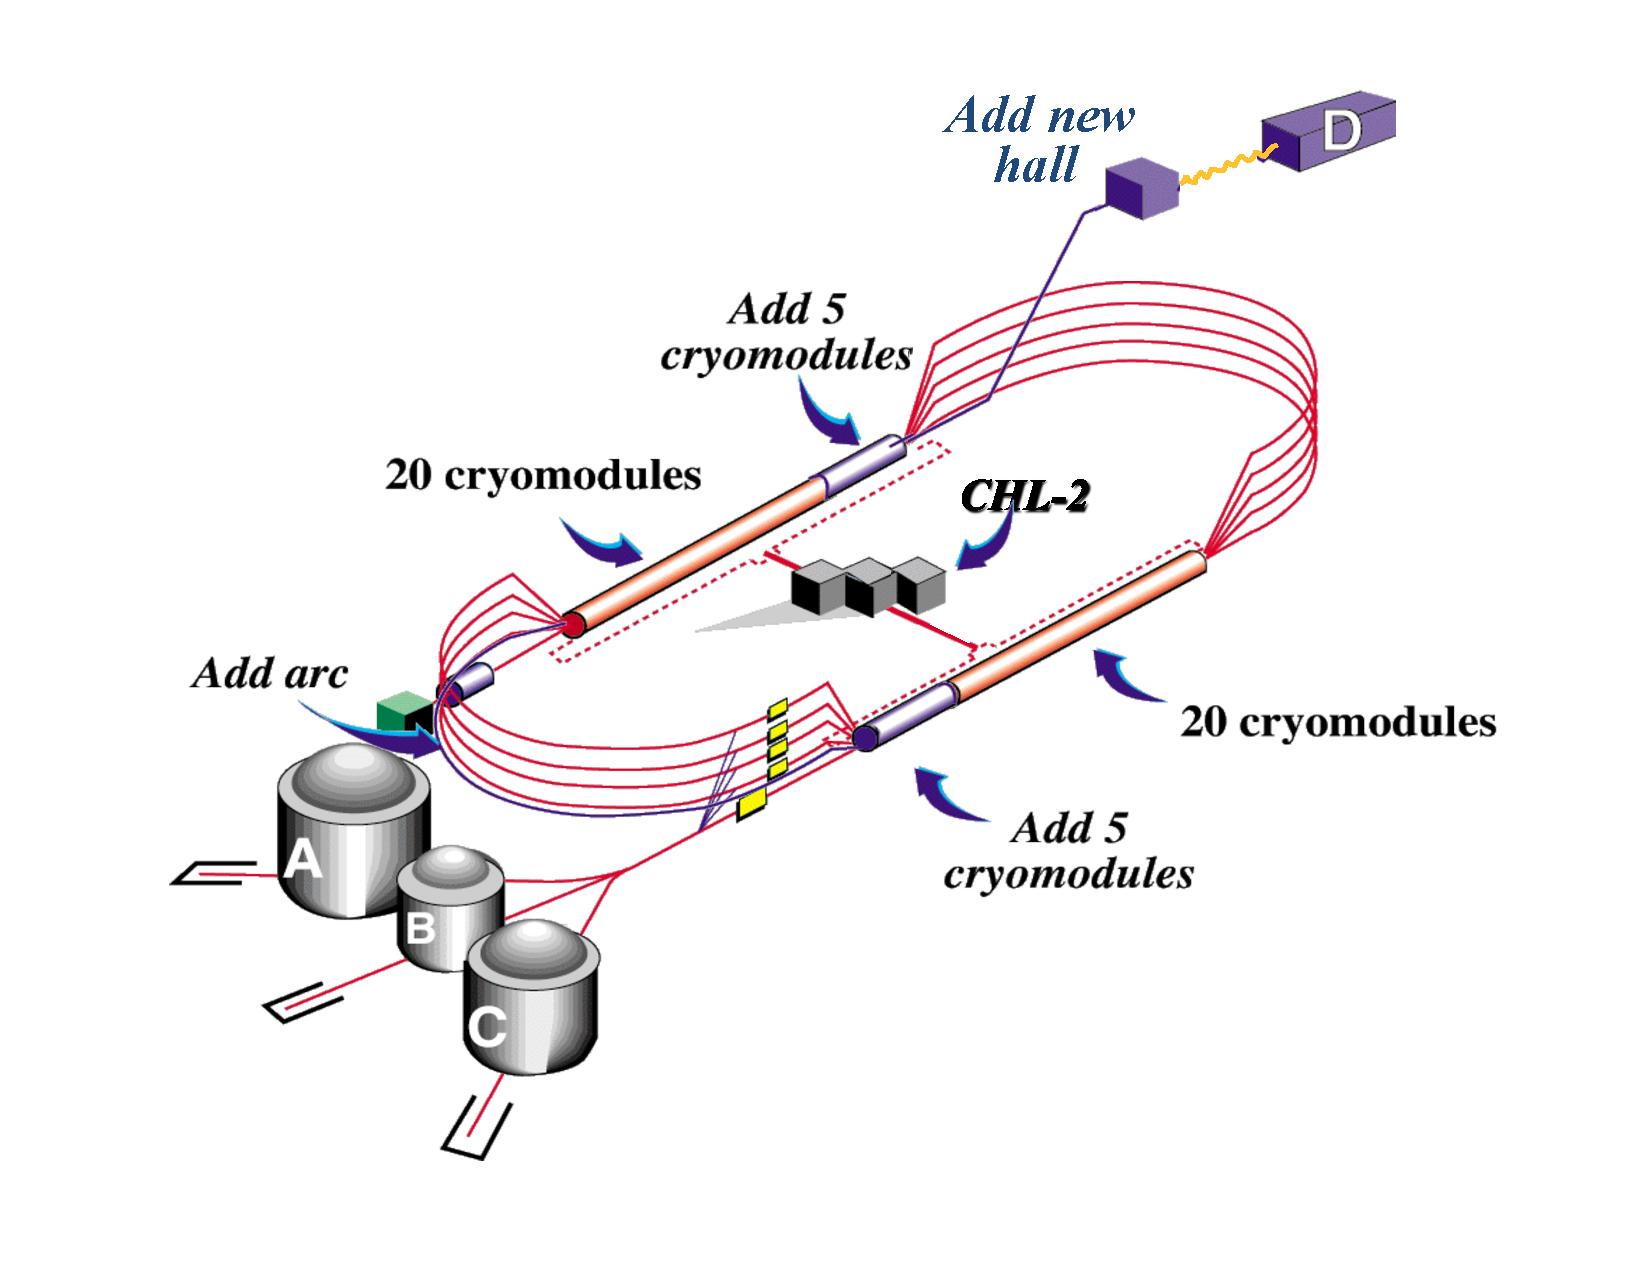
\includegraphics[width=0.43\textwidth,natwidth=610,natheight=642]{cebaf.pdf}}}
\end{picture} 
\caption{The CEBAF continuous electron beam accelerator after the doubling of the beam energy to 12~GeV and adding
  Hall~D as a new experimental end station for photon physics experiments.The accelerator is 1,400~m in circumference. }
\label{cebaf12}
\end{figure}  

In the decades following these discoveries, it was realized that a more detailed understanding of the internal structure of
nucleons requires  the reconstruction of fully exclusive or semi-inclusive processes, and hence the detection and kinematical
reconstruction of additional mesons and baryons in the final state was required.  Other constraints came from the desire of
baryon spectroscopy to measure complete angular distributions, which made it necessary to employ large acceptance devices
to serve that purpose. The Continuous Electron Beam Accelerator Facility (CEBAF)~\cite{Leemann:2001dg}, the CLAS
detector~\cite{Mecking:2003zu}, and other experimental equipment at Jefferson Laboratory (JLab) were designed and
constructed in the 1990's with these goals in mind and were operated successfully for over 15 years. 
 
The further development of Quantum Chromodynamics (QCD) as the theory of the interaction of colored quarks and gluons,
combined with the discovery of the Generalized Parton Distributions (GPDs) provided a novel way that allowed describing the
nucleon structure in 3 dimensions, 2 in coordinate space and 1 in momentum space. The discovery opened up a new avenue of
hadronic research that has become one of the flagship programs in nuclear and hadronic physics. The GPDs must be probed in
exclusive processes, with deeply virtual Compton scattering being the most suitable one, and in a large kinematic space. This is
a rather rare process and measurements require high intensity electron (or muon) beams and large acceptance detectors to
provide sufficient rate to map out the process in the full kinematic phase space using polarized beams, polarized targets, and
sufficiently high beam energy. The complementary process of semi-inclusive deep inelastic scattering (SIDIS) is also of topical
interest,  which also probes the nucleon's internal structure in 3D momentum space. The science program of CLAS12 is very
broad~\cite{Burkert:2018nvj} and encompasses the study of the structure of the proton and neutron both in their ground state,
as well as their many excited states, and in the deeply inelastic kinematics. Other experiments are designed to probe the short
range structure of nuclei through measurement of the transparency of nuclei to mesons and baryons, and how it changes with
the momentum transfer.   

\begin{figure*}[ht]
\vspace{6.0cm}
\begin{picture}(50,50)
\put(30,-5)
{\hbox{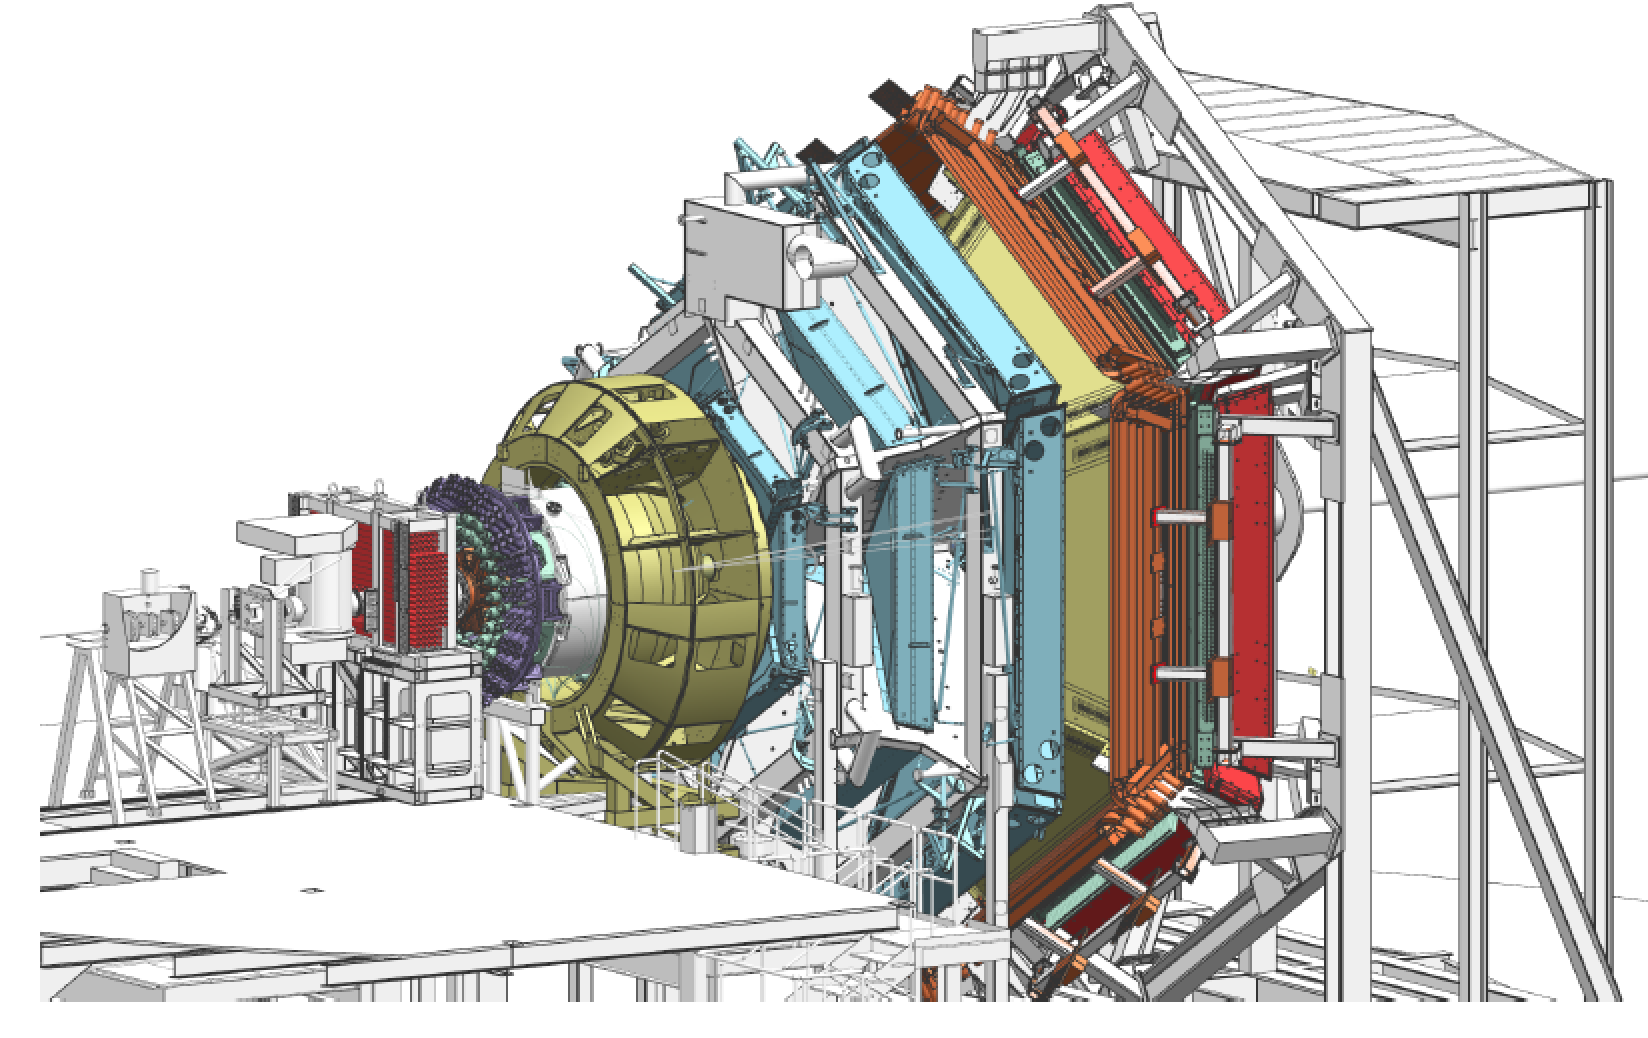
\includegraphics[width=0.45\textwidth,natwidth=610,natheight=642]{CLAS12.png}}}
\end{picture} 
\caption{The electron beam enters from the left and enters the production target located in the center of the solenoid
  magnet shown at the left (upstream) end of CLAS12, where also other detector components are visible. Scattered electrons
  and forward-going particles are detected in the Forward Detector (FD) consisting of a high-threshold Cherenkov counter
  (HTCC) with full coverage in polar angle $5^\circ \le \theta \le 35^\circ$ and $\Delta \phi = 2\pi$ coverage in azimuth. The
  HTCC is followed by the Torus magnet, the drift chamber (DC) tracking system, another set of Cherenkov counters (LTCC,
  RICH), time-of-flight scintillation counters (FTOF), and electromagnetic calorimeters (ECAL). The DCs are supported from
  the Torus magnet. The detectors downstream of the Torus magnet are mounted on a separate Forward Carriage that is
  independently movable to allow access to the detectors for maintenance. The Central Detector (CD) consists of the silicon
  vertex tracker (SVT), which is surrounded by a barrel micromesh tracker (BMT), the Central Time-of-Flight (CTOF) counter,
  and the central neutron detector (CND). The entire CLAS12 detector extends for 20~m along the beamline.} 
\label{clas12}
\end{figure*}

\section{The JLab Facility at 12~GeV}
\label{jlab}

 The CLAS12 detector was designed to study electro-induced nuclear and hadronic reactions by providing efficient detection
 of charged and neutral particles over a large fraction of the full solid angle. A collaboration of over 40 institutions has
 participated in the design, fabrication, assembly, and final commissioning of CLAS12 in Hall~B at the Thomas Jefferson
 National Accelerator Facility. The CLAS12 detector is based on a combination of a six-coil Torus magnet and a high-field
 Solenoid magnet. The combined magnetic field provides a large coverage in both azimuthal and polar angles. Trajectory
 reconstruction using drift chambers at forward angles results in a momentum resolution of ${\sigma_p / p} \approx 0.005$.
 At large polar angles, where particle momenta are typically below 1~GeV, the vertex resolution is
 $\approx 200-300$~$\mu$m ({\bf put correct values in}) with momentum resolutions of $\sigma_p / p \approx 0.03$
 ({\bf put correct values here}).  Cherenkov counters, time-of-flight systems, and calorimeters provide good particle
 identification for electrons, charged pions, kaons, and protons. Fast triggering and high data acquisition rates allow operation
 in luminosities of $10^{35}$~cm$^{-2}$s$^{-1}$ for extended periods of time. These capabilities are being used in a
 broad scientific program to study the structure and interactions of baryons, meson, and nuclei using polarized and unpolarized
 targets. 

\begin{figure*}[htbp]
\vspace{5.7cm}
\begin{picture}(50,50)
\put(55,0)
{\hbox{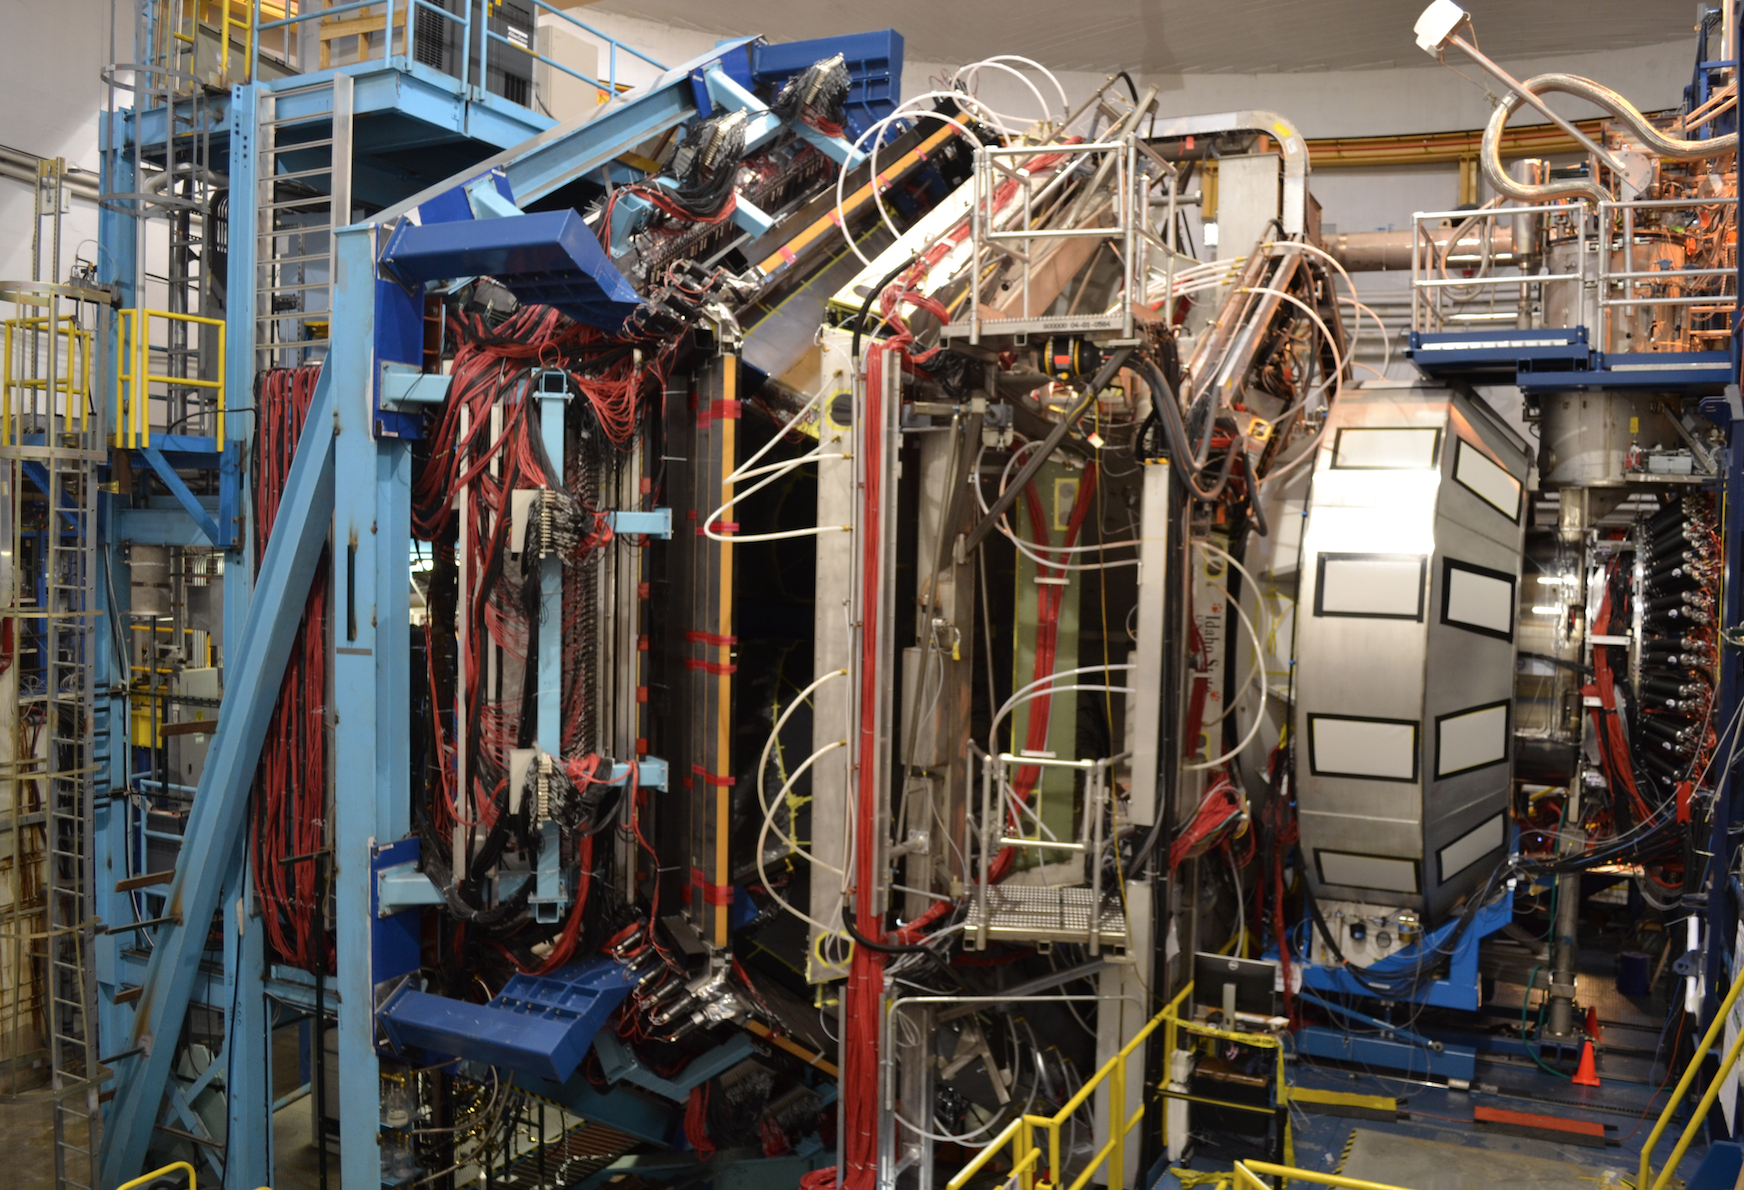
\includegraphics[width=0.35\textwidth,natwidth=610,natheight=642]{CLAS12-photo.png}}}
\end{picture} 
\caption{The CLAS12 detector in the Hall~B beamline. The beam is entering from the right near the upstream end of the
  Solenoid magnet and the cryogenics service tower, followed by the HTCC and the Torus magnet with the forward
  tracking detectors.  LTCC and the calorimeters, PCAL and EC are seen at the down stream end to the left. }
\label{clas12-photo}
\end{figure*}

This paper provides a general description of the design, construction, and performance of CLAS12 and how it expands upon
the capabilities provided by the JLab 12~GeV energy upgrade. The CEBAF accelerator and experimental halls are shown for
the energy upgraded configuration in Fig.~\ref{cebaf12}. CEBAF is designed from two parallel linear accelerators based on
superconducting radio frequency (RF) technology, and arranged in a race-track configuration~\cite{Leemann:2001dg}. Spin
polarized electrons are generated in the gun,  pre-accelerated in the injector, and subsequently injected and accelerated in
the north linac. They are then bent in a $180^\circ$ arc and injected into the south linac. This is repeated four and a half more
times to reach the final energy for Hall~D and up to four times  for the desired delivery energies to Halls~A, B, and C. In the
recirculating arcs, electrons are transported in 5 independent out-of-phase tracks of different energies. For 12~GeV operation,
five accelerating cryomodules with four times higher gradients than were used in the 6~GeV CEBAF machine were added to each
of the two existing linear accelerators to reach a maximum energy of 10.9~GeV for Halls~A, B, and C. One added arc path and
one more pass through the north linac were added to achieve the highest beam energy of 12~GeV for Hall~D. This highest
beam energy is generated exclusively for Hall~D, while the other three halls may receive beams at the same beam energy or
at different beam energies simultaneously, with up to a factor $10^5$ differences in current from 1~nA to 100~$\mu$A.

\begin{figure}[htbp]
\vspace{6.0cm}
\begin{picture}(50,50)
\put(12,0)
{\hbox{\includegraphics[width=0.37\textwidth,natwidth=610,natheight=642]{clas12-fd.png}}}
\end{picture} 
\caption{Forward Detector as seen from the beamline before the installation of the drift chamber tracking system. The six
  structures extending radially from the apex are the cryostats of the individual Torus magnet coils. The steel cross bars in
  the middle of the sectors supported the coils during magnet assembly, and were removed before operation. When energized
  the magnetic field lines loop around the azimuth, falling in strength approximately as the inverse of the radial distance from
  the magnet center.  {\bf FIND PHOTO WITH BETTER LIGHTINGS}}
\label{clas12-fd}
\end{figure}

Major new detectors and other experimental equipment have been installed in Halls~B, C, and D that support a broad science
program of nuclear and hadronic physics. In Hall~D, a large hermetic detector with a solenoid magnet at its core has been in
operation since 2015. It incorporates tracking capabilities and photon detection over nearly the full $4\pi$ solid angle. This
Hall is dedicated to the production of mesons employing a linearly polarized photon beam. The new CLAS12 spectrometer,
displayed in a side view in Fig.~\ref{clas12}, features large solid angle coverage and instantaneous luminosities of up to
$10^{35}$~cm$^{-2}$s$^{-1}$ for electron scattering experiments with multiple particle final states. 

Hall~C includes the new super-high momentum magnetic spectrometer (SHMS) in addition to the existing high momentum
spectrometer (HMS). In Hall~A, a new super big bite spectrometer (SBS) has been added to the existing high resolution 
spectrometer pair HRS$^2$, and other large installation experiments have been proposed. Complementing the new equipment
is the highly spin-polarized electron gun, high power cryogenic targets, and several spin-polarized targets using NH$_3$,
ND$_3$, HD, $^3$He, and $^7$Li as target materials to support a broad range of polarization measurements.   

\begin{figure}[htbp]
\vspace{2.5cm}
\begin{picture}(50,50)
\put(12,0)
{\hbox{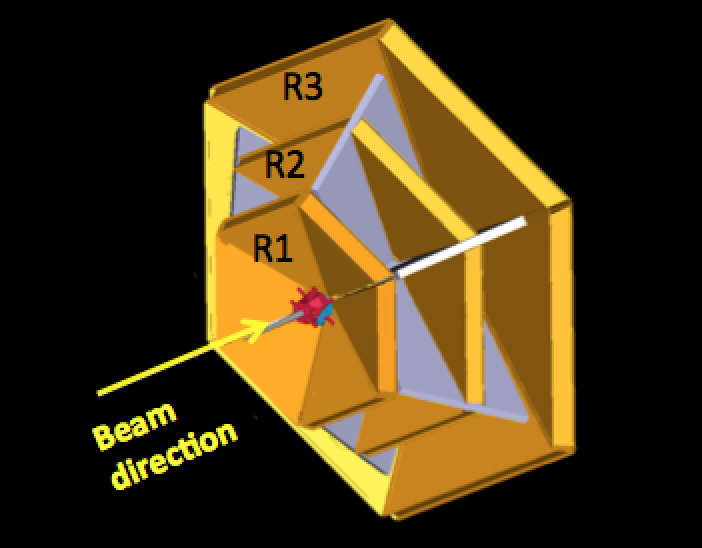
\includegraphics[width=0.50\textwidth,natwidth=610,natheight=642]{CLAS12-DC.png}}}
\end{picture} 
\caption{3D concept of the drift chamber arrangement in CLAS12 tracking  system. R1 chambers are located just in front
  of the Torus magnet coils (gray shade) . R2 chambers are sandwiched between the coils of the magnet, and R3 are located
  just behind the magnet.  {\bf REPLACE WITH ENGINEERING DRAWING.}}
\label{clas12-dc}
\end{figure}

\begin{figure}[htbp]
\vspace{2.5cm}
\begin{picture}(50,50)
\put(12,0)
{\hbox{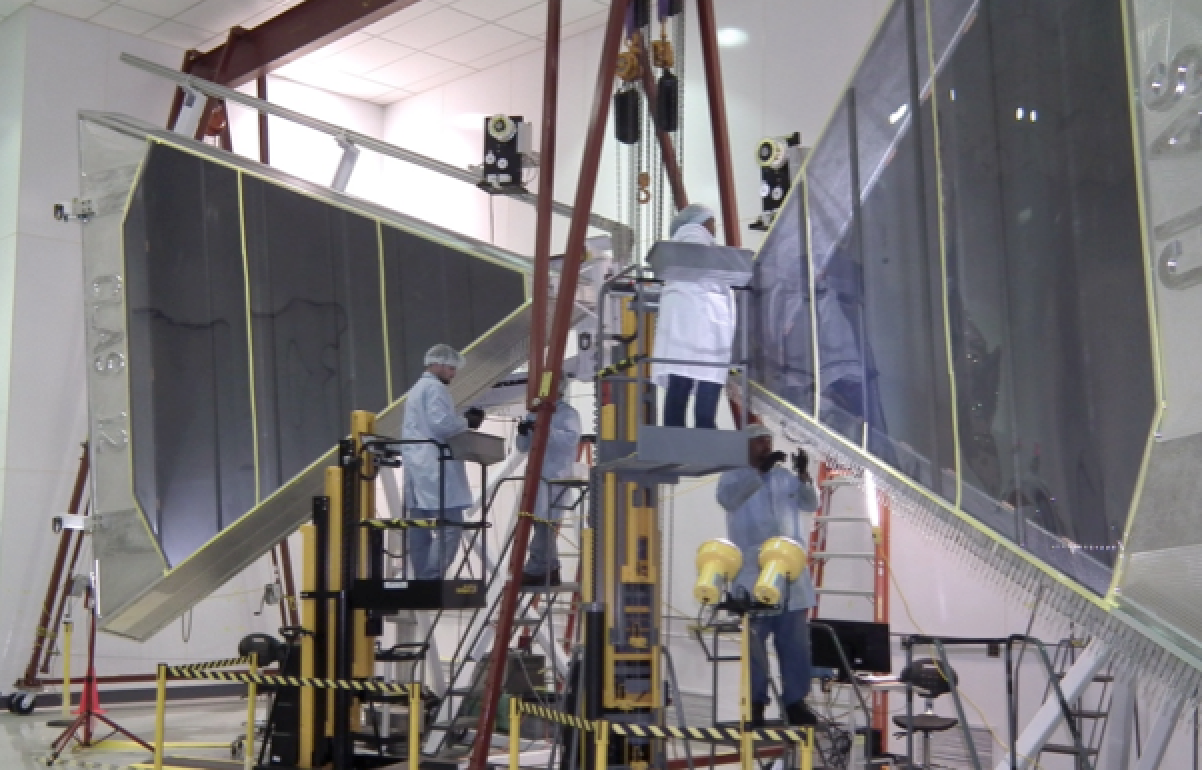
\includegraphics[width=0.30\textwidth,natwidth=610,natheight=642]{DC-R3.png}}}
\end{picture} 
\caption{Wire stringing of two R3 chambers in the Jefferson Lab clean room. {\bf DO WE HAVE HIGHER
  RESOLUTION PHOTO?}}
\label{dc-stringing}
\end{figure}

\section{The CLAS12 Forward Detector (FD)}

The design of CLAS12 is based on a combination of a toroidal magnetic field at polar angles up to $\approx 35^\circ$ and a
5~T solenoidal field at central angles in the approximate polar angle range $35^\circ~\le \theta \le~125^\circ$. The primary
requirement driving this choice is the ability to measure charged particles at high momentum with good resolution at forward
angles, while operating the detector systems at high luminosity. This requires effective shielding of the detector system from
low energy electrons produced in the target material due to M\"oller scattering $e^- + e^- \to e^- + e^-$ of the high-energy
beam electrons on atomic electrons in the target material. The large majority of those electrons are prevented from reaching 
sensitive detectors as they curl up in the strong longitudinal magnetic solenoid field, and are then guided into a shielding pipe 
made from bulk tungsten material where they dump their energy. 

\begin{figure}[htbp]
\vspace{5.0cm}
\begin{picture}(50,50)
\put (-37,190)
{\hbox{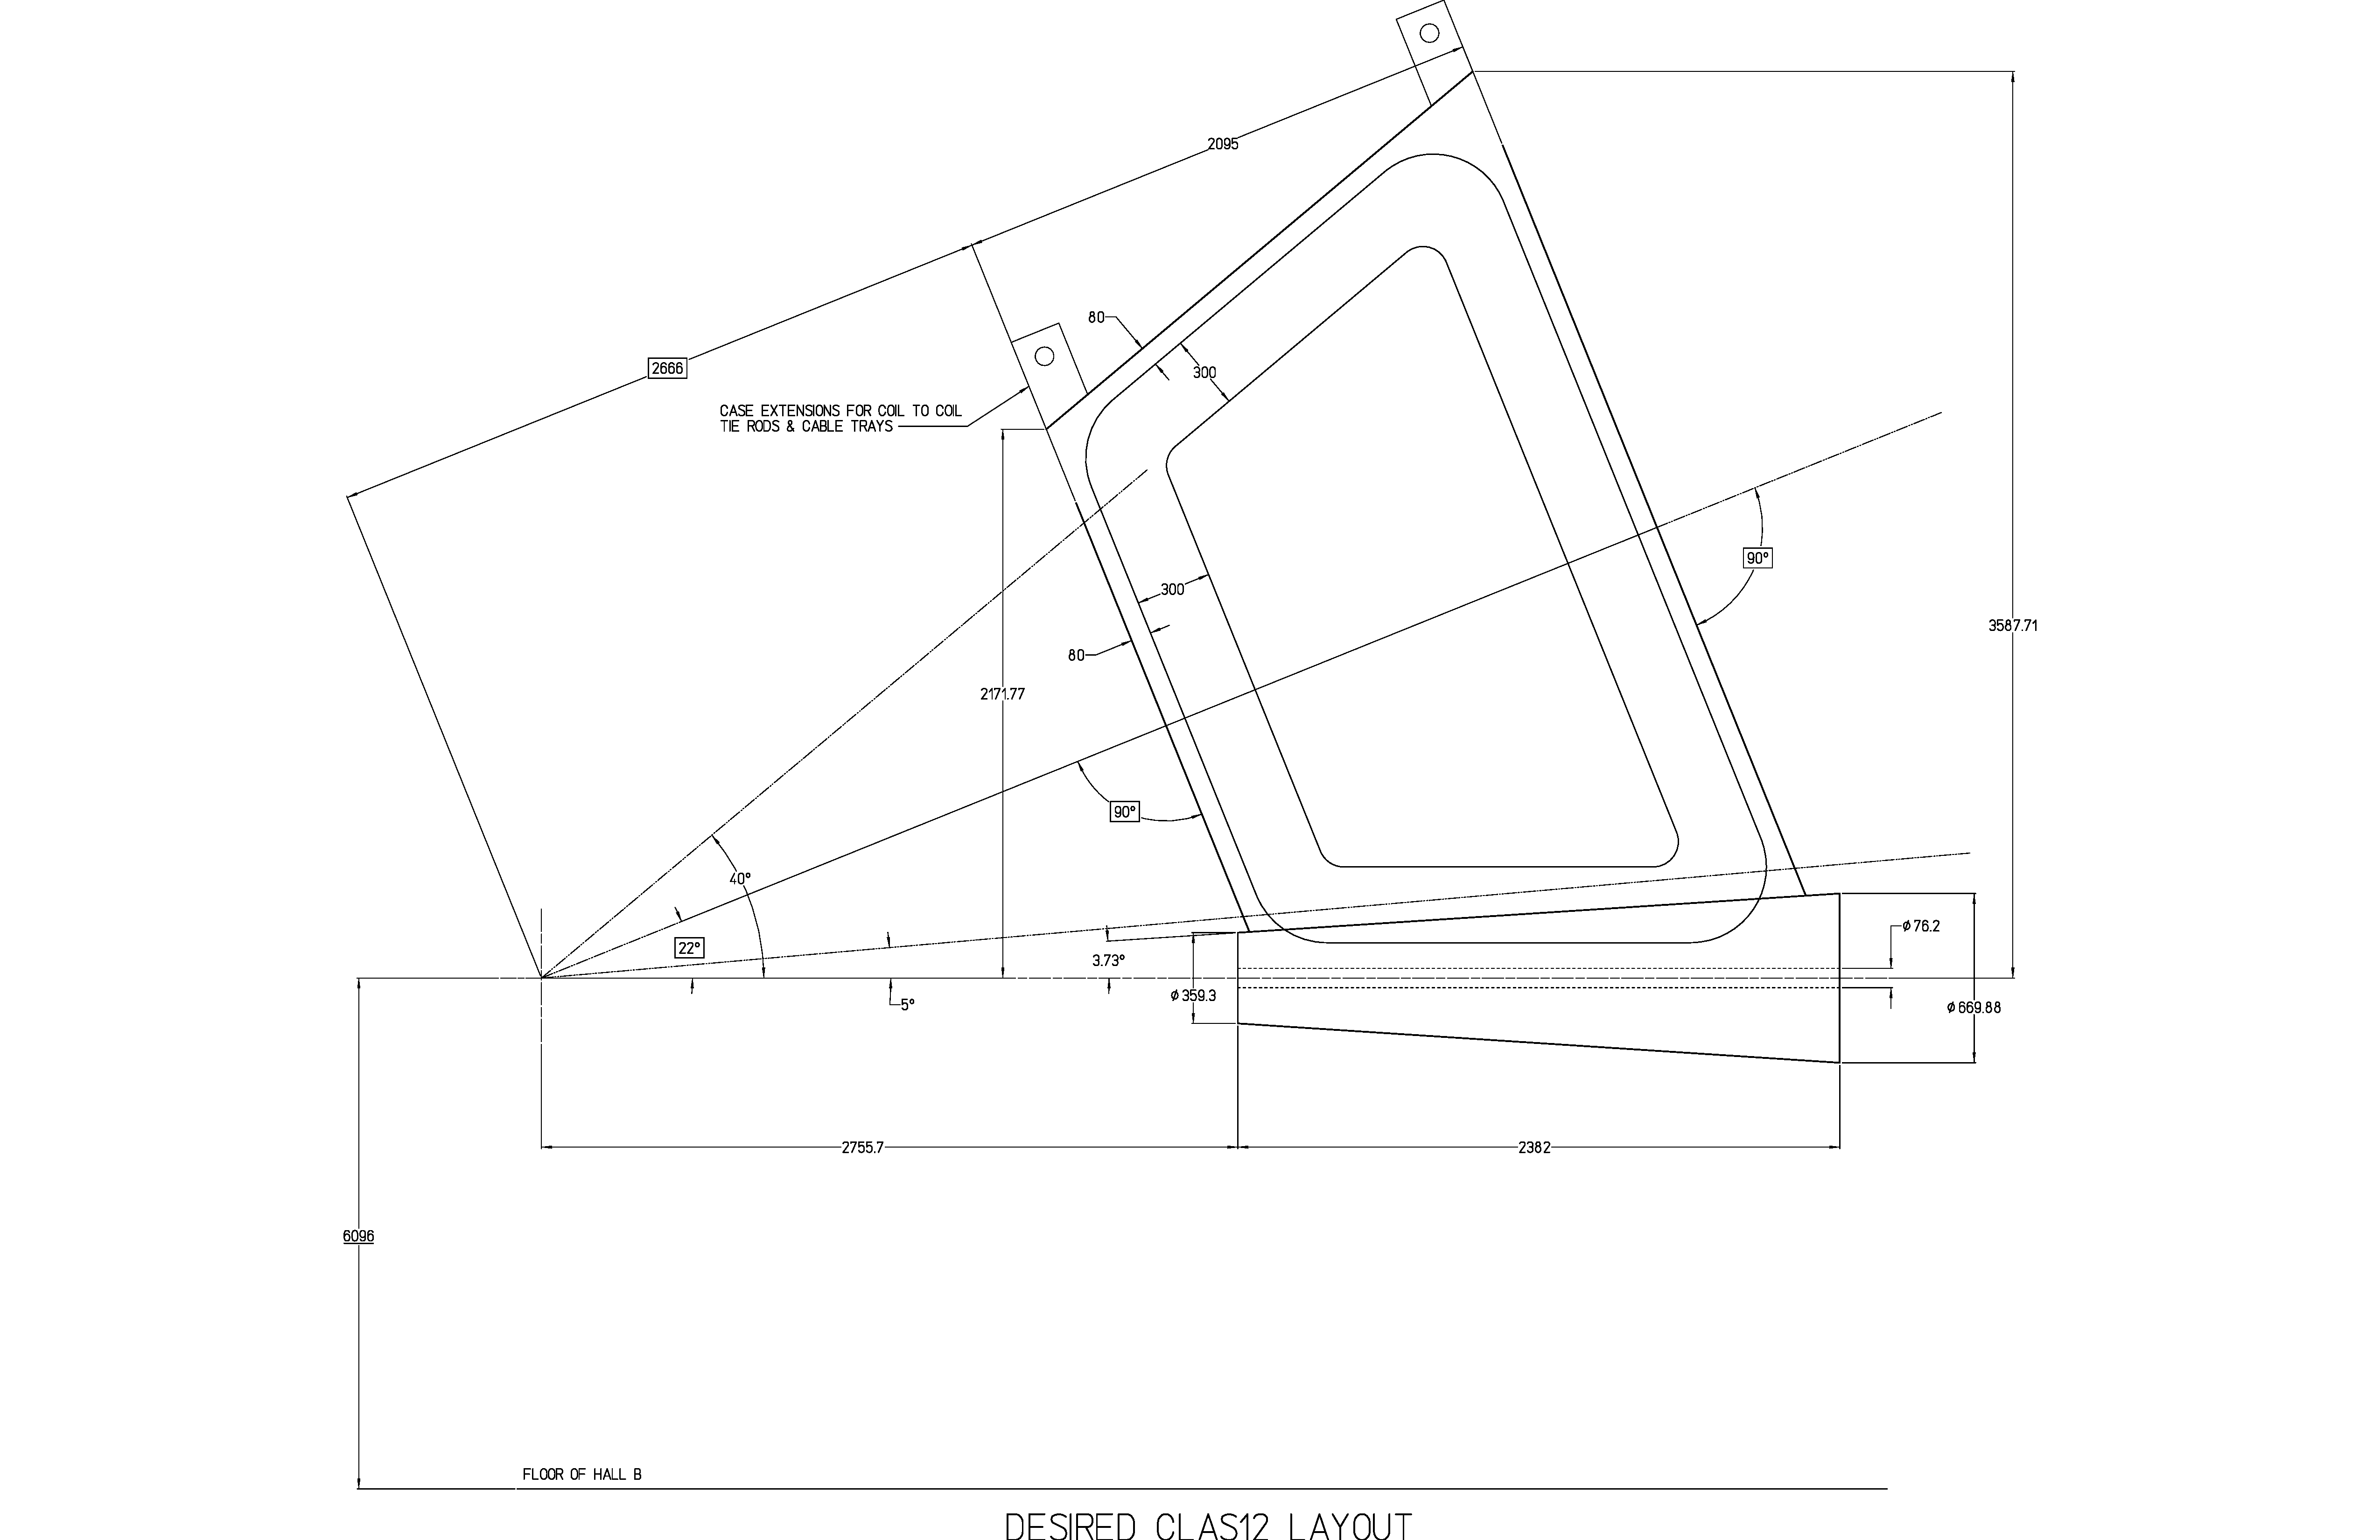
\includegraphics[width=0.16\textwidth,natwidth=610,natheight=642,angle=-90]{clas12_desired.pdf}}}
\end{picture} 
\caption{The shape and dimensions of one of the Torus magnet coils.}
\label{coil-shape}
\end{figure}

\begin{figure}[htbp]
\vspace{4.4cm}
\begin{picture}(50,50)
\put (20,10)
{\hbox{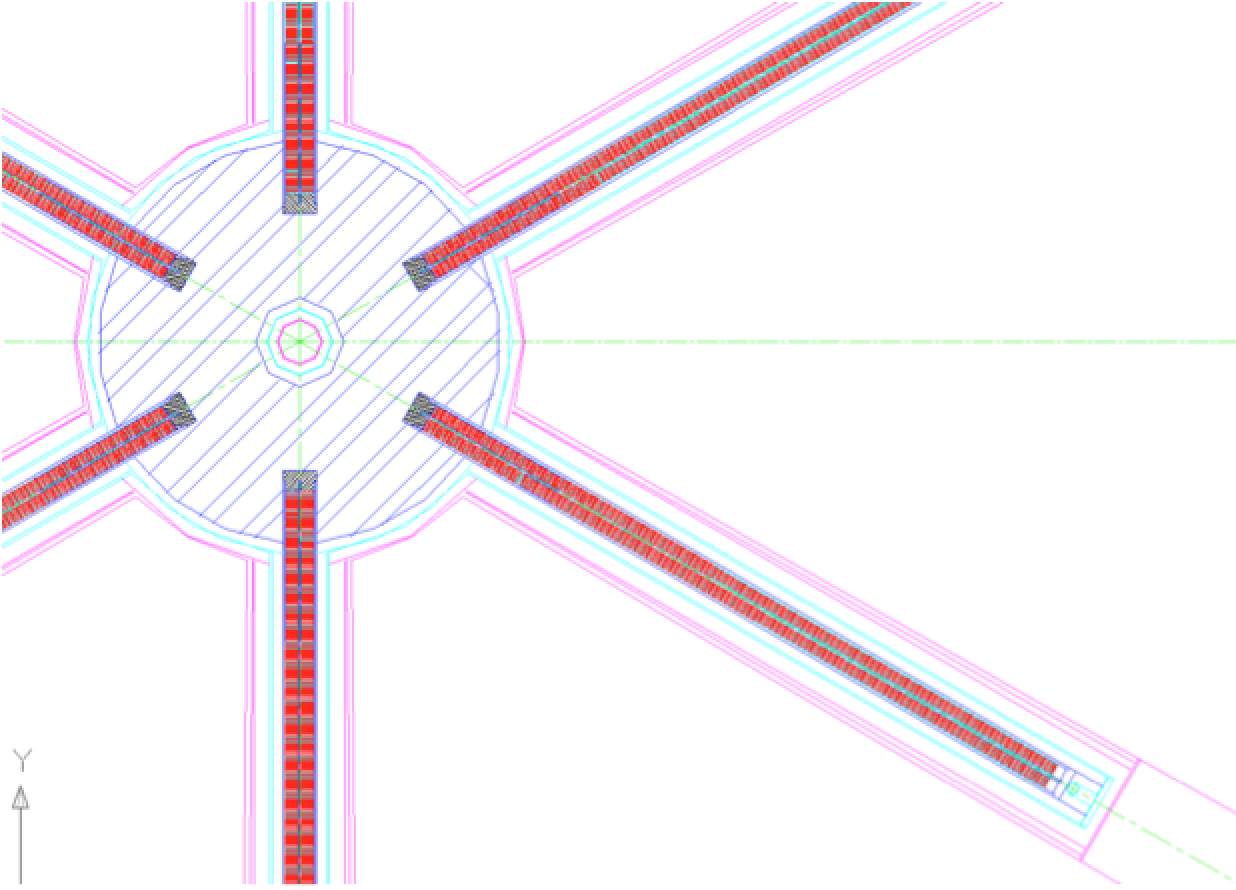
\includegraphics[width=0.28\textwidth,natwidth=610,natheight=642]{coil-mount.png}}}
\end{picture} 
\caption{The six Torus coils are mounted on the cold central stainless steel cone that bears the centripetal force. The
  dark-shaded areas indicate the location of the superconducting coils, surrounded by the cryostat and vacuum jacket.
  {\bf GET MORE DETAILED ENGINEERING DRAWING WITH DIMENSIONS} }
\label{coil-mount}
\end{figure}

\subsection{Forward Detector Tracking System} 

The Forward Detector (FD) has at its core a six-coil superconducting Torus magnet with the individual coils symmetrically
arranged around the beamline within a circle of approximately 7.2~m in diameter. The six coils of the Torus magnet
mechanically support the forward tracking system, which consists of independent drift chamber systems in each of the six
sectors of the Torus magnet. Each of the six drift chamber sectors has a total of 36 layers with 112 sense wires, arranged
in 3 regions (R1, R2, and R3) of 12 layers each. In each of the six Torus sectors the drift chambers are arranged identically.
As displayed in Fig.~\ref{clas12-dc}, the R1 chambers are located at the entrance to the Torus magnetic field region, the R2
chambers are located inside the magnet where the magnetic field is close to maximum, and the R3 chambers are placed in a
low magnetic field space just downstream of the Torus magnet. This arrangement provides independent and redundant tracking
in each of the six Torus sectors. Each of the 3 regions consists of 6 layers with wires strung at $\Delta{\phi} = 84^\circ$ from
the sector mid-plane and 6 layers with wires strung at $\Delta{\phi} = 96^\circ$ from sector mid plane. This stereo view
enables excellent resolution in the most important polar angle (laboratory scattering angle), and good resolution in the less
critical azimuthal scattering angle. Fig.~\ref{dc-stringing} shows the wire stringing operation for the large R3 chambers. 

\begin{figure*}[htbp]
\vspace{6.0cm}
\begin{picture}(50,50)
\put(30,0)
{\hbox{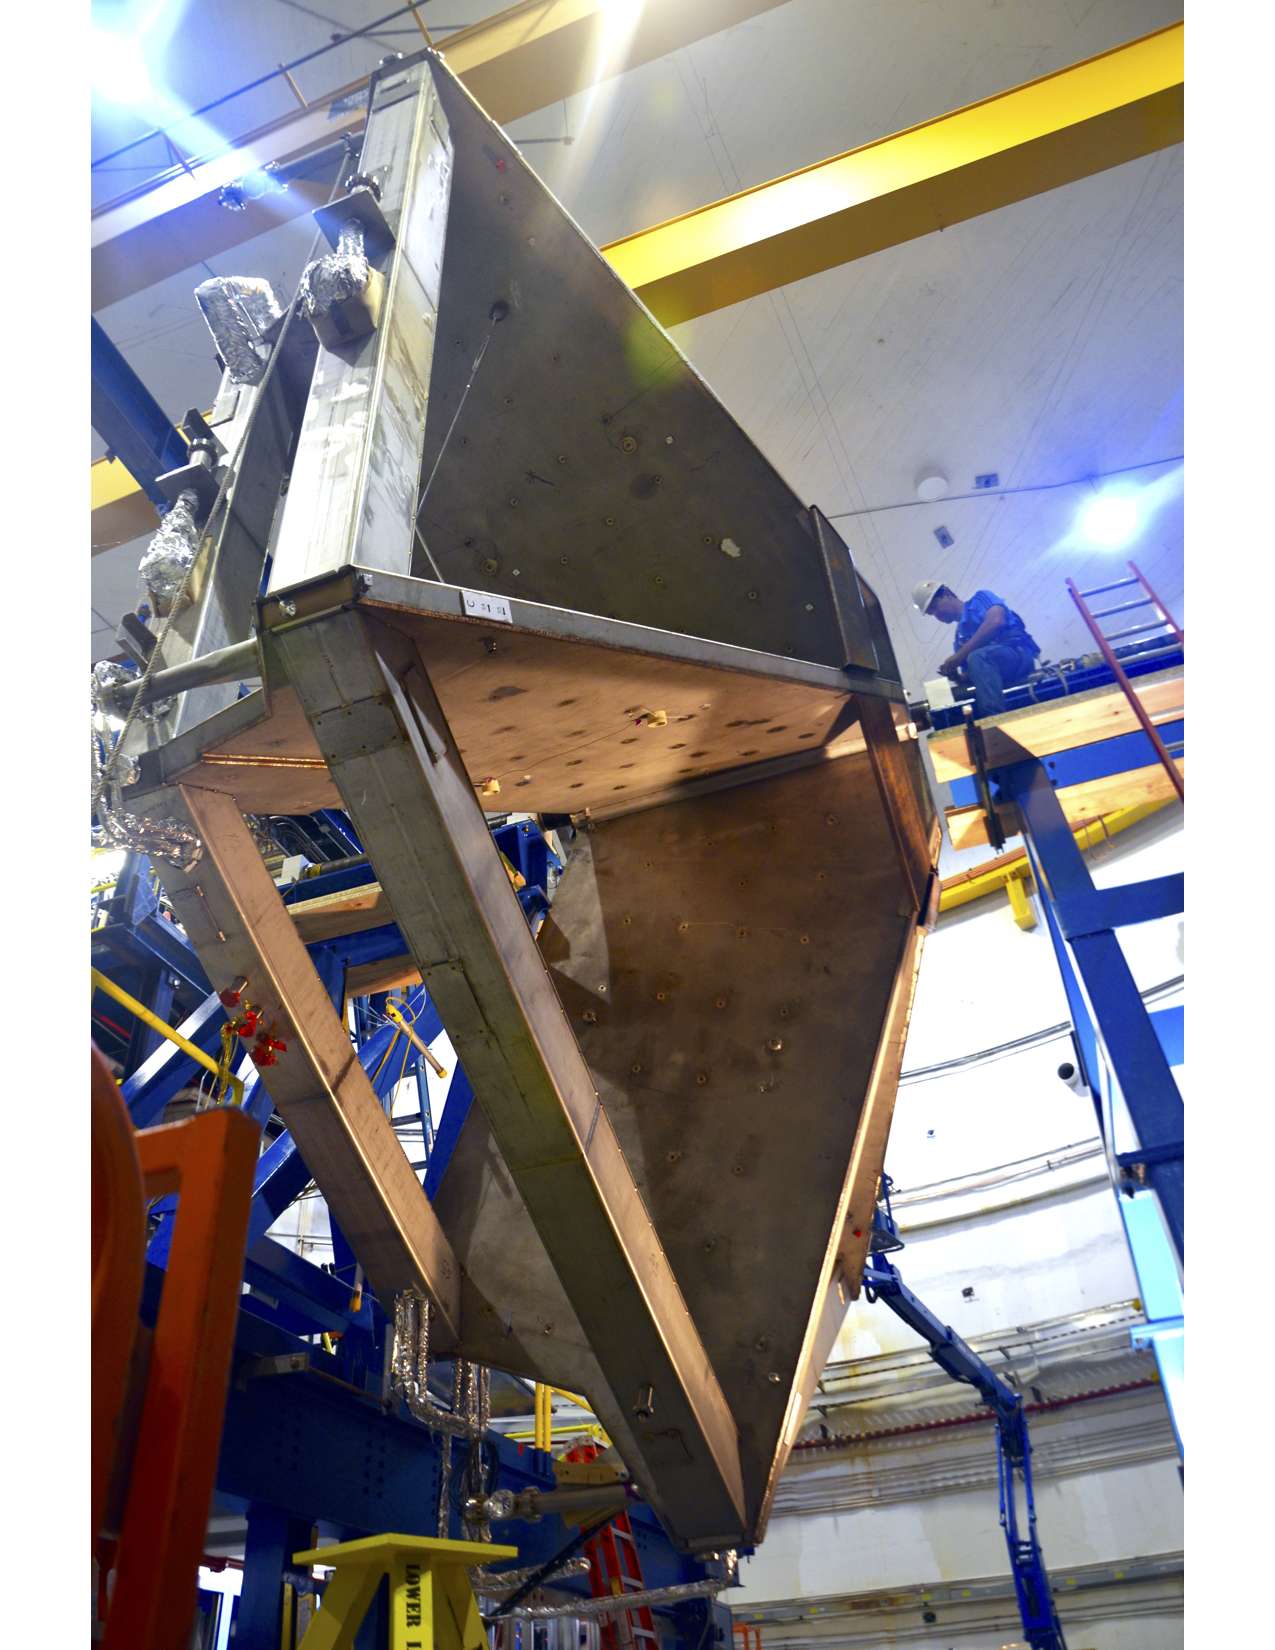
\includegraphics[width=0.27\textwidth,natwidth=610,natheight=642]{Torus-assembled.png}}}
\put(260,0)
{\hbox{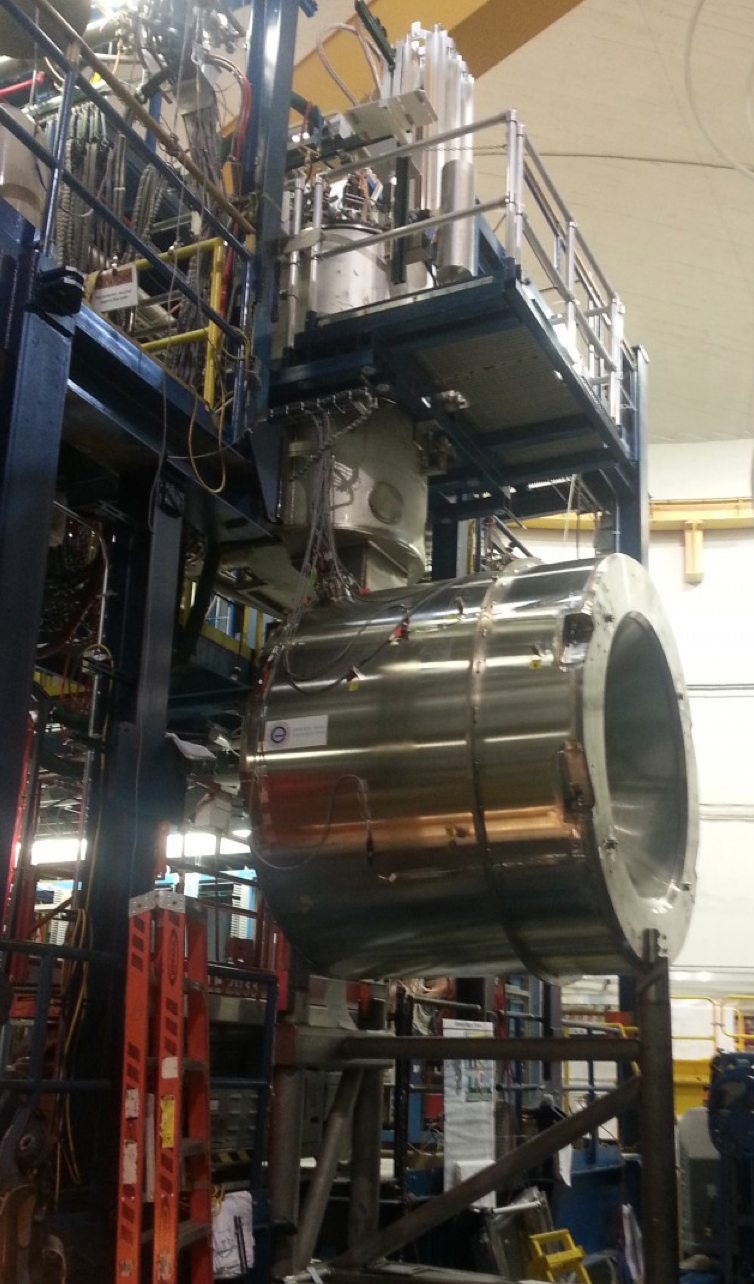
\includegraphics[width=0.35\textwidth,natwidth=610,natheight=642]{solenoid-magnet.png}}}
\end{picture} 
\caption{The CLAS12 magnet system. Left: The Torus magnet with all six coils mechanically assembled in the common
  cryostat. The coil cryostat, which is fabricated from non-magnetic steel, has an outside width of 124~mm. The  cross
  bars provide a cold (5~K) cryogenic connection of neighboring coils, and counteract the out-of-plane forces to provide
  mechanical stability to the full magnet. Due to the large physical size of the assembled Torus magnet, the final assembly
  of the magnet had to be completed in the Hall. Right: The fully assembled Solenoid magnet including all cryogenic
  connections on the beamline at the beginning of cool down, before the detector installation.}
\label{clas12magnets}
\end{figure*}

\subsection{Particle Identification After Tracking}   

Cherenkov counters, time-of-flight detectors,  and electromagnetic calorimeters are located  downstream of the tracking
system to provide particle identification and energy measurements for electrons, high energy photons, and neutrons.
Fig.~\ref{clas12-fd} shows a beam's eye view of the assembled FD, with the six Torus coil cryostats symmetrically
arranged around the beamline. It should be noted that the entire Torus magnet is placed in one hermetic vacuum system,
with the coil cooling provided by cooling tubes soldered to the inner side of the coils.  In the following we briefly describe
the CLAS12 magnet systems. 

\subsection{The Magnet System}
\label{torus}

The contour of one of the six identical coils of the Torus magnet is shown in the  Fig.~\ref{coil-shape}. The geometrical
coverage as seen from the target ranges from $5^\circ$ to $40^\circ$ in polar angle. The symmetrically arranged six
magnet coils provide an approximate toroidal magnetic field around the beamline. The six coils are mounted in the central
cold hub on a common stainless steel cone, which also provides the geometrical symmetry for the alignment of the coils near
the magnet center (see Fig.~\ref{coil-mount}). This guarantees mounting of the coil packages in areas where the magnetic
field is expected to be maximal. A full view of the assembled Torus coils and cryostat is shown in Fig.~\ref{clas12magnets}.
The coverage in azimuthal angle depends on the polar angle of the particle trajectory, and ranges from 50\% of $2\pi$ at
$5^\circ$ to about 90\% of $2\pi$ at $40^\circ$. Each superconducting coil is made from a double-pancake potted in an
aluminum case. The number of windings per pancake is 117. The conductor is SSC outer dipole cable soldered into a
20~mm$\times$2.5~mm copper channel with a turn-to-turn insulation of 75~$\mu$m fiber-glass tape. Operating at a nominal
current of 3770~A, the peak field is 3.58~T at the inner turns close to the warm bore. For symmetry reasons the field on the
beam axis is ideally equal zero, with a small remnant field present due to imperfections in the magnet assembly and location.
The $\int {Bdl}$ at the nominal current is 2.78~Tm at $5^\circ$ and 0.54~Tm at $40^\circ$. The inductance of the magnet is
2.0~H and the stored energy 14.2~MJ. The magnet has liquid $N_2$ cooled heat shields. After assembly and cool down, the
magnet reached full field immediately.  (For details on the design and operation of the Torus magnet, see
Ref.~\cite{clas12-magnets}.)

\begin{figure}[htbp]
\vspace{4.2cm}
\begin{picture}(50,50)
\put(8,0)
{\hbox{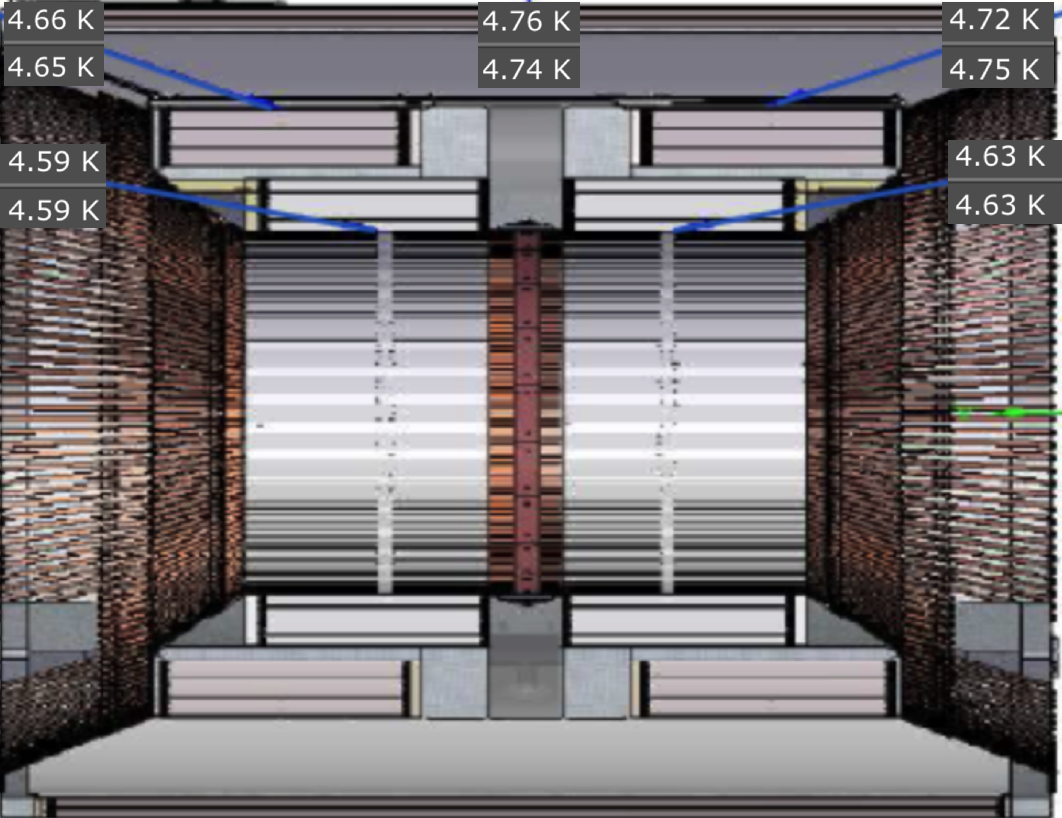
\includegraphics[width=0.35\textwidth,natwidth=610,natheight=642]{solenoid-coils.png}}}
\end{picture} 
\caption{The solenoid coils with the $2 \times 2$ main coils on the inside, and the shield coil on the outside. The numbers
  indicate the respective temperatures for each coil after cool down, on average 4.65~K. }
\label{solenoid-coils}
\end{figure}

\begin{figure}[htbp]
\vspace{7.0cm}
\begin{picture}(50,50)
\put(25,-10)
{\hbox{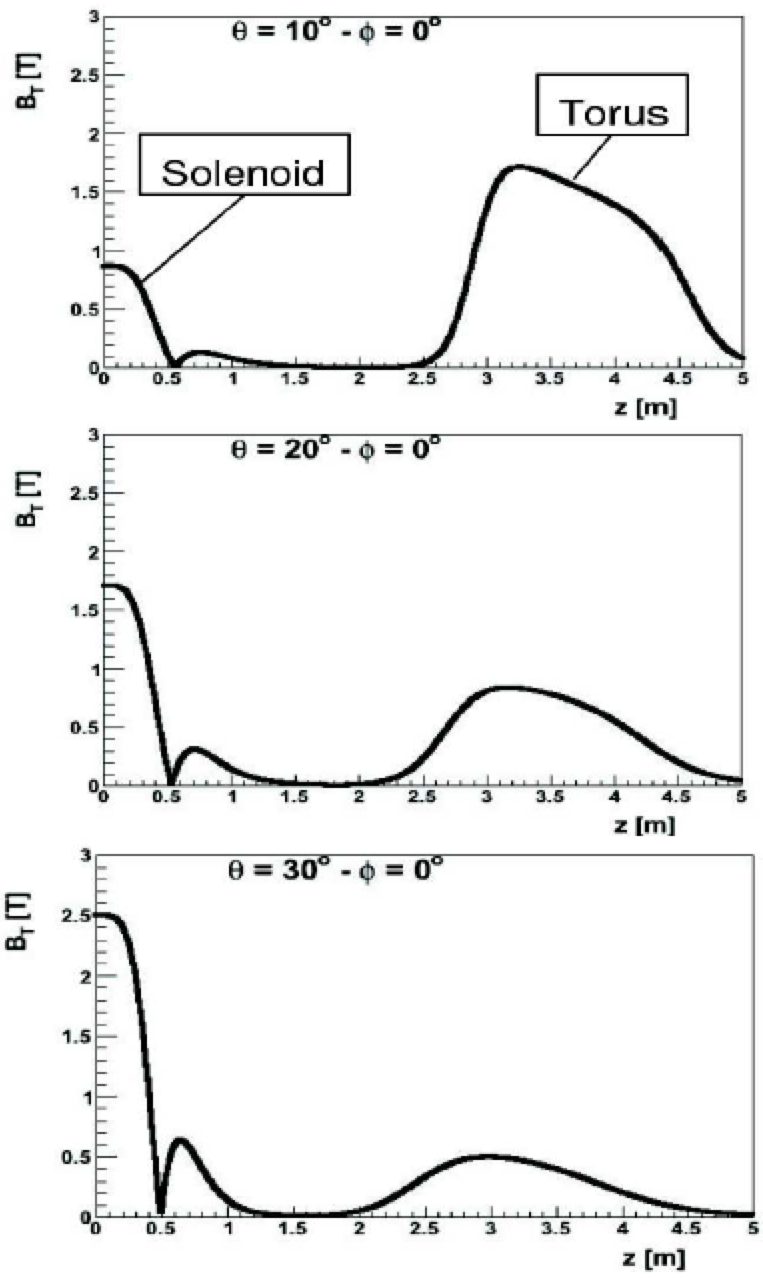
\includegraphics[width=0.40\textwidth,natwidth=610,natheight=642]{magfield.png}}}
\end{picture} 
\caption{Combined Solenoid and Torus magnetic fields,  showing the total transverse magnetic field along the radial
  distance from the Solenoid center. The two magnetic fields act differently on charged particles. Only the transverse
  components act on the charged tracks and depends on its orientation relative to the momentum vector of the charged
  particle.  With increasing polar angles as seen from the Solenoid center, the transverse components increase in the
  Solenoid, while they decrease in the Torus magnet.}
\label{solenoid-torus}
\end{figure}

\begin{figure}[htbp]
\vspace{6.0cm}
\begin{picture}(50,50)
\put(10,0)
{\hbox{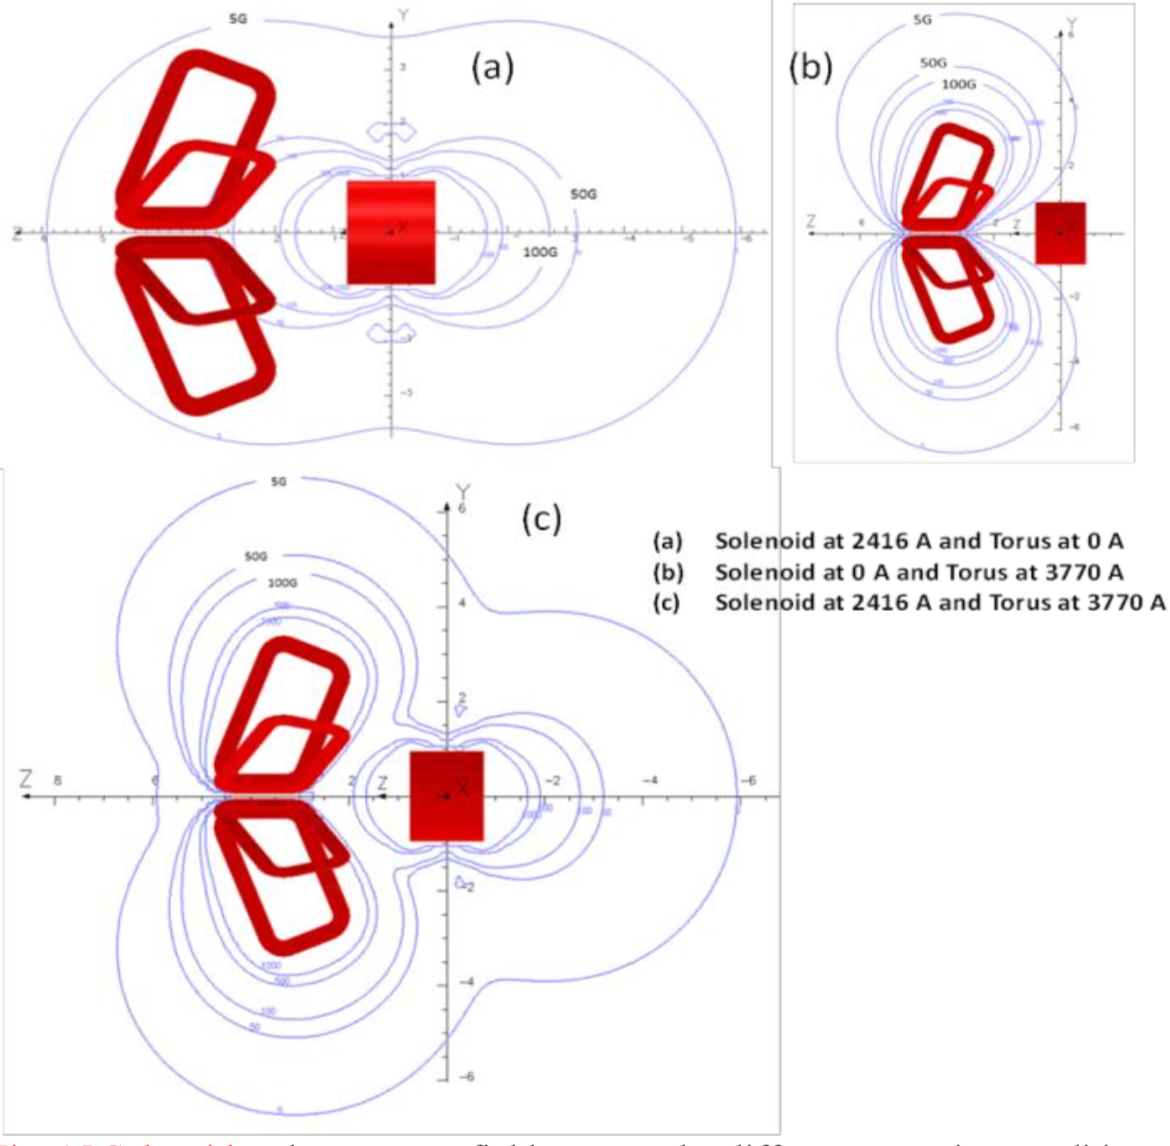
\includegraphics[width=0.32\textwidth,natwidth=610,natheight=642]{Torus-Solenoid-stray-field.png}}}
\end{picture} 
\caption{Solenoid and Torus magnetic stray fields, individually (a) and (b), and combined (c). {\bf GET SHARPER GRAPHS
  FROM MAGNET GROUP.}}
\label{stray-field}
\end{figure}

The stray magnetic field of the combined superconducting Solenoid and Torus magnets are shown in Fig.~\ref{stray-field}. 

\begin{figure}[htbp]
\vspace{7.0cm}
\begin{picture}(50,50)
\put(65,105)
{\hbox{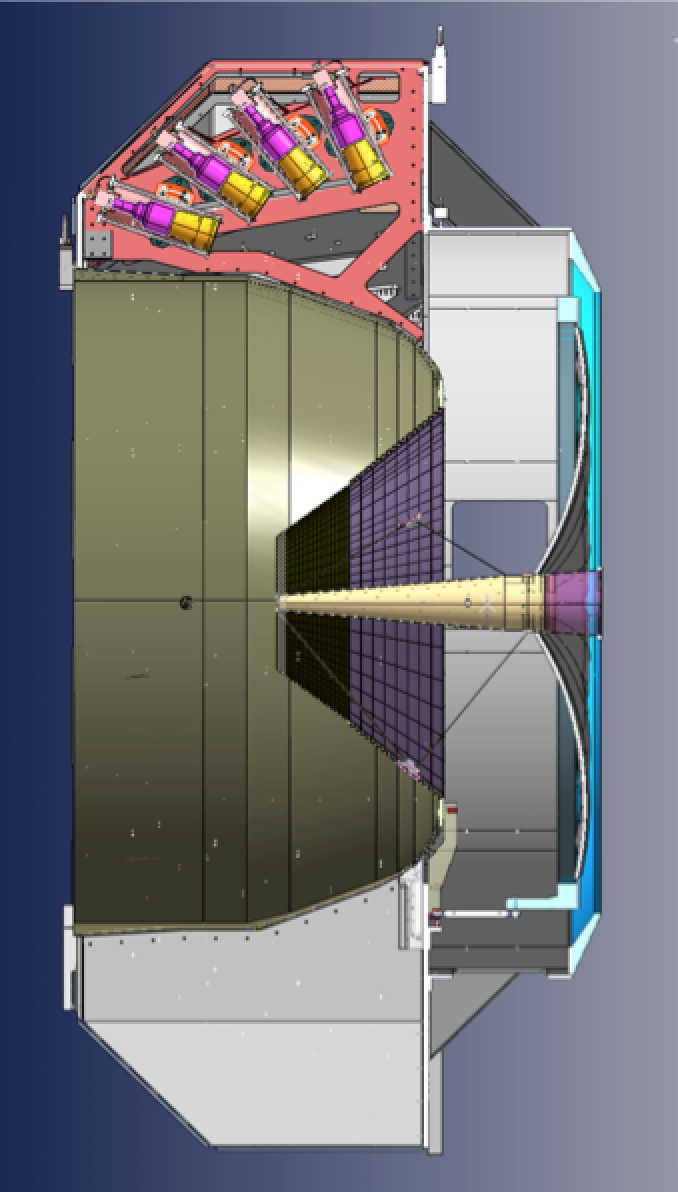
\includegraphics[width=0.28\textwidth,natwidth=610,natheight=642]{CLAS12-HTCC.png}}}
\put(45,-5)
{\hbox{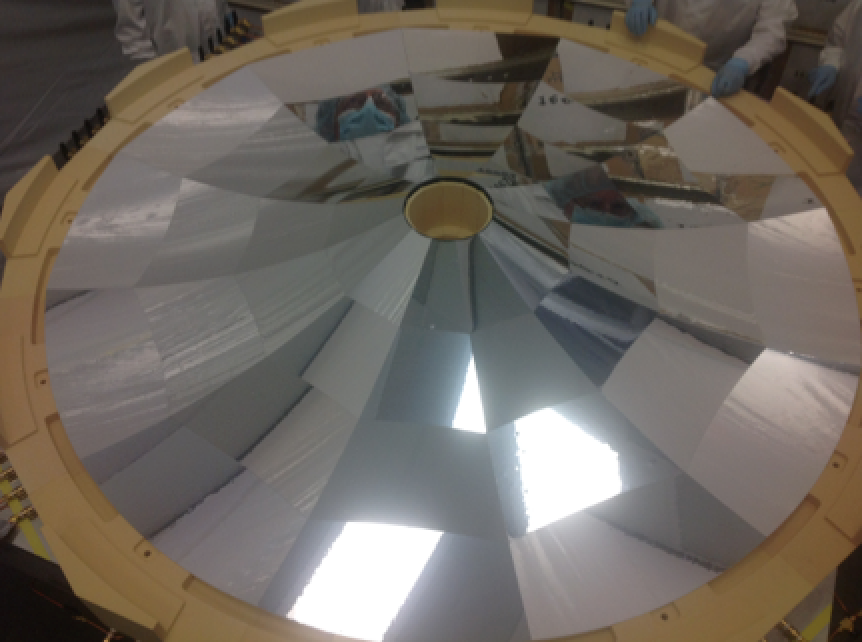
\includegraphics[width=0.30\textwidth,natwidth=610,natheight=642]{HTCC-mirror.png}}}
\end{picture} 
\caption{Top: Design model rendering of the HTCC detector in a side cut. The beam enters from the left. Bottom: The
  HTCC mirror with its 48 mirror facets, each reflecting the Cherenkov light to a different photomultiplier
  tube. The mirror is about 3~m in diameter.}
\label{htcc}
\end{figure}

\begin{figure}[htbp!]
\vspace{5.0cm}
\begin{picture}(50,50)
\put(35,0)
{\hbox{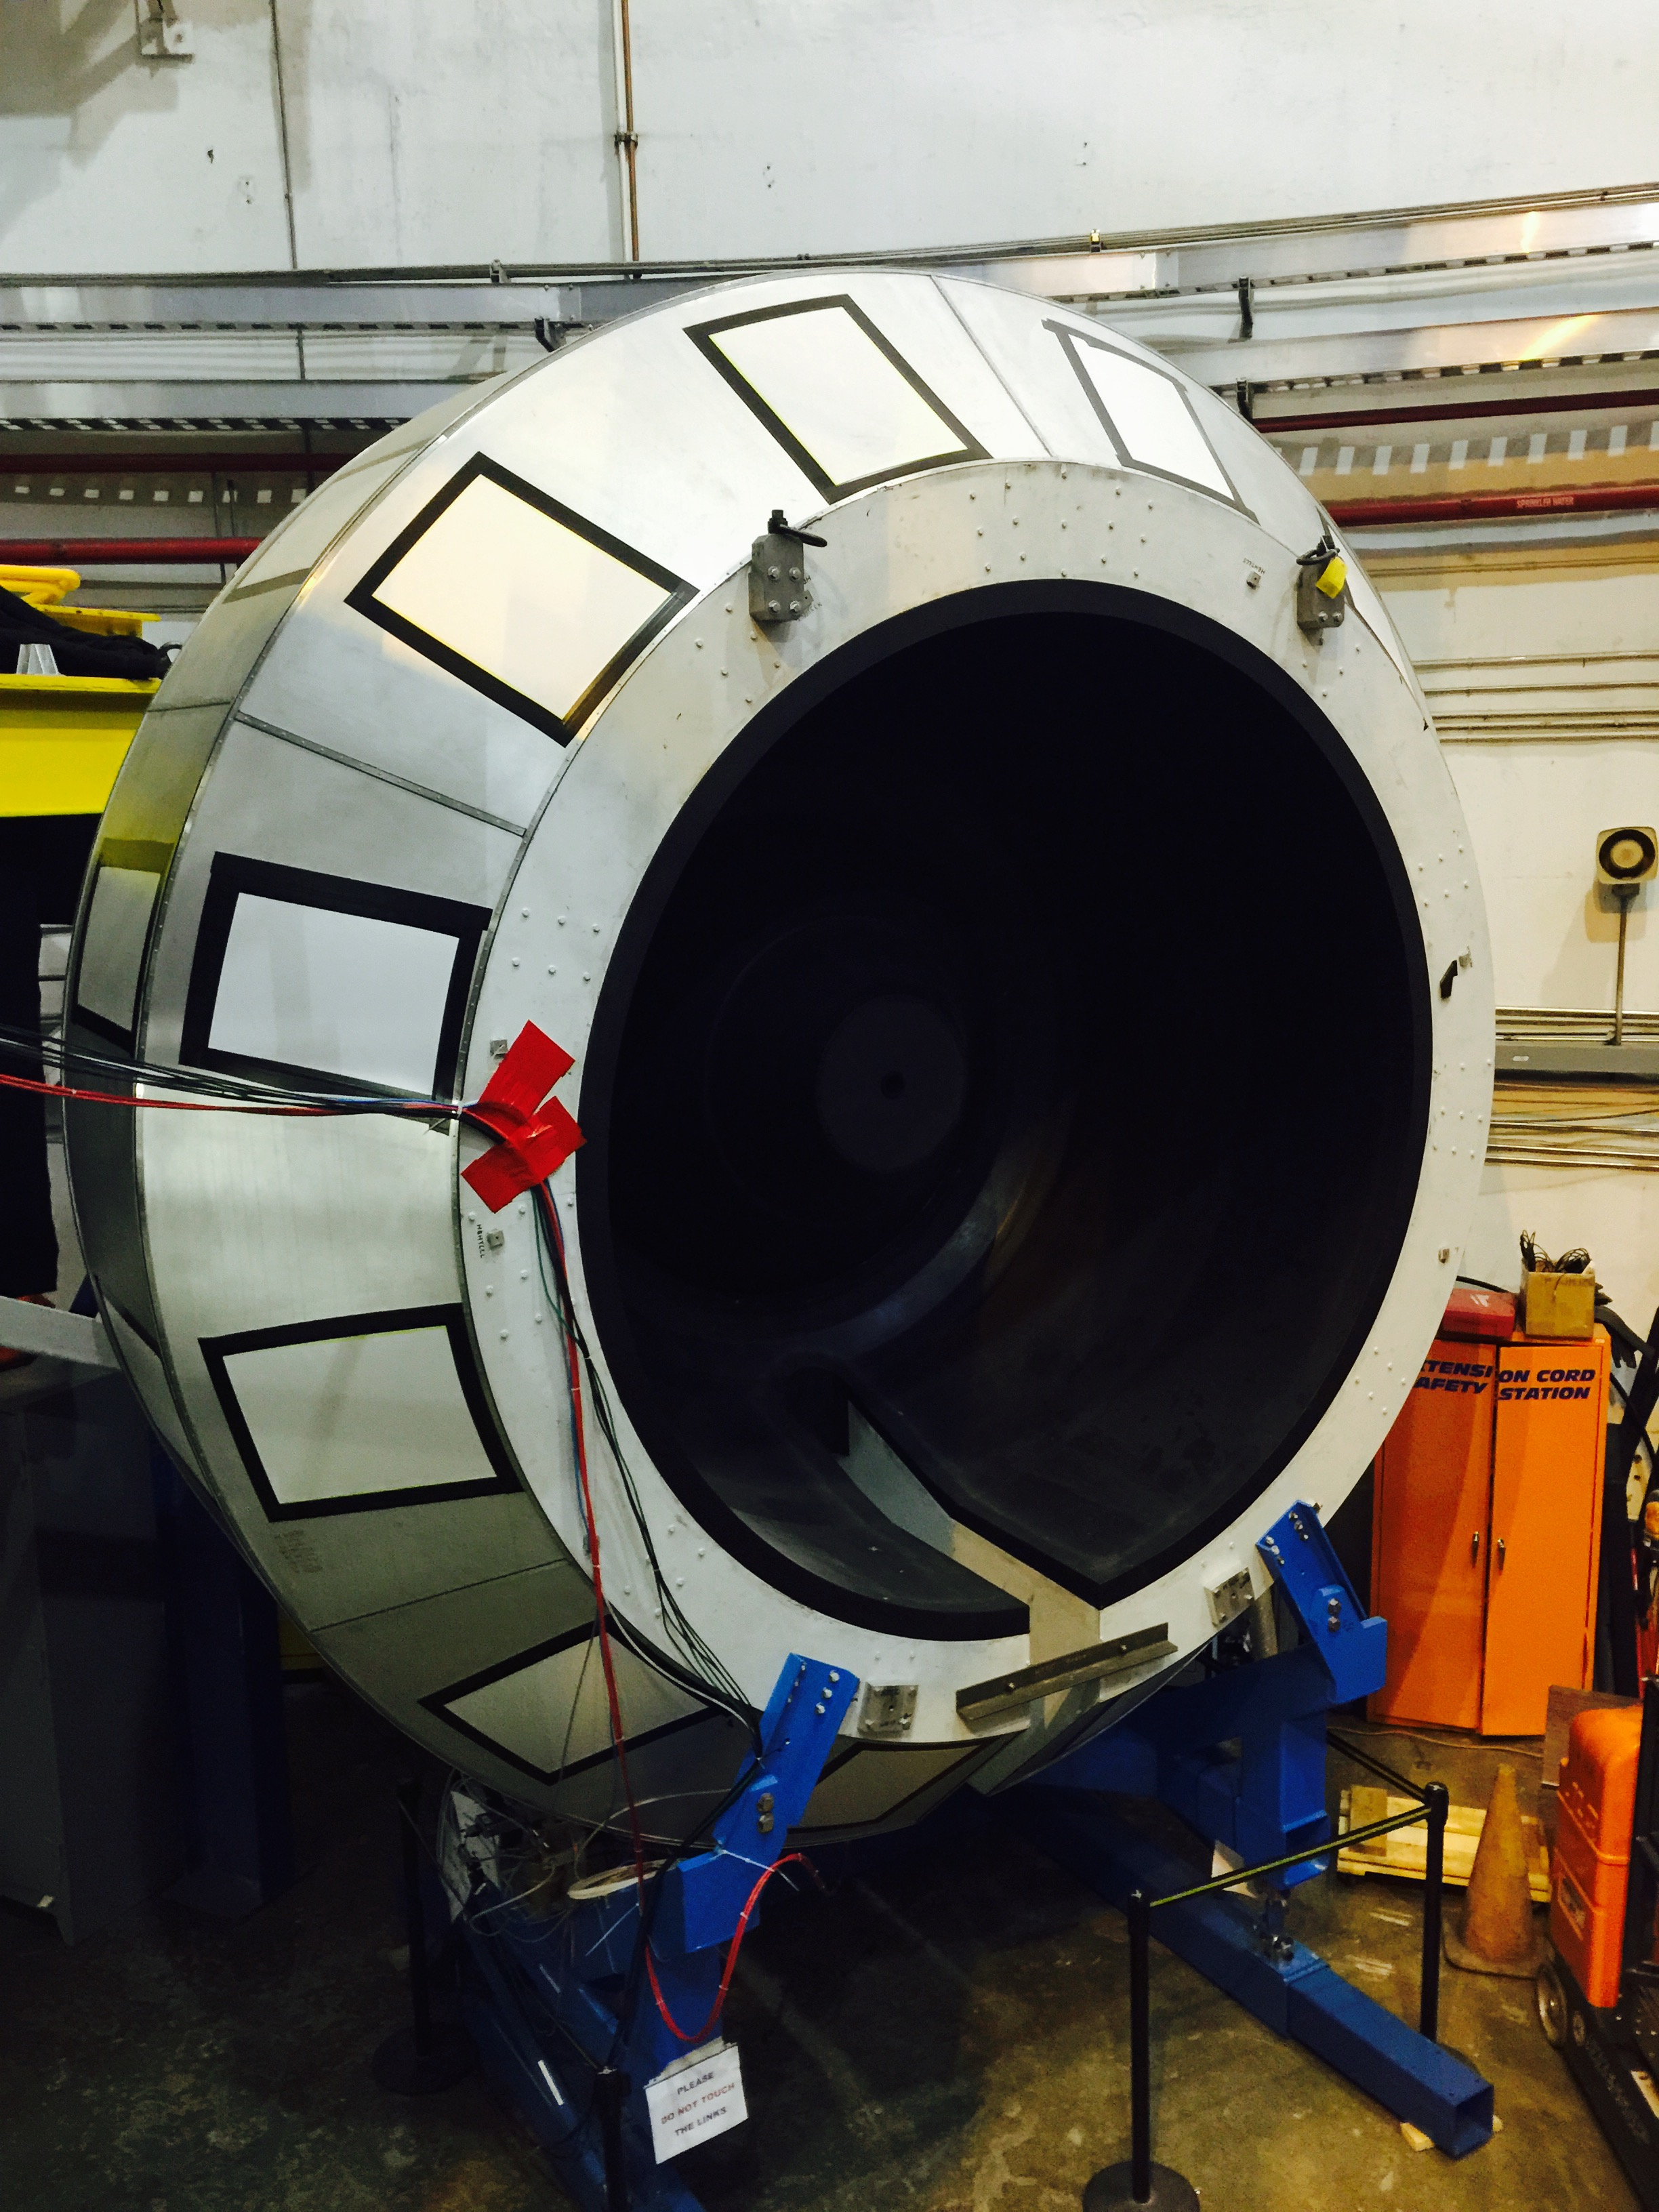
\includegraphics[width=0.12\textwidth,natwidth=610,natheight=642]{HTCC.jpg}}}
\end{picture}  
\caption{Fully assembled HTCC detector before its installation in the Hall~B beamline. The container spans about 5~m in
  diameter.  {\bf Check this number!}}
\label{HTCC-container}
\end{figure}

The Solenoid magnet is a self-shielded superconducting magnet around the beamline used to generate a field primarily in
the beam direction. The fully assembled magnet is displayed in Fig.~\ref{clas12magnets}, and Fig.~\ref{solenoid-coils}
shows the solenoid coils design layout. The design is driven by the physics requirements to (a) provide a magnetic field for
particle tracking at large angles, (b) act as M\"oller electron shield, and (c) provide a highly uniform field at the magnet
center for the operation of dynamically polarized proton and deuteron targets. The magnet consists of 4 cylindrical coils
arranged in two packages at different radial distances to the beamline. The 5th coil is located outside of the 4 inner coils
and generates a magnetic field that compensates the field of the 4 inner coils and thus acts as an active magnetic shield.
The number of turns in the main coils is 3704 $(2 \times 840 + 2 \times 1012)$, and in the shield coil 1392. The magnet is
powered at a nominal currents of 2416~A. The integrated field length along the magnet center is $\int Bdl = 7.0$~Tm,
generating a stored energy of 20~MJ.  At full current the solenoid generates a 5~T magnetic field at its center. The magnet
has an inner warm bore of 78~cm diameter where all the central detectors are placed.  For details on the design and operation
of the Solenoid magnet, see Ref.~\cite{clas12-magnets}. The distribution of the absolute magnetic field along lines of constant
polar angles seen from the target position is shown in Fig.~\ref{solenoid-torus}. Both, the Torus and Solenoid magnetic fields
are included. For details of the CLAS12 Solenoid magnet see~Ref. \cite{clas12-magnets}. 

\begin{figure}[htbp]
\vspace{4.5cm}
\begin{picture}(50,50)
\put(25,-5)
{\hbox{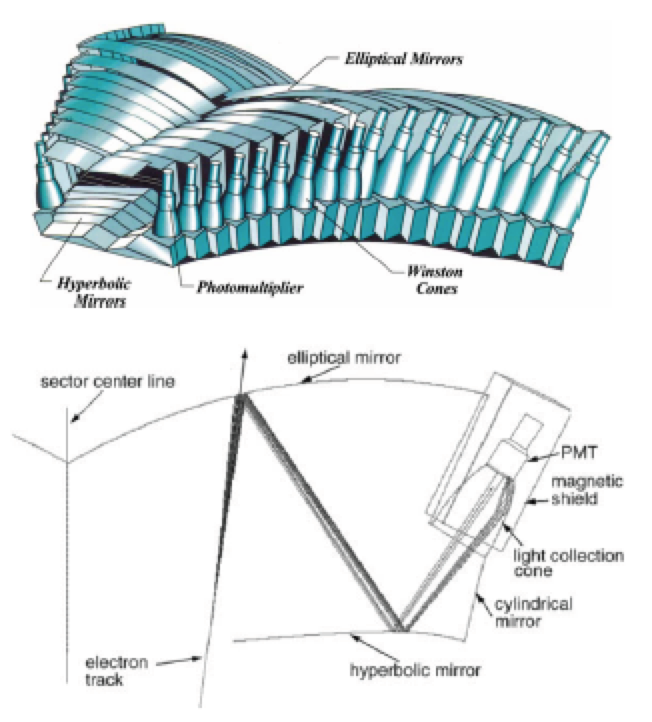
\includegraphics[width=0.50\textwidth,natwidth=610,natheight=642]{ltcc.png}}}
\end{picture} 
\caption{The LTCC detector. Top: Rendering of the mirror system in 3D. Bottom: 2D representation of the optical
  system. The large acceptance coverage requires a complex mirror system for efficient light collection.{\bf GET
  SHARPER DRAWINGS} }
\label{ltcc}
\end{figure}

\subsection{High Threshold Cherenkov Counter (HTCC)}
\label{}

The HTCC is operated with dry CO$_2$ gas at 1 atm gas pressure, and is the main detector to separate electrons (positrons)
with momenta below 4.9~GeV from charged pions, kaons and protons. The detector has full coverage of 360$^\circ$ in azimuth
and spans from 5$^\circ$ to 35$^\circ$ in polar angles. It has no blind areas in complete solid angle covered. The detector is
located downstream of the production target, sandwiched between the Solenoid magnet and the Torus magnet, in front of the
forward tracking detectors. In order to minimize multiple scattering in the HTCC detector materials, e.g. the mirror system
with its backing structure, and to limit its impact on the momentum analysis of charged tracks in the Torus field, the HTCC
mirror system is constructed from low-density composite material as backing structure. The amount of solid material seen by
charged particles passing through is 135~mg/cm$^2$. The HTCC is one unit with a multi-focal mirror of 60 elliptical mirror
facets that focus the Cherenkov light on 48 phototubes with quartz windows of 125-mm diameter. The phototubes are located in
a magnetic field of up to 35~G oriented along the phototube axes and are covered with a multi-layer magnetic shield and active
compensation coils. The system is required to provide high rejection of charged pions and low background noise for reliable 
identification of scattered electrons in a dense electromagnetic background environment. 

\begin{figure*}[htbp]
\vspace{7.0cm}
\begin{picture}(50,50)
\put(80,90)
{\hbox{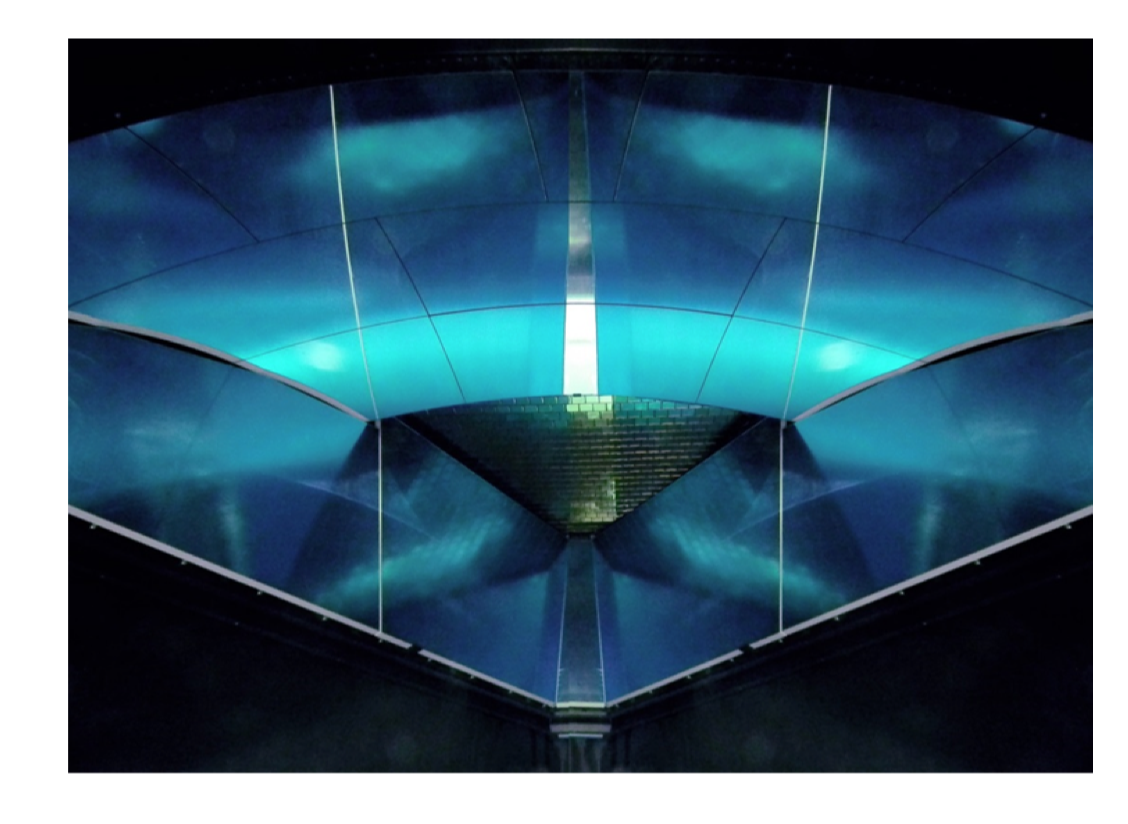
\includegraphics[width=0.45\textwidth,natwidth=610,natheight=642]{rich-mirrors.png}}}
\put(60,-10)
{\hbox{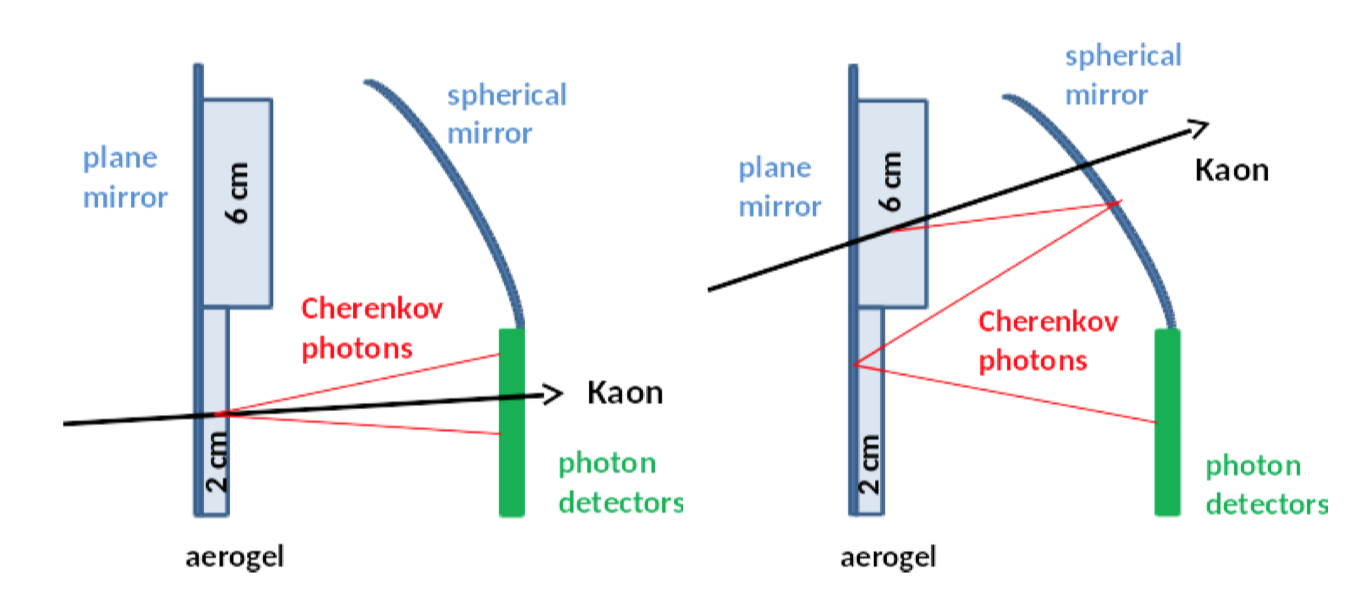
\includegraphics[width=0.45\textwidth,natwidth=610,natheight=642]{rich.png}}}
\end{picture} 
\caption{The RICH detector. Top panel: Mirror system as seen from the entrance window, with the spherical mirrors
  above, and the planar mirrors below. The PMT detector plane is seen in the center. Bottom panel: The principle operation
  of operation the RICH detector and its internal optics for direct photon and reflected photon detection. }
\label{rich}
\end{figure*}

The HTCC is also used to generate a fast signal to be used as a trigger for scattered electrons. The HTCC operates in
conjunction with energy deposited in the electromagnetic calorimeters to identify electrons of specific energies. The
HTCC detector container and the $360^\circ$ mirror system are displayed in Fig.~\ref{htcc}.  Fig.~\ref{HTCC-container}
shows a photo of the full detector before installation on the beamline. For details of the HTCC construction and performance,
see Ref. ~\cite{HTCC}.   

\begin{figure*}[htbp]
\vspace{5.0cm}
\begin{picture}(50,50)
\put(5,0)
{\hbox{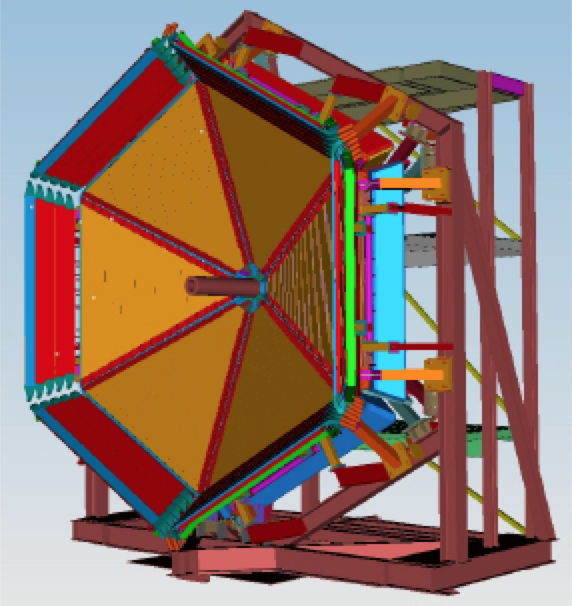
\includegraphics[width=0.65\textwidth,natwidth=610,natheight=642]{CLAS12-FTOF.png}}}
\put (220,0)
{\hbox{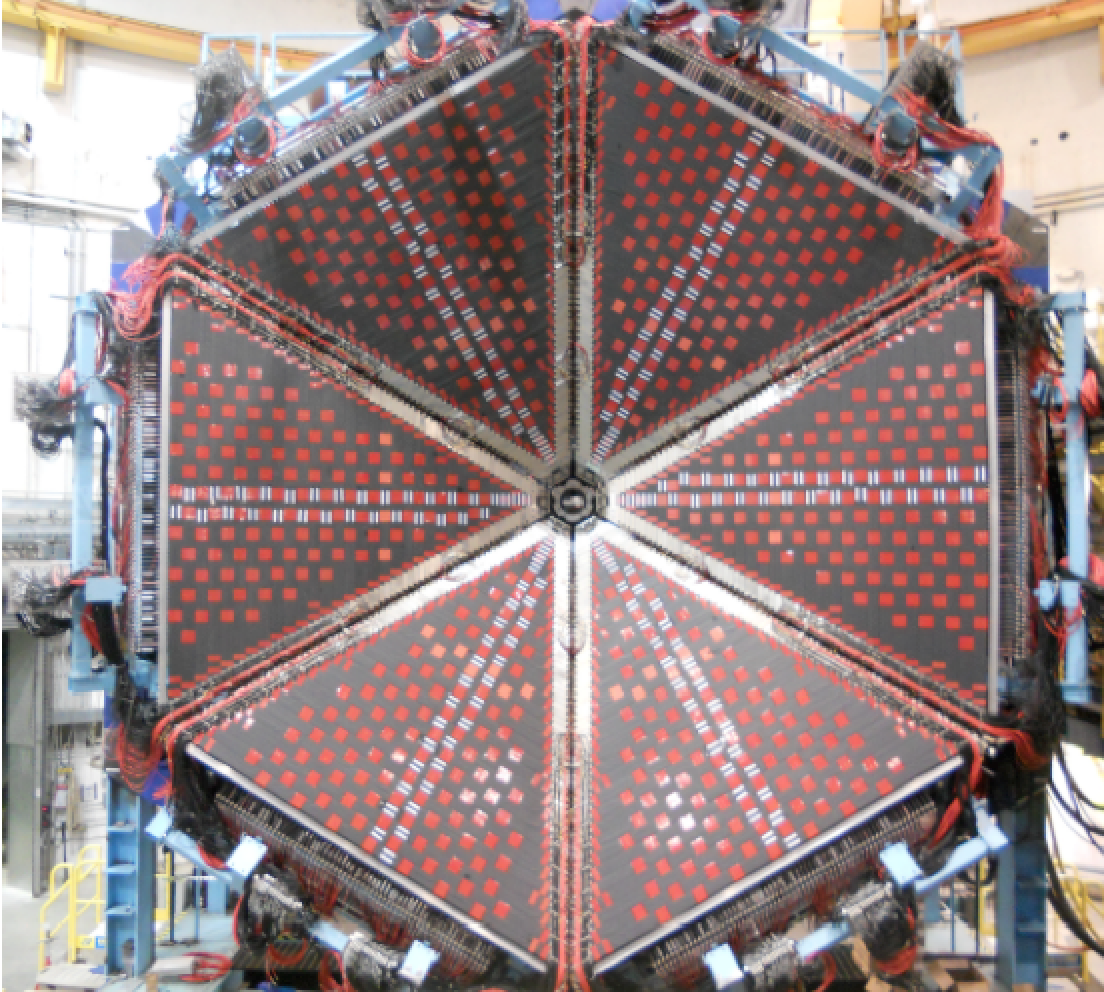
\includegraphics[width=0.40\textwidth,natwidth=610,natheight=642]{FTOF-1b.png}}}
\end{picture} 
\caption{Left: 3D rendering of the FTOF system showing the panels-1b on the inside, and panel-2 on the outside. The
  panel-1a counters are located immediately downstream of the panel-1b counters and are not visible here. Right: FTOF
  panel-1b counters mounted on the CLAS12 Forward Carriage in front of panel-1a and PCAL.} 
\label{ftof-1b}
\end{figure*}

\subsection{Low Threshold Cherenkov Counters (LTCC)}

The LTCC system is part of the CLAS12  Forward Detector and is used for charged pion and kaon discrimination 
at momenta greater than 3.5~GeV. The LTCC system consists of boxes shaped like truncated pyramids. Four 
of the six sectors of CLAS12 are equipped with one LTCC box each. Each LTCC box contains 108 light-weight 
mirrors with composite backing structure, 36 Winston light-collecting cones , 36 125~mm diameter photomultiplier tubes,
and 36 magnetic shields. The LTCC boxes are filled with heavy C$_4$F$_{10}$ radiator gas, providing pion discrimination 
from kaons for momenta of 3.5 to 9~GeV.  The LTCC system has previously been used to detect electrons in the CLAS
detector at lower energies~\cite{Adams:2001kk}. It has been refurbished to provide higher efficiency for charged pion
detection by increasing the volume of the radiator gas, refurbishing the elliptical and hyperbolic mirrors with new coating,
and improving the sensitivity of the phototubes to Cherenkov light by coating their entrance windows with wavelength shifting
material that absorbs UV light at wavelength below 300~nm and re-emits two back-to-back photons at larger wavelength. A
rendering of the LTCC mirror arrangement and the principles of the optical system are shown in Fig.~\ref{ltcc}.  For details
of the LTCC construction, the detector refurbishments, and its performance, see Ref.~\cite{LTCC}.   

\subsection{Ring Imaging Cherenkov Detector (RICH)} 

Some experiments require the detection and identification of charged kaons in momentum ranges that are not accessible
with the standard time-flight method used with the FTOF scintillators, or with the LTCC Cherenkov counters. The
time-of-flight resolution of the scintillators is no longer sufficient, and the threshold of the LTCC is too high to detect
and separate kaons from protons in the momentum range from 3 to 8~GeV. For that purpose an additional RICH detector
was built and incorporated in one of the CLAS12 sectors to replace the corresponding LTCC sector. The RICH detector is
designed to improve CLAS12 particle identification in the momentum range 3-8~GeV. It incorporates aerogel radiators,
visible light photon detectors, and a focusing mirror system that is used to reduce the detection area instrumented by
photon detectors to ~1 m$^2$.  Multi-anode photomultiplier tubes (MA-PMTs) provide the required spatial resolution and
match the aerogel Cherenkov light spectrum in the visible and near-UV region. For forward scattered particles
($\theta < 13^\circ$) with momenta 3 - 8~GeV, a proximity imaging method with thin (2~cm) aerogel and direct Cherenkov
light detection is used. For larger incident particle angles of $13^\circ < \theta < 25^\circ$ and momenta of 3 - 6~GeV, the
Cherenkov light will be produced by a thicker aerogel layer of 6~cm thickness, focused by a spherical mirror, undergo two
further passes through the thin radiator material and a reflection from planar mirrors before detection. Fig.~\ref{rich}
shows the mirror system and the optics of the detector. For details of the RICH detector construction and performance,
see Ref.~\cite{RICH}.

\subsection{Forward Time-of-Flight Counters (FTOF)}
\label{ftof}

The FTOF system is part of the Forward Detector and is used to measure the time-of-flight of charged particles 
emerging from the production target during beam operation. It includes six sectors of plastic scintillators with 
double-sided PMT readout. Each sector consists of three arrays of counters. 
\begin{itemize}
\item Panel-1a - 23 counters 
\item Panel-1b - 62 counters
\item Panel-2 - 5 counters 
\end{itemize}
The system is required for excellent timing resolution for particle identification and good segmentation for 
flexible trigger options. The detectors cover a  range in polar angle from $5^\circ$ to $35^\circ$, and 50\% in $\phi$ at 
$5^\circ$ and 90\% at $35^\circ$. The lengths of the counters ranges from 32.3~cm to 376.1~cm in panel 1a, from~17.3~cm 
to 407.9~cm in panel-1b, and from 371.3~cm to 426.2~cm in panel-2.  The average timing resolution in panel-1a is 120~ps, 
85~ps in panel-1b, and 155~ps in panel-2.  Fig.~\ref{ftof-1b} shows the FTOF system on the Forward carriage.
For details of the FTOF construction and performance, see Ref. ~\cite{FTOF}. 

\begin{figure}[htbp]
\vspace{5.2cm}
\begin{picture}(50,50)
\put(30,0)
{\hbox{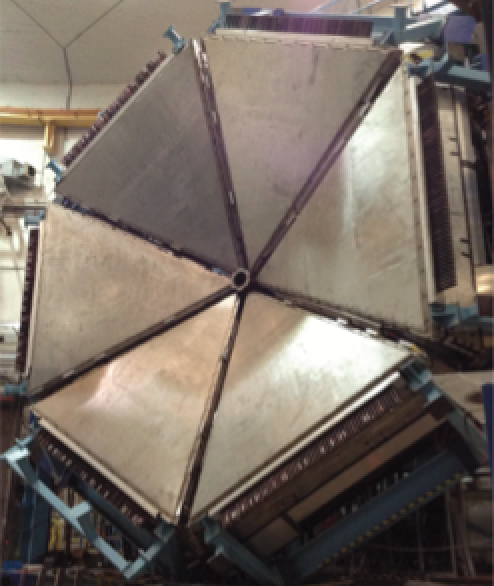
\includegraphics[width=0.60\textwidth,natwidth=610,natheight=642]{PCAL.png}}}
\end{picture} 
\caption{PCAL after installation on the Forward Carriage.}
\label{ec-pcal}
\end{figure}

\subsection{Electromagnetic Calorimeters (EC)}

The CLAS12 detector package uses the existing electromagnetic calorimeter of the CLAS detector~\cite{Amarian:2001zs}
and a new pre-shower calorimeter (PCAL) installed in front of it. Calorimeters in CLAS12 are used primarily for the
identification and kinematical reconstruction of electrons, photons (e.g. from $\pi^\circ \to \gamma \gamma$ and
$\eta \to \gamma  \gamma$ decays ), as well as the detection of neutrons. For details of the construction and the
performance of the PCAL calorimeter (see Ref.~\cite{PCAL}). 

The PCAL and EC are both sampling calorimeters consisting of six modules. The EC consists of EC-inner and EC-outer 
parts, which are separately read out. Each module has a triangular shape with 54 (15/15/24, PCAL/EC-inner/EC-outer) 
layers of 1-cm thick scintillators segmented into 4.5/10-cm (PCAL/EC) wide strips sandwiched between 2.2~mm thick lead
sheets. The total thickness corresponds to approximately 20.5 radiation lengths. Scintillator layers are grouped into three
readout views with 5/5/8, PCAL/EC-inner/EC-outer, layers per view, providing several cm resolution of energy clusters. The
light from each scintillator readout group is routed to the photomultiplier tubes via flexible optical fibers.  Fig.~\ref{ec-pcal}
shows the PCAL during assembly and its response to cosmic ray events after installation in CLAS12.

\begin{figure}[htbp]
\vspace{5.8cm}
\begin{picture}(50,50)
\put(30,-5)
{\hbox{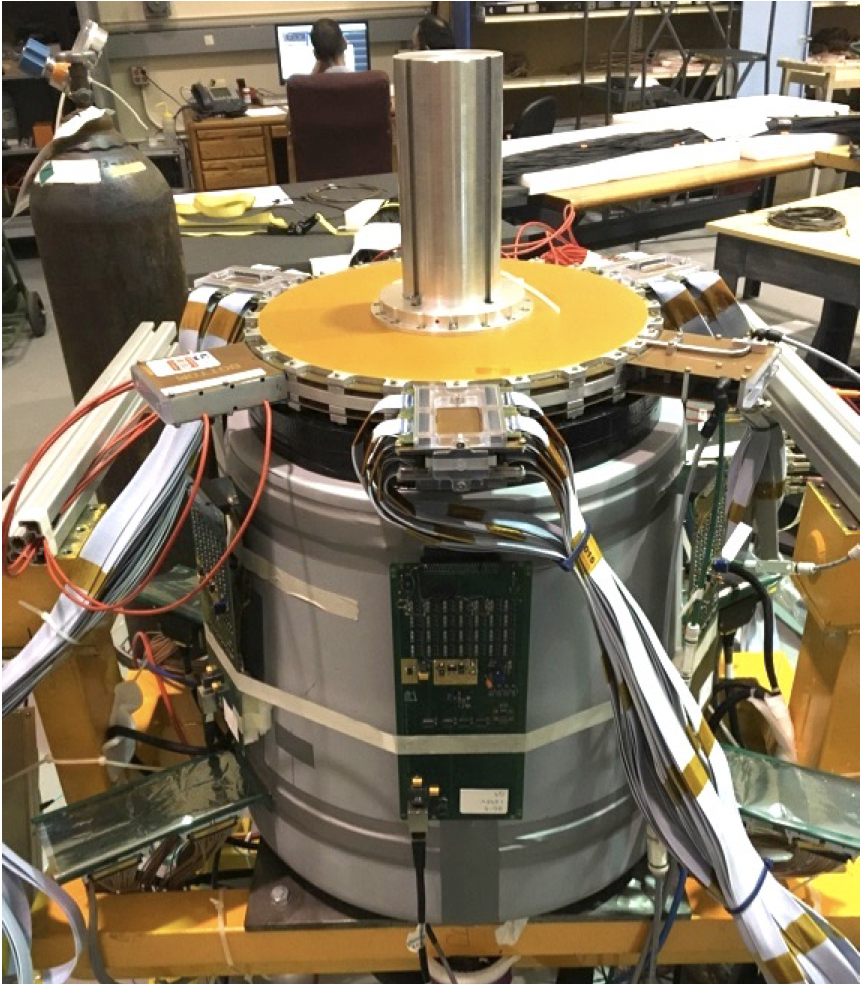
\includegraphics[width=0.48\textwidth,natwidth=610,natheight=642]{FT-photo.png}}}
\end{picture} 
\caption{The Forward Tagger arrangement during cosmic ray testing, before installation in CLAS12. The lower part
  shows the electromagnetic calorimeter composed of lead-tungstate crystals. The top part shows the tracking disks.  }
\label{ft-photo}
\end{figure}

\begin{figure*}[htbp]
\vspace{4.7cm}
\begin{picture}(50,50)
\put(60,0)
{\hbox{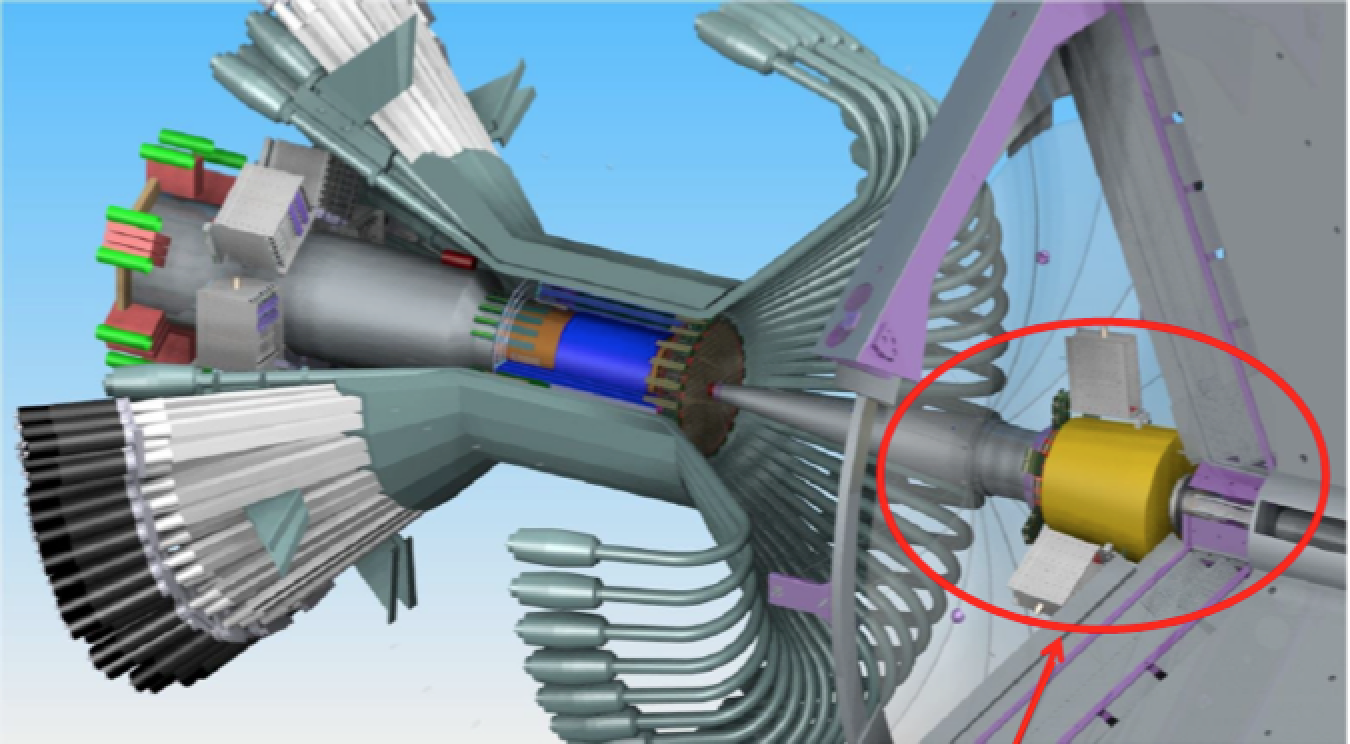
\includegraphics[width=0.45\textwidth,natwidth=610,natheight=642]{CD-FT.png}}}
\end{picture} 
\caption{The Forward Tagger arrangement downstream of Central Detector in front of the Torus magnet warm bore
  entrance.}
\label{ft}
\end{figure*}

\subsection{Forward Tagger (FT)}

Particles scattered at polar angles from $2.5^\circ \le \theta \le 4.5^\circ $ are detected in the calorimeter and the
micro-strip gas tracker and hodoscope of the Forward Tagger (FT). The FT extends the CLAS12 capabilities to detect
electrons and photons at very forward polar angles. The detection of forward-going scattered electrons enables the
execution of electroproduction experiments at very low photon virtuality $Q^2$ providing an energy-tagged, linearly
polarized, high-intensity, quasi-real photon beam. This configuration enables execution of an extensive hadron spectroscopy
program. The FT is comprised of an electromagnetic calorimeter with 332 lead-tungstate (PbWO$_4$) crystals to identify
electrons,  measure the electromagnetic shower energy, and provide a fast trigger signal. The tracking system in front of
the calorimeter  measures the scattering angles, and a scintillator hodoscope aids in separating electrons and high-energy
photons. Fig.~\ref{ft-photo} shows a photograph of the FT during cosmic ray studies before its installation in CLAS12.
Further details are described in ~\cite{FT}. Fig.~\ref{ft} shows a rendering of the FT setup near the entrance to the
warm bore of the Torus magnet.   

\section{CLAS12 Central Detector (CD)} 

Particles scattered from the target at polar angles in the range from $35^\circ$  to $120^\circ$ are detected in the Central
Detector with its own particle identification and tracking detectors. Charged particles are detected in the Central
Time-of-Flight (CTOF) detector with full $360^\circ$ coverage in azimuthal angle, and tracked in the Central Vertex
Tracker (CVT). Neutron detection is provided by the Central Neutron Detector (CND) located radially outside of the CVT
and the CTOF.  Fig.~\ref{CVT} shows the full assembled CVT before installation in the solenoid magnet. The fully assembled
CD is displayed in  Fig.~\ref{CDinSol} after installation in the Solenoid.  Fig.~\ref{CDback} shows the installed Central
Detector from the back end.    

\begin{figure}[htbp]
\vspace{4.0cm}
\begin{picture}(50,50)
\put(0,0)
{\hbox{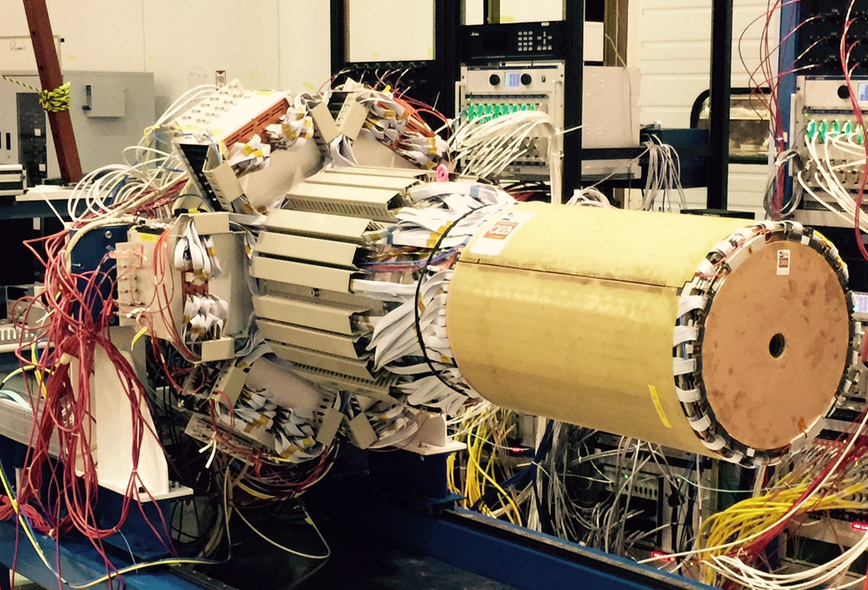
\includegraphics[width=0.45\textwidth,natwidth=610,natheight=642]{CVT.png}}}
\end{picture} 
\caption{Central Vertex Tracker, fully assembled with the SVT, BMT, and FMT. The BMT and FMT are shown on the
  outside. The SVT is encapsulated and hidden from view. }
\label{CVT}
\end{figure}

\begin{figure}[htbp]
\vspace{5.0cm}
\begin{picture}(50,50)
\put(15,-10)
{\hbox{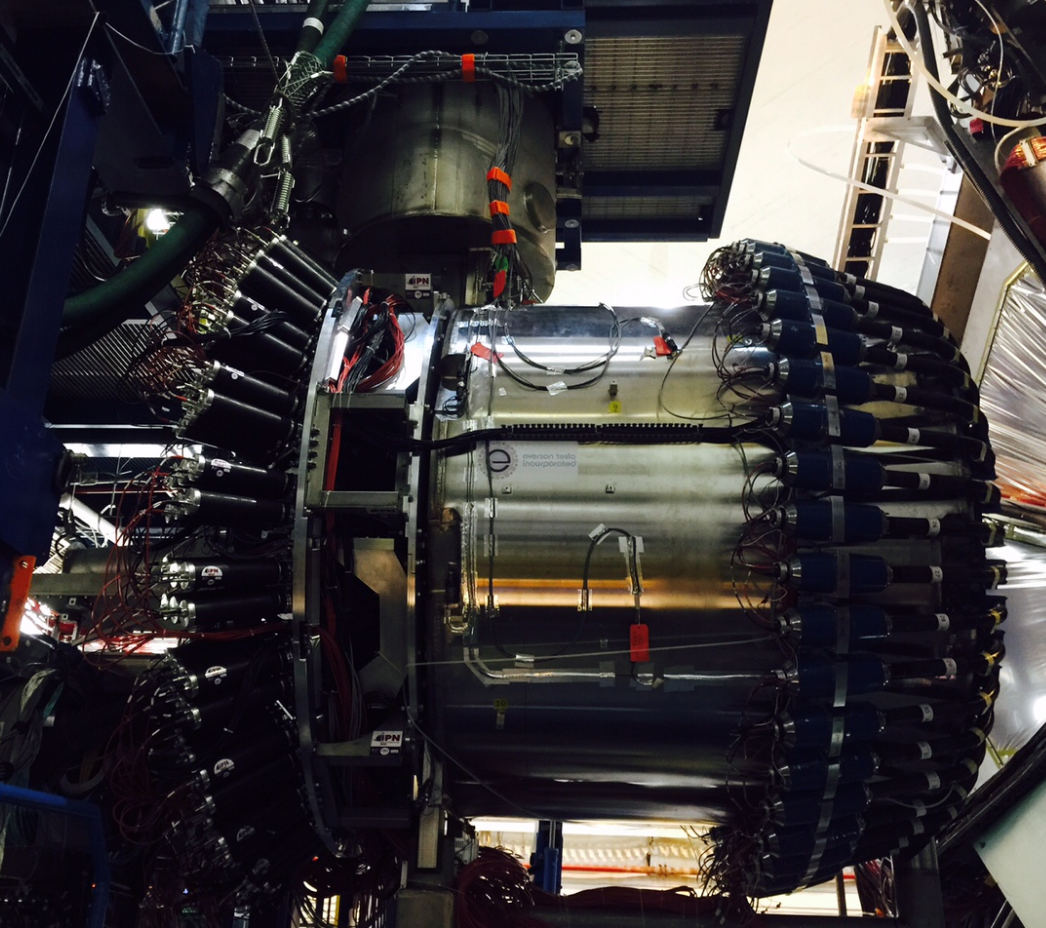
\includegraphics[width=0.35\textwidth,natwidth=610,natheight=642]{CLAS12-CD-front.png}}}
\end{picture} 
\caption{The Central Detector installed in the Solenoid magnet in a side view. The readout photomultiplier tubes are seen
  at the upstream end (left) and at the downstream end (right) of the Solenoid. }
\label{CDinSol}
\end{figure}

\begin{figure}[htbp]
\vspace{4.2cm}
\begin{picture}(50,50)
\put(3,0)
{\hbox{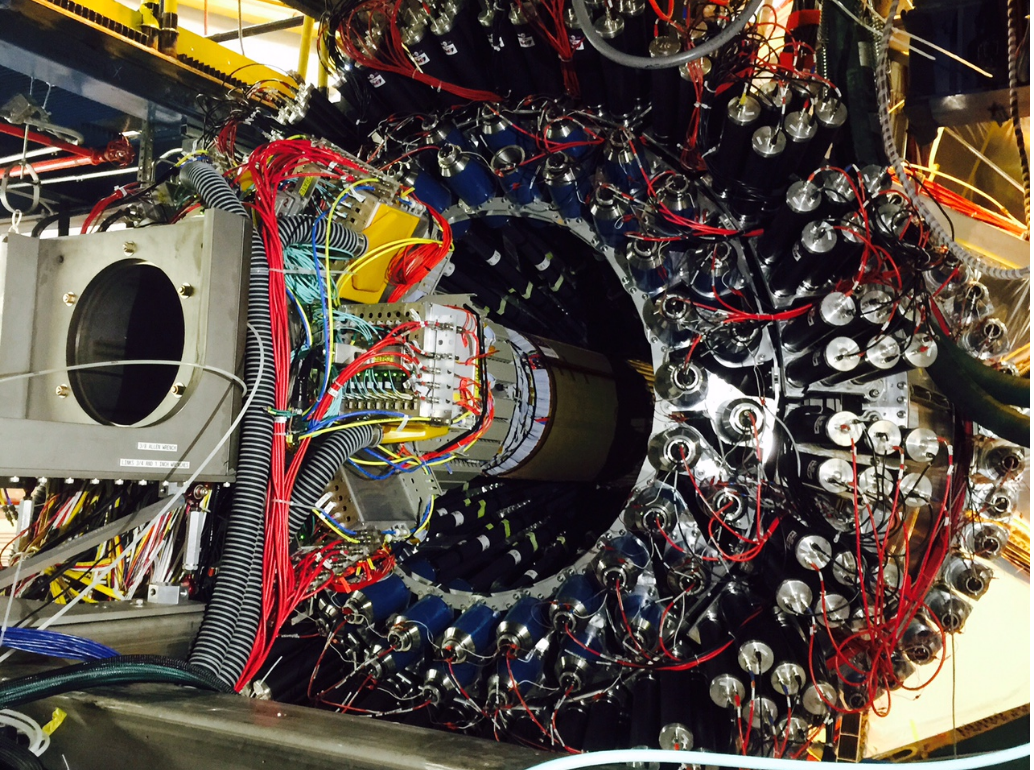
\includegraphics[width=0.38\textwidth,natwidth=610,natheight=642]{CLAS12-CD.png}}}
\end{picture} 
\caption{The Central Detector seen from the back end. The CVT is shown at the left end in retracted position for
  maintenance. During operation the CVT is  fully inserted into the warm bore of the magnet. }
\label{CDback}
\end{figure}

\subsection{Central Vertex Tracker (CVT)}

The CLAS12 CVT is a part of the Central Detector and is used to measure the momentum and determine the vertex of charged
particles scattered from the production target, which is centered within the Solenoid magnet. It contains two separate trackers,
a Silicon Vertex Tracker (SVT) and a Barrel Micromesh Tracker  (BMT). The SVT system includes 3 regions with 10, 14, and 18
sectors of double-sided modules of silicon sensors instrumented with digital readout ASICs and FSSR2s. The readout pitch is
156~$\mu$m, and the total number of channels is 33,792. The BMT contains 3 layers of strips along the beamline and 3 layers
of circular readout strips around the beamline, with a total number of 15,000 readout elements. The BMT provides important
improvements in momentum resolution, and in tracking efficiency. Each layer is arranged azimuthally in 3 sectors of 125$^\circ$
azimuthal coverage. The system operates at full design luminosity of $10^{35}\rm~{cm^{-2}s^{-1}}$. Another component is the
Forward Micromegas Tracker (FMT), consisting of 6 layers with 6,000 readout elements. It  is integrated mechanically with the
CVT to provide a compact tracking system, but covers the polar angle range from 5$^\circ$ to $35^\circ$ and provides improved
vertex reconstruction for forward scattered charged particles.

\subsection{Central Time-of-Flight (CTOF)}

The CTOF system is used for the identification of charged particle emerging from the target via time-of-flight measurements.
The CTOF includes 48 plastic scintillators with double-sided photomultiplier readout via, respectively, 1.0~m-long upstream and
1.6~m-long downstream focusing light guides. The array of 48 counters forms a hermetic barrel around the target and the CVT.
The barrel is aligned with the beam axis inside the 5~T Solenoid magnet. The photomultipliers are placed in a region of 0.1~T
fringe field of the Solenoid and enclosed within a triple layer dynamical magnetic shield~\cite{Baturin:2012zz} that provides
less than 0.2~G internal field near the PMT photocathode. The CTOF system is designed to provide time resolution of 75~ps
for charged particle identification in the CLAS12 Central Detector. Details are described in Ref.~\cite{CTOF}.  

\subsection{Central Neutron Detector (CND)}

The CLAS12 CD is also equipped with the CND that follows the CTOF radially and allows the detection of neutrons in the
momentum range of 0.2~GeV to 1.0~GeV by measurement of their time-of-flight from the target to the hit position and
the energy deposition in the scintillator layers. The detector is made of three layers of scintillator paddles (48 paddles per
layer), coupled two-by-two at the downstream end with semi-circular light guides and read out at the back end by
photomultipliers placed outside of the high magnetic field region. The scintillators are connected to 1.5-m-long bent light
guides. The CND is the last radial detector within the warm bore of the Solenoid magnet cryostat. Fig.~\ref{ctof-cnd} (right)
displays the upstream readout end of the CND. 

\begin{figure*}[ht]
\vspace{3.7cm}
\begin{picture}(50,50)
\put(25,0)
{\hbox{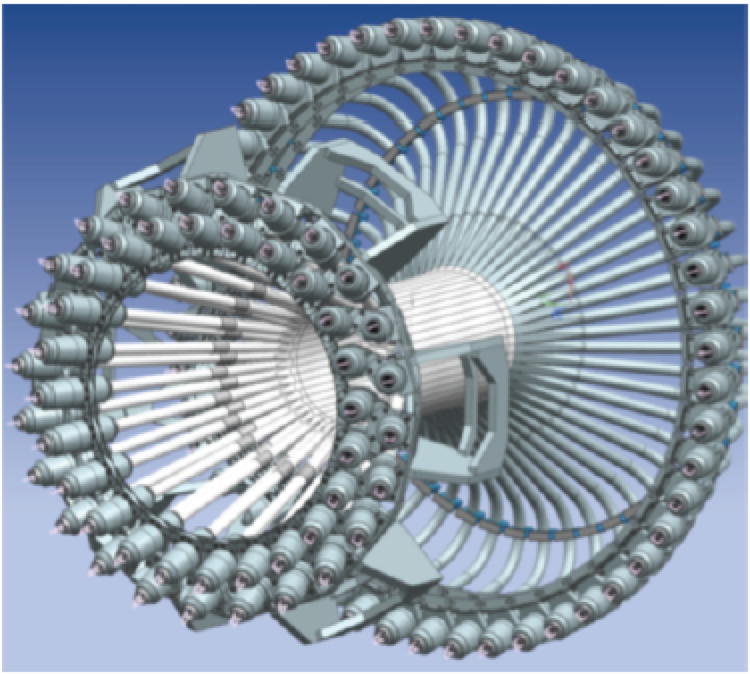
\includegraphics[width=0.45\textwidth,natwidth=610,natheight=642]{CTOF-pic.png}}}
\put (225,0)
{\hbox{\includegraphics[width=0.43\textwidth,natwidth=610,natheight=642]{cnd-ctof.png}}}
\end{picture} 
\caption{Left: The Central Time-of-Flight detector with the 48 scintillator bars, and the 48 photomultipliers on each end
  of the scintillators. Right: The fully assembled CD as seen from its upstream end with the 144 CND light guides and
  photomultipliers at the three outermost rings, and the 48 PMTs of the CTOF (two inner rings). {\bf GET ENGINEERING
 DRAWINGS FOR LEFT PANEL.}} 
\label{ctof-cnd}
\end{figure*} 

\section{CLAS12 Offline Software}  

The CLAS12 offline software system is designed to analyze large amounts of beam-induced experimental data acquired
during production and cosmic ray runs for alignment and calibration purposes. The system is a Service Oriented software
Architecture, which consists of three major components, the event reconstruction, visualization, and calibration monitoring
services, as well as detector and event simulations.  

During the CLAS12 design phase a realistic simulation package based on Geant4 was developed to aid in the optimization 
of the detector hardware response to beam interactions in terms of resolution, robustness of operation at high luminosities,
details of the beamline design, and other aspects. Details are described in Ref.~\cite{Software}. 

\subsection{Monte Carlo Simulations}

A critical part of operating an open large-acceptance detector system at high luminosities is the simulation not only of hadronic
events but also, and more importantly, the simulation of the beam-related accidental hits in the tracking system. The sources
of accidentals are primarily the beam electron elastically scattered off atomic electrons (M{\"o}ller electrons) and their
secondary interaction with beamline components. The production rate is orders of magnitude larger than the hadronic production
rate. These background sources have to be shielded through careful design of magnetic channeling and a proper design of the
beamline shielding and the vacuum pipe to minimize interaction of these electrons with high-$Z$ material. The availability of a
realistic simulation package was essential for optimal design of the CLAS12 integrated detector concept. The strong solenoid
field is essential in channeling the scattered M{\"o}ller electrons through the beam enclosure to avoid interactions with the 
beamline materials. Fig.~\ref{gemc-event}  shows a single electron track event at 1/30 of the full luminosity in a time window
of 250~ns, corresponding to the minimal time  window in the R1 drift chambers. 
 
A realistic simulation package is essential for the normalization of cross sections, especially to take into account the 
detector occupancies for data taking at luminosities near or above the maximum design luminosity where the track 
reconstruction efficiency can be significantly affected by accidentals. In order to quantitatively account for this, data
were taken at different beam current, i.e. different luminosities with randomly triggered events. Data from these randomly
triggered events were merged with simulated physics events to study the loss of real tracks for different data runs. For
details on the simulation effort for CLAS12, see Ref.~\cite{GEMC}.    

\begin{figure*}[ht]
\vspace{10.0cm}
\begin{picture}(50,50)
\put (35,180)
{\hbox{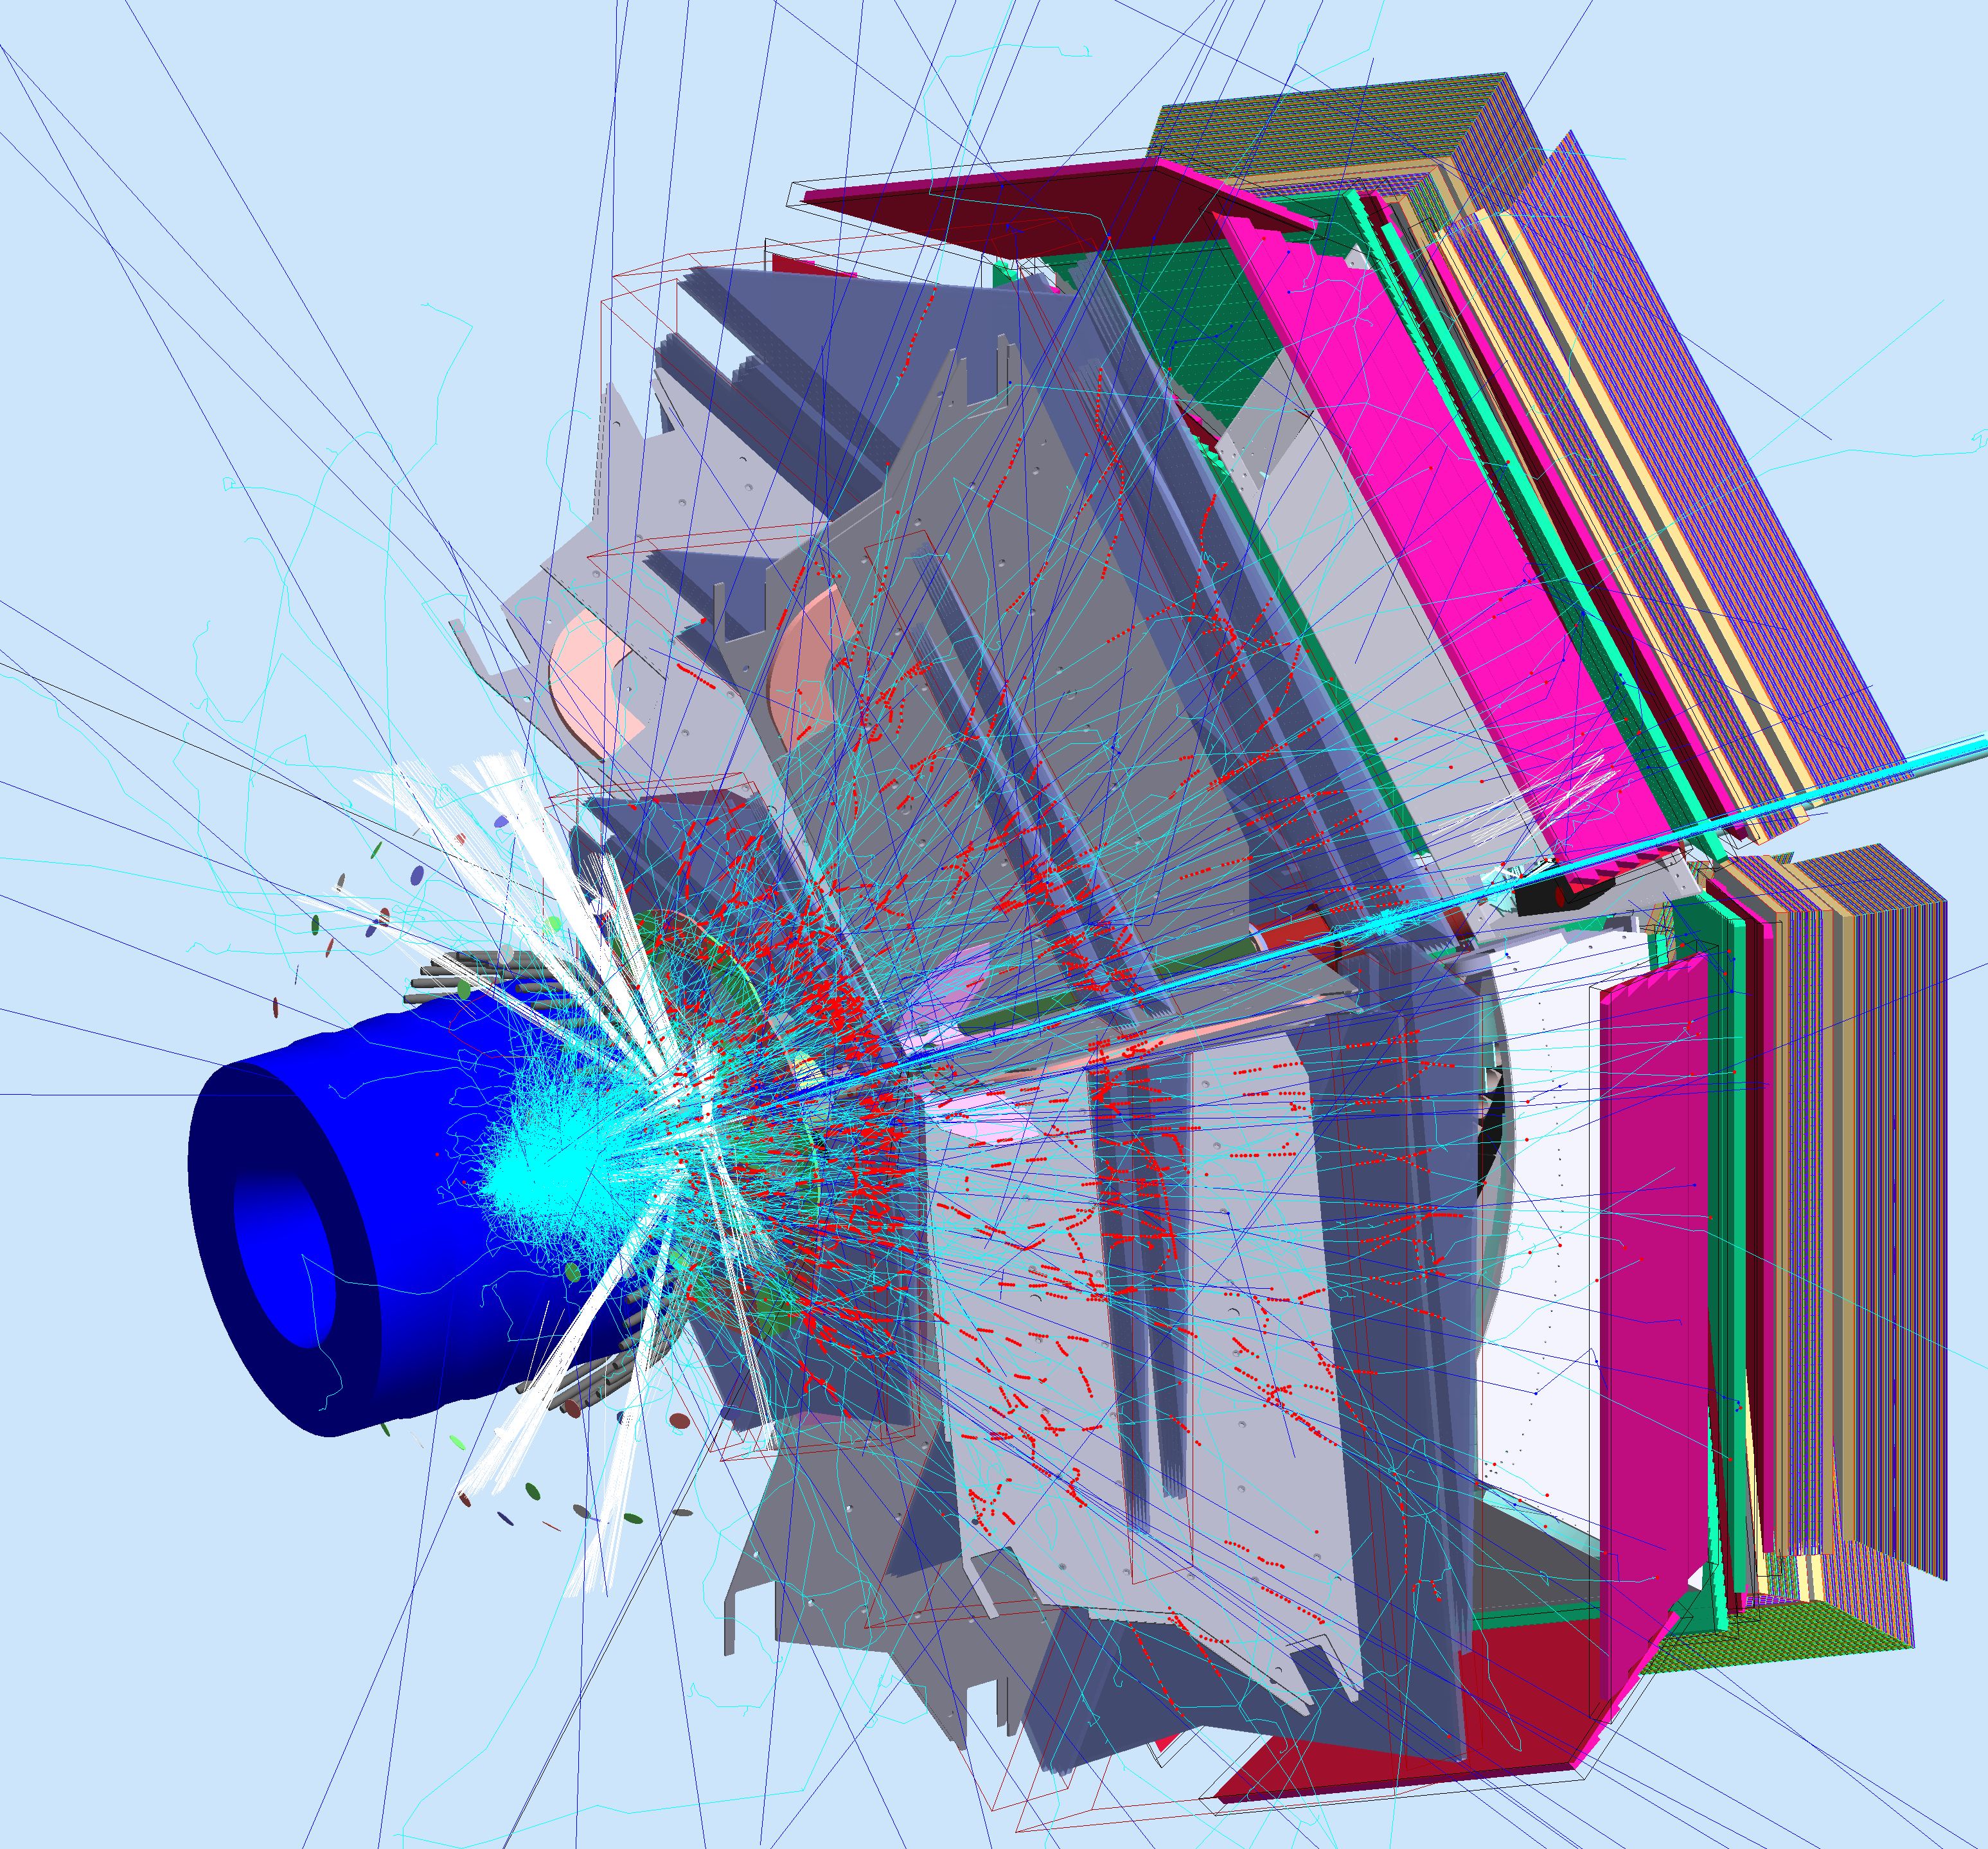
\includegraphics[width=0.104\textwidth,natwidth=610,natheight=642]{50percentNoSolenoidNoTorus1.png}}}
\put (240,180)
{\hbox{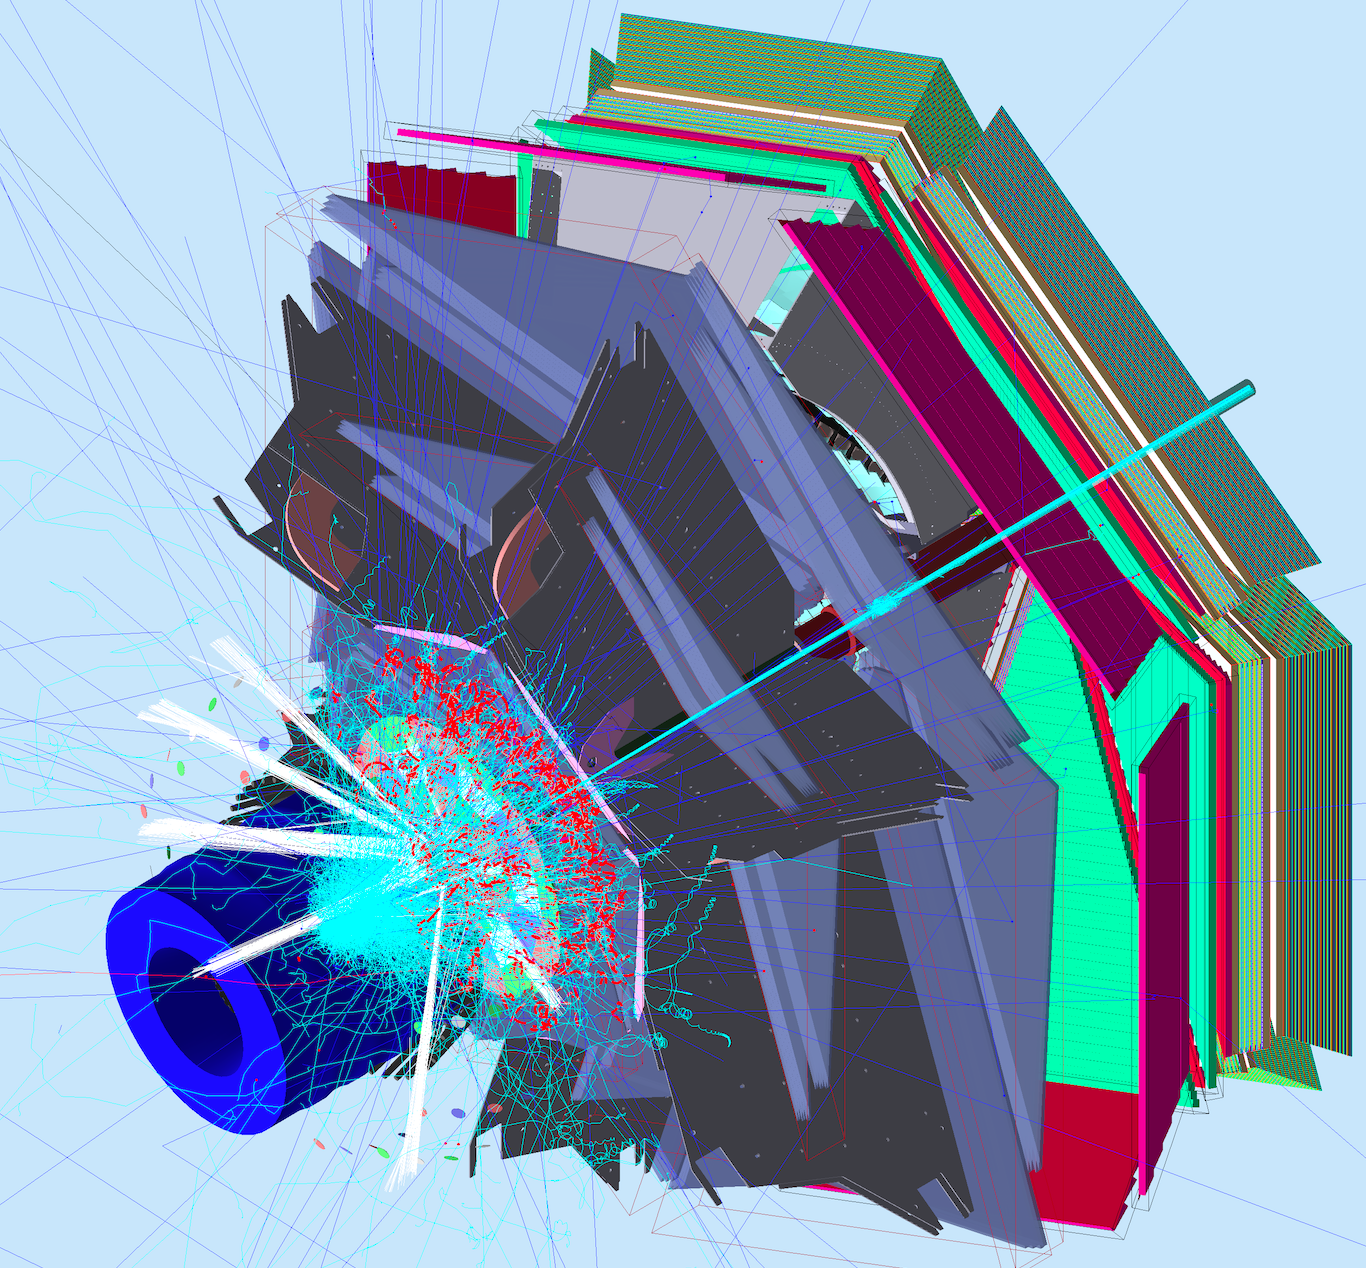
\includegraphics[width=0.24\textwidth,natwidth=610,natheight=642]{50percentNoSolenoid2a.png}}}
\vspace{0.3cm}
\put (35,-5)
{\hbox{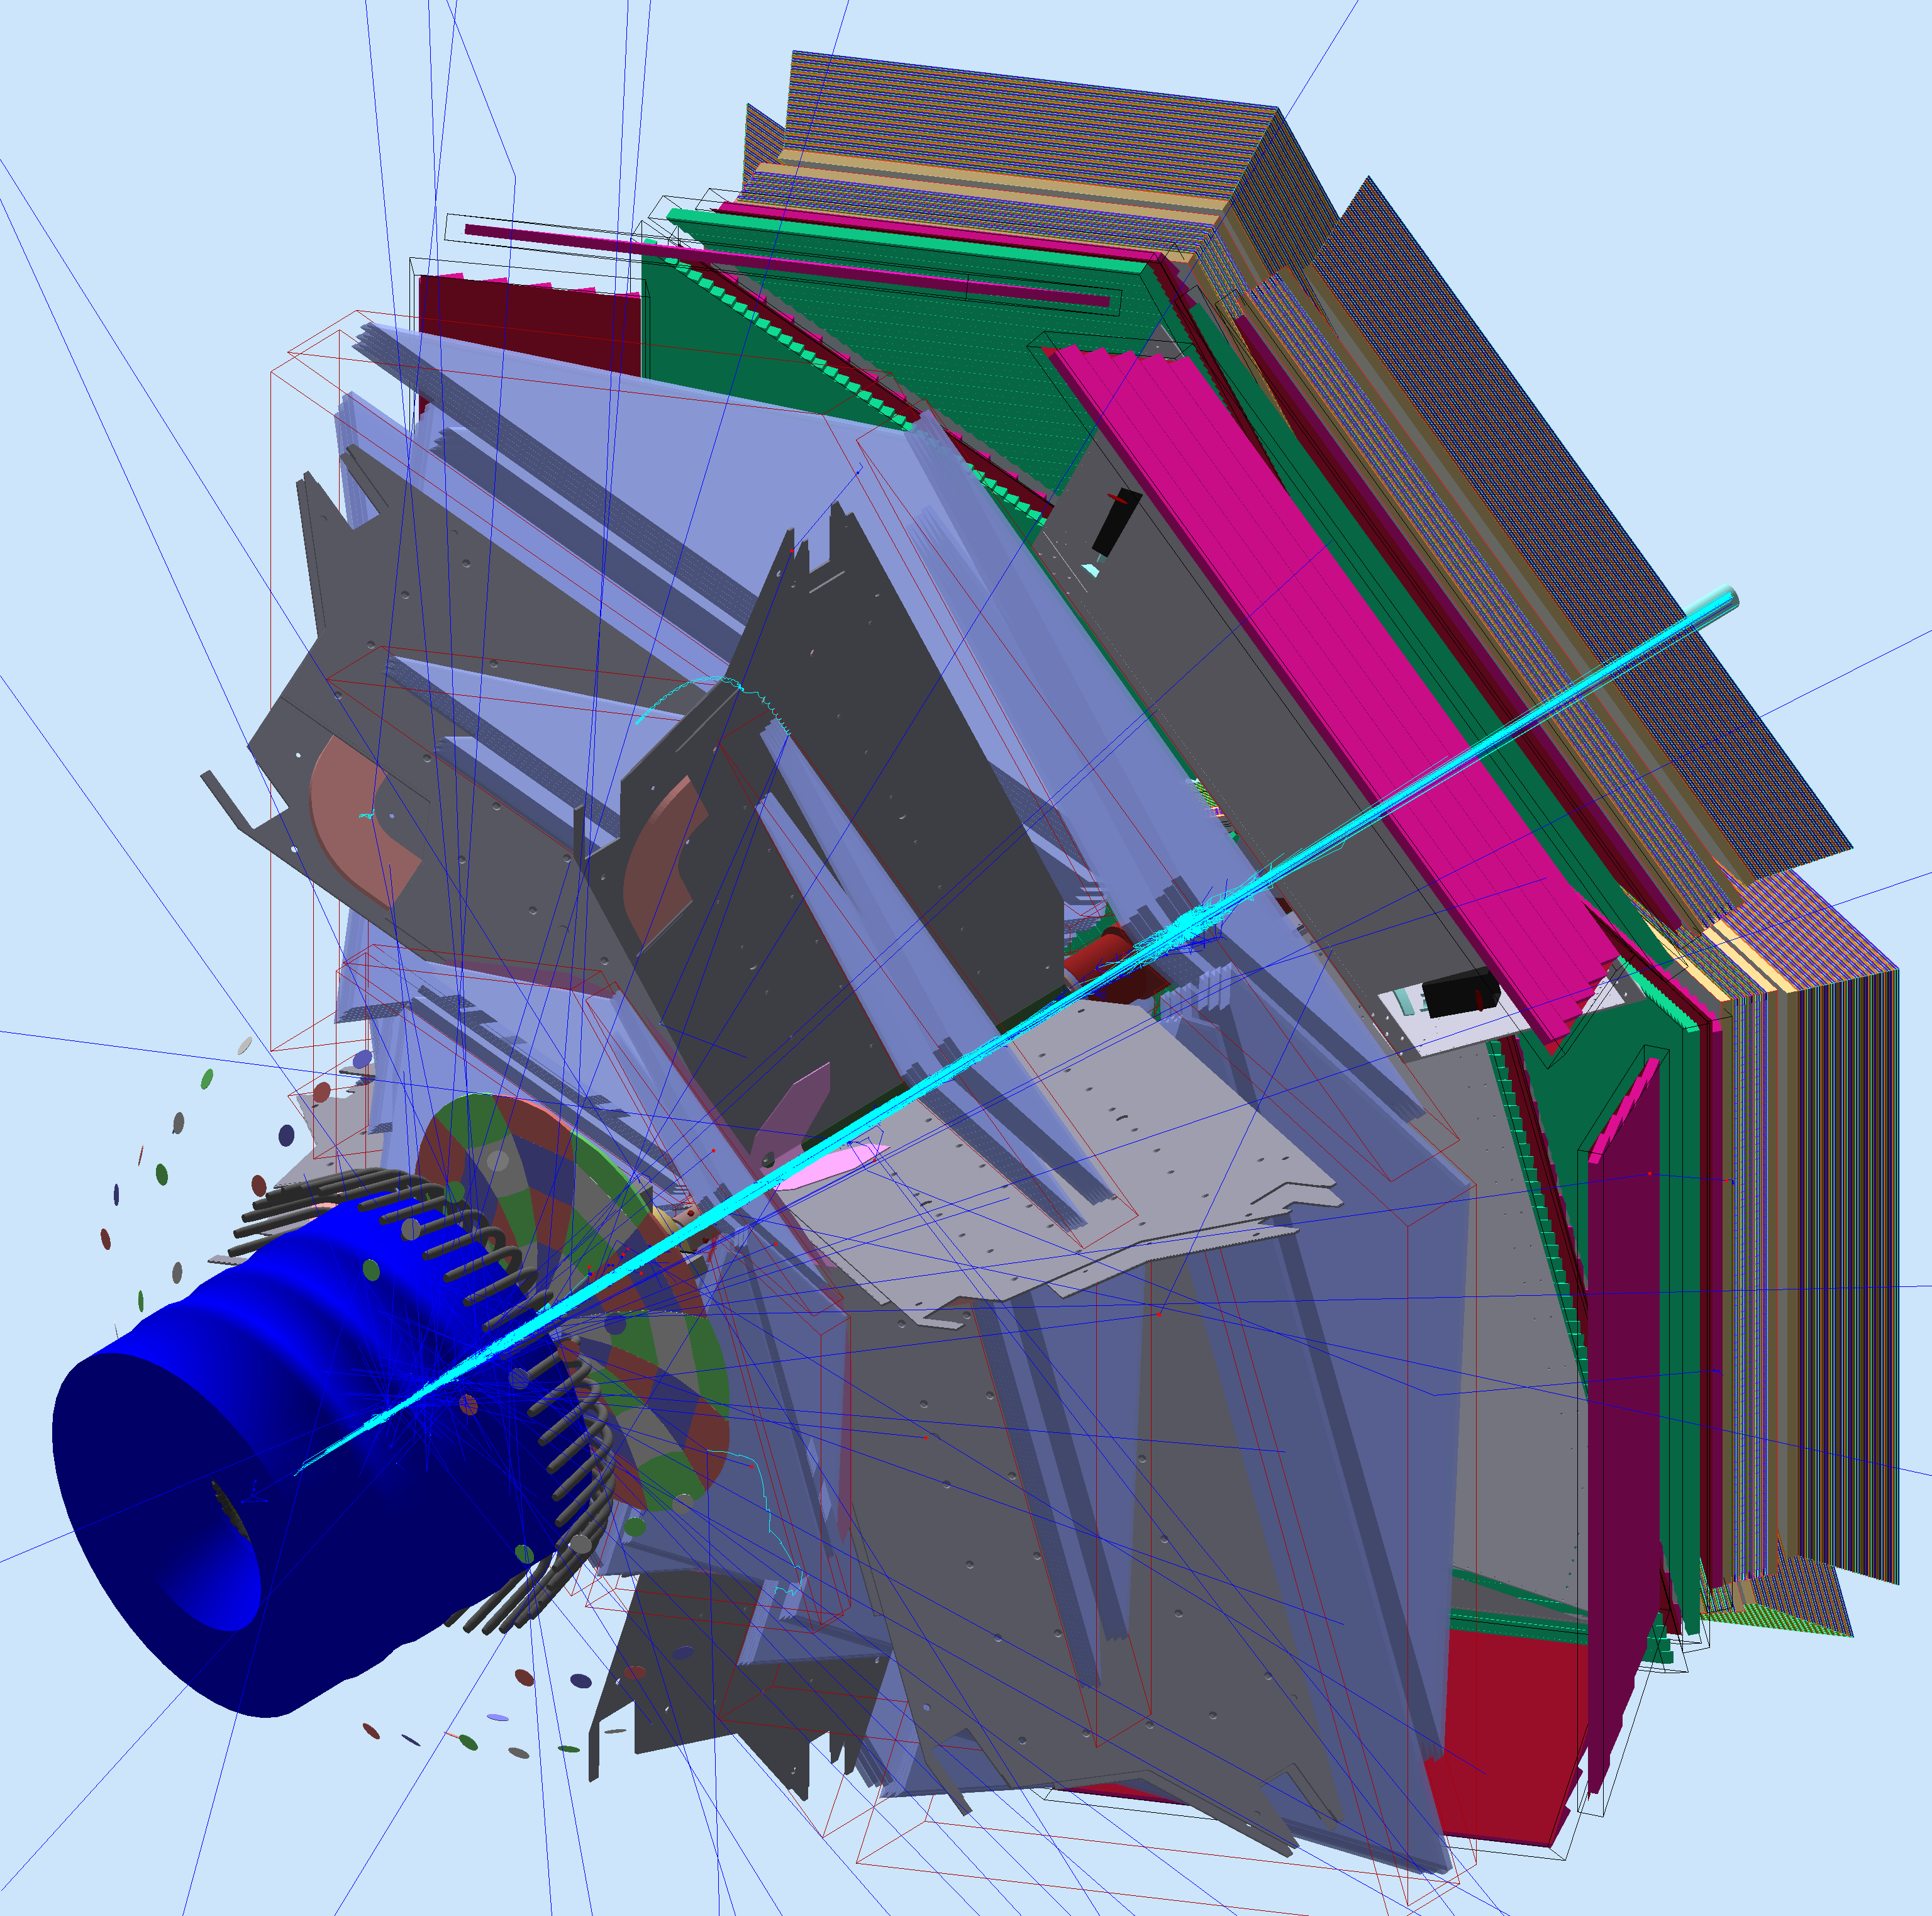
\includegraphics[width=0.104\textwidth,natwidth=610,natheight=642]{100percentSolenoid.png}}}
\put (240,-5)
{\hbox{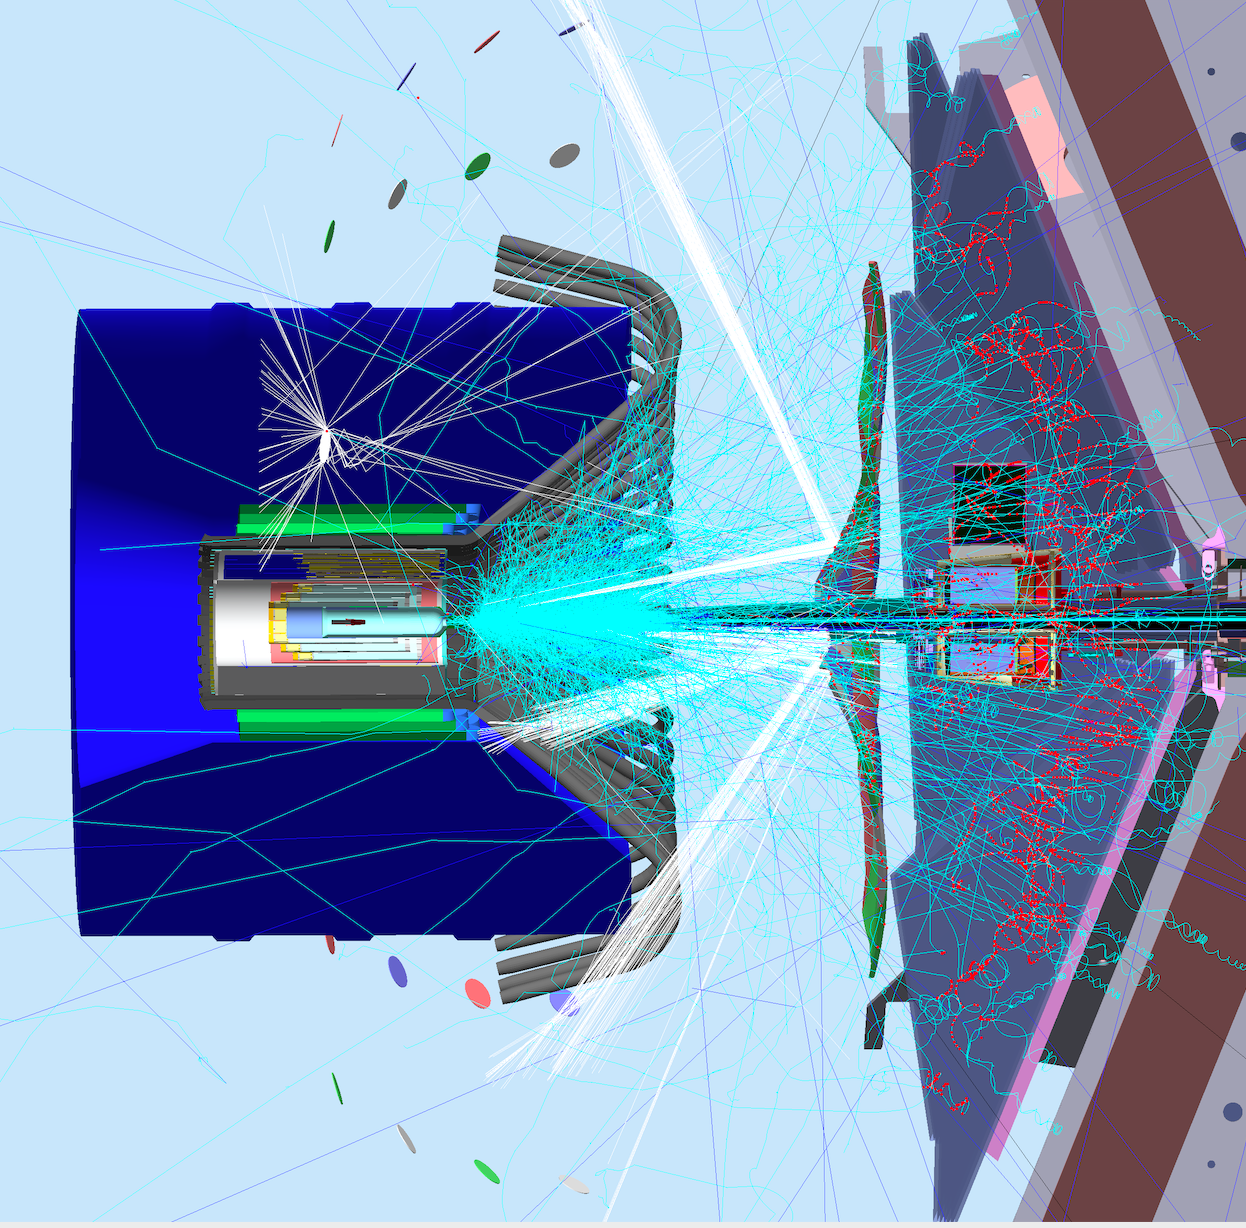
\includegraphics[width=0.256\textwidth,natwidth=610,natheight=642]{50percentNoSolenoidCut3a.png}}}
\end{picture} 
\caption{Geant4 representations of accidental background events occurring within a 250~ns time window at different
  magnetic field configurations and 50\% of design luminosity. Top left: Solenoid field is OFF and Torus field is OFF. Top
  right: Solenoid field is OFF and Torus field is ON. Bottom: right Close-up of Top: right.  Bottom left: Solenoid field is
  ON and Torus field is ON at 100\% design luminosity. Color code: cyan: primary electrons, red: energy loss in detectors,
  blue: photons, white: Cherenkov light.} 
\label{gemc-event}
\end{figure*}

\subsection{Event Reconstruction} 

Event reconstruction in the CLAS12 FD consists of the identification of charged and neutral particles along with the 
computation of their 3-momenta. Charged-particle reconstruction requires both particle tracking and particle 
time-of-flight (TOF) information. 

\begin{figure}[htbp]
\vspace{7.0cm}
\begin{picture}(50,50)
\put(35,200)
{\hbox{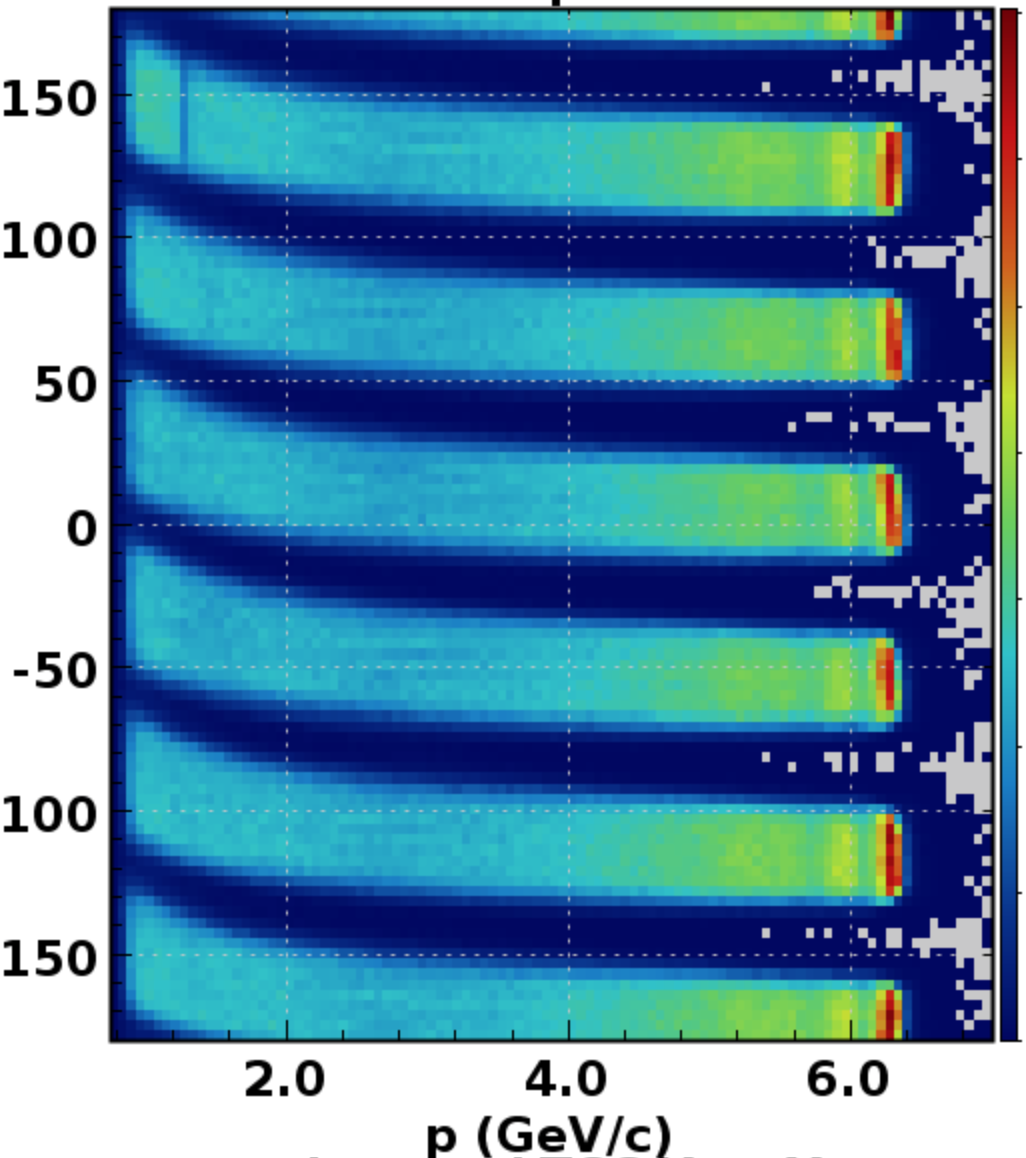
\includegraphics[width=0.30\textwidth,natwidth=610,natheight=642]{neg-tracks.png}}}
\put(25,-5)
{\hbox{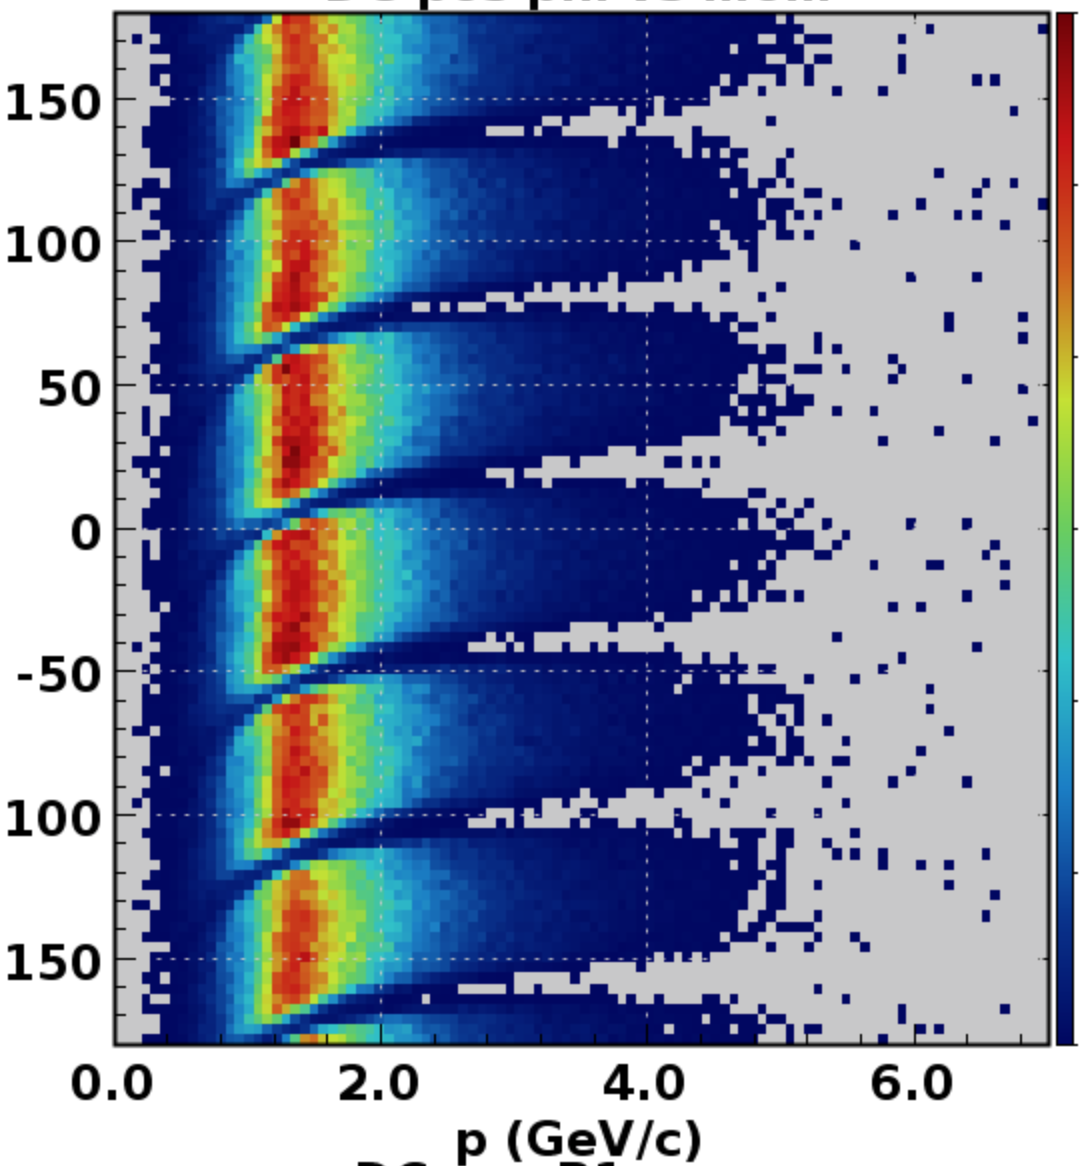
\includegraphics[width=0.30\textwidth,natwidth=610,natheight=642]{pos-tracks.png}}}
\end{picture} 
\caption{Azimuthal angle acceptances versus momentum in the CLAS12 FD. Top: negative tracks including electrons.
  Bottom: positive tracks. The curving at low momentum is a reflection of the azimuthal motion due to the Solenoid
  magnetic field. Data were taken at 6.5~GeV electron beam energy. {\bf may replace with the same for in-sector
  coordinate system for straight distributions.}} 
\label{neg-pos}
\end{figure}

Track reconstruction in the FD begins with hits in the drift chamber cells that can be connected to define a hit-based
track, when at least 4 out of 6 layers in each superlayer have hits, and in at least 5 out of 6 superlayers. The timing
information is used to determine a time-based track and the particle momentum and flight path, while the TOF gives the
particle velocity ($\beta$) when combined with flight-path information. The momentum and velocity information are
combined to give the particle mass: $m = p/\beta\gamma$. Electron identification additionally requires the track to
match in time and position with both an HTCC hit and an isolated shower in the ECAL. The energy of the shower must be
consistent with the track momentum from the drift chambers.  

Charged particles are tracked in each sector separately using the 3 regions of drift chambers in each sector. Most
tracks are confined within one sector as the magnet optics and the massive mechanical support of the Torus coils
prevent most tracks from crossing from one sector into a neighboring sector. In rare cases low momentum charged
pions can cross from one sector into the opposite sector traversing through the beam pipe . Such tracks are not
reconstructed but they are included in the event simulation. Distributions of charged particles in azimuthal angle
versus momentum are shown in Fig.~\ref{neg-pos}.  Fig.~\ref{vertex} shows the production vertex as reconstructed
in the FD tracking system (w/o the FMT). 

Neutral particles are detected in either the calorimeters or in the scintillator material of FTOF (or both). The 
reconstruction begins by finding isolated clusters of energy, and determining the spatial location, deposited 
energy, and the time of the cluster. Neutral particle candidates are identified as clusters in the outer detectors 
(FTOF, PCAL, EC) that do not match any charged particle track. For high-energy photons that deposit all of their 
energy in the calorimeters, the energy is calculated from the signal pulse height in the calorimeters. The momenta 
of neutrons are computed from their flight time as determined by the time signal in the calorimeters and, 
when relevant, the matched FTOF counter. In either case, the angle of the neutral particle trajectory is determined
from the position of the cluster at the face of the calorimeters ({\bf IS THIS STILL CORRECT?????}).  

\begin{figure}[htbp]
\vspace{5.0cm}
\begin{picture}(50,50)
\put(3,-5)
{\hbox{\includegraphics[width=0.40\textwidth,natwidth=610,natheight=642]{tracking_vertices.png}}}
\end{picture} 
\caption{Vertex reconstruction in FD. The upper row shows the reconstructed vertices in the production frame along
  the beamline for negative tracks (left) and positive tracks (right). The Solenoid field causes the vertices to be shifted
  in opposite directions from the center depending on their respective charges. The bottom row shows the projected
  vertices within the sector frame. They exhibit a track occupancy that is symmetric inside their respective sectors. The
  sector boundaries are clearly visible.} 
\label{vertex}
\end{figure}

\begin{figure*}[htbp!]
\vspace{6.0cm}
\begin{picture}(50,50)
\put(10,0)
{\hbox{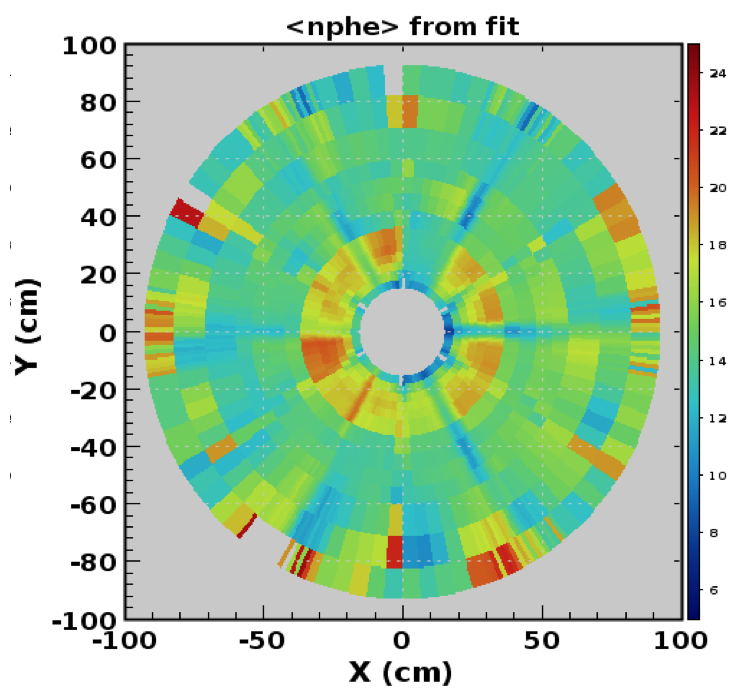
\includegraphics[width=0.55\textwidth,natwidth=610,natheight=642]{htcc-pel.png}}}
\put(240,0)
{\hbox{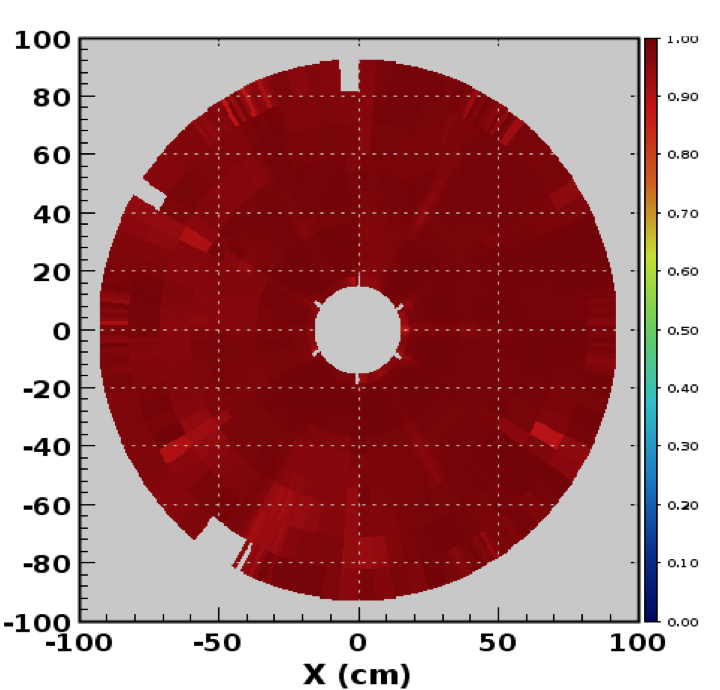
\includegraphics[width=0.55\textwidth,natwidth=610,natheight=642]{htcc-eff.png}}}
\end{picture}
\caption{ Left: Distribution of the average number of photoelectrons in the HTCC in polar and azimuthal angles. The average
  number of photoelectrons ranges from 10 at the interfaces of mirror facets, to 15  in the other areas. Right: Distribution of
  HTCC efficiencies in polar and in azimuthal angles. The electron detection efficiency is over 95\% in the full phase space
  covered by the HTCC. {\bf GET RIGHT FIGURE WITH HIGH EFFICIENCY IN LIGHT COLORS.}} 
\label{htcc-eff}
\end{figure*}

\begin{figure}[htbp]
\vspace{4.5cm}
\begin{picture}(50,50)
\put(0,0)
{\hbox{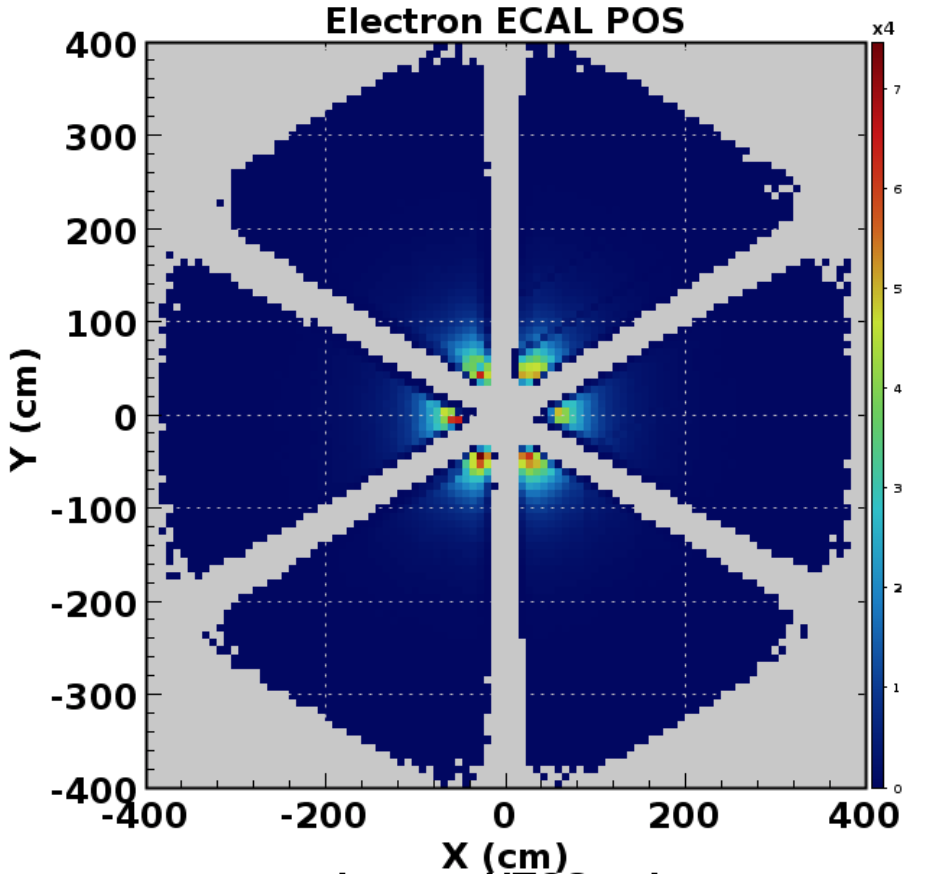
\includegraphics[width=0.40\textwidth,natwidth=610,natheight=642]{electron-xy.png}}}
\end{picture} 
\caption{Distribution of electron track x and y coordinates propagated to the ECAL front face. {\bf MAYBE DO IT
  IN LOG SCALE?}} 
\label{electrons-xy}
\end{figure}

For all events, precise determination of the interaction time or event start time is required. For events where the
scattered electron is detected, the event start time is derived from arrival time of the electron at the FTOF counters,
corrected for flight path and signal delays.  The average time resolution for electrons reconstructed in CLAS12 FD is
80~ps. A more accurate event start time is obtained by replacing the measured electron start time with the 499
(249.5)~MHz accelerator RF signal that determines the beam bunch associated with the event. In this way, the event
start time can be determined to within a few ps, thus eliminating a significant contribution to the time resolution for
charged hadrons. This extends the charged particle identification capabilities of CLAS12 towards higher particle
momentum.

\begin{figure}[htbp]
\vspace{4.7cm}
\begin{picture}(50,50)
\put(10,-10)
{\hbox{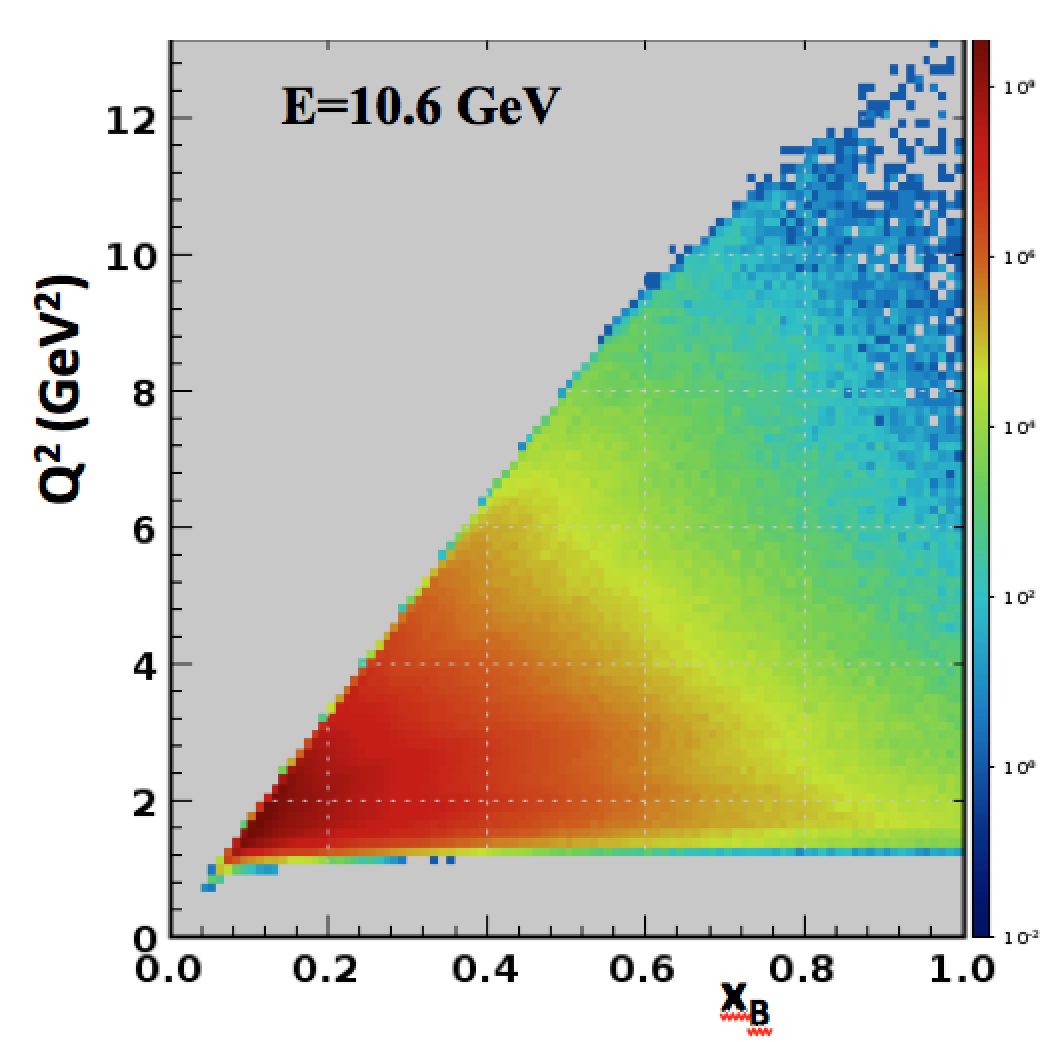
\includegraphics[width=0.35\textwidth,natwidth=610,natheight=642]{e-inclusive.png}}}
\end{picture} 
\caption{Inclusive $ep \to eX$ coverage in $Q^2$ vs $x_B$.  The full kinematics is measured simultaneously. The
  kinematic range is given by the beam energy to the left, the elastic scattering kinematics at $x_B = 1$, and by the
  small angle acceptance at $Q^2 \approx 1.0$~GeV$^2$ limit for electrons bending towards the beamline.} 
\label{electron-acceptance}
\end{figure}

\section{CLAS12 Operational Performance}

This section describes the overall performance of the CLAS12 detection system. Most of the experimental programs
require the clean identification and reconstruction of the scattered electron. Electrons are identified by a combination
of signals in the HTCC and energy deposited in the combined electromagnetic calorimeters PCAL and EC and a negative
charged track in the drift chamber tracking system. Of critical importance is the response of the HTCC that operates
between the CD and the entrance to the drift chamber system. Fig.~\ref{htcc-eff} shows the distribution of the
number of photoelectrons and efficiency in the 48 segments of the HTCC that cover the entire azimuthal angle range.
The coordinates of reconstructed electrons at the front face of the PCAL is shown in Fig.~\ref{electrons-xy}. The
distribution is rather uniform in all six sectors showing that the detector systems and the reconstruction software are
working properly. Elastic scattering  of electrons on protons allows for the establishment of any deviations from the ideal
detector geometry and alignment. The coverage in kinematic quantities $Q^2$ and $x_B$ of the scattered electrons
detected in the FD are shown in Fig.~\ref{electron-acceptance}. $Q^2$ is the virtuality of the photon exchanged from
the electron to the proton target, and $x_B$ is the Bjorken scaling variable.

\subsection{Charged Particle Detection in FD}
 
Charged particles acceptances in momentum and azimuthal angles are shown in Fig.~\ref{neg-pos} in the sector frame for
negative and positive charged particles. The difference in the acceptance is due to two factors, the polarity of the Torus
magnet that bends negative particles away from the beamline and positive particles towards the beamline, and the effects
of the solenoid magnetic field that causes an azimuthal motion for positive and negative particles in opposite directions. 

\begin{figure}[htbp]
\vspace{2.0cm}
\begin{picture}(50,50)
\put (-5,-10)
{\hbox{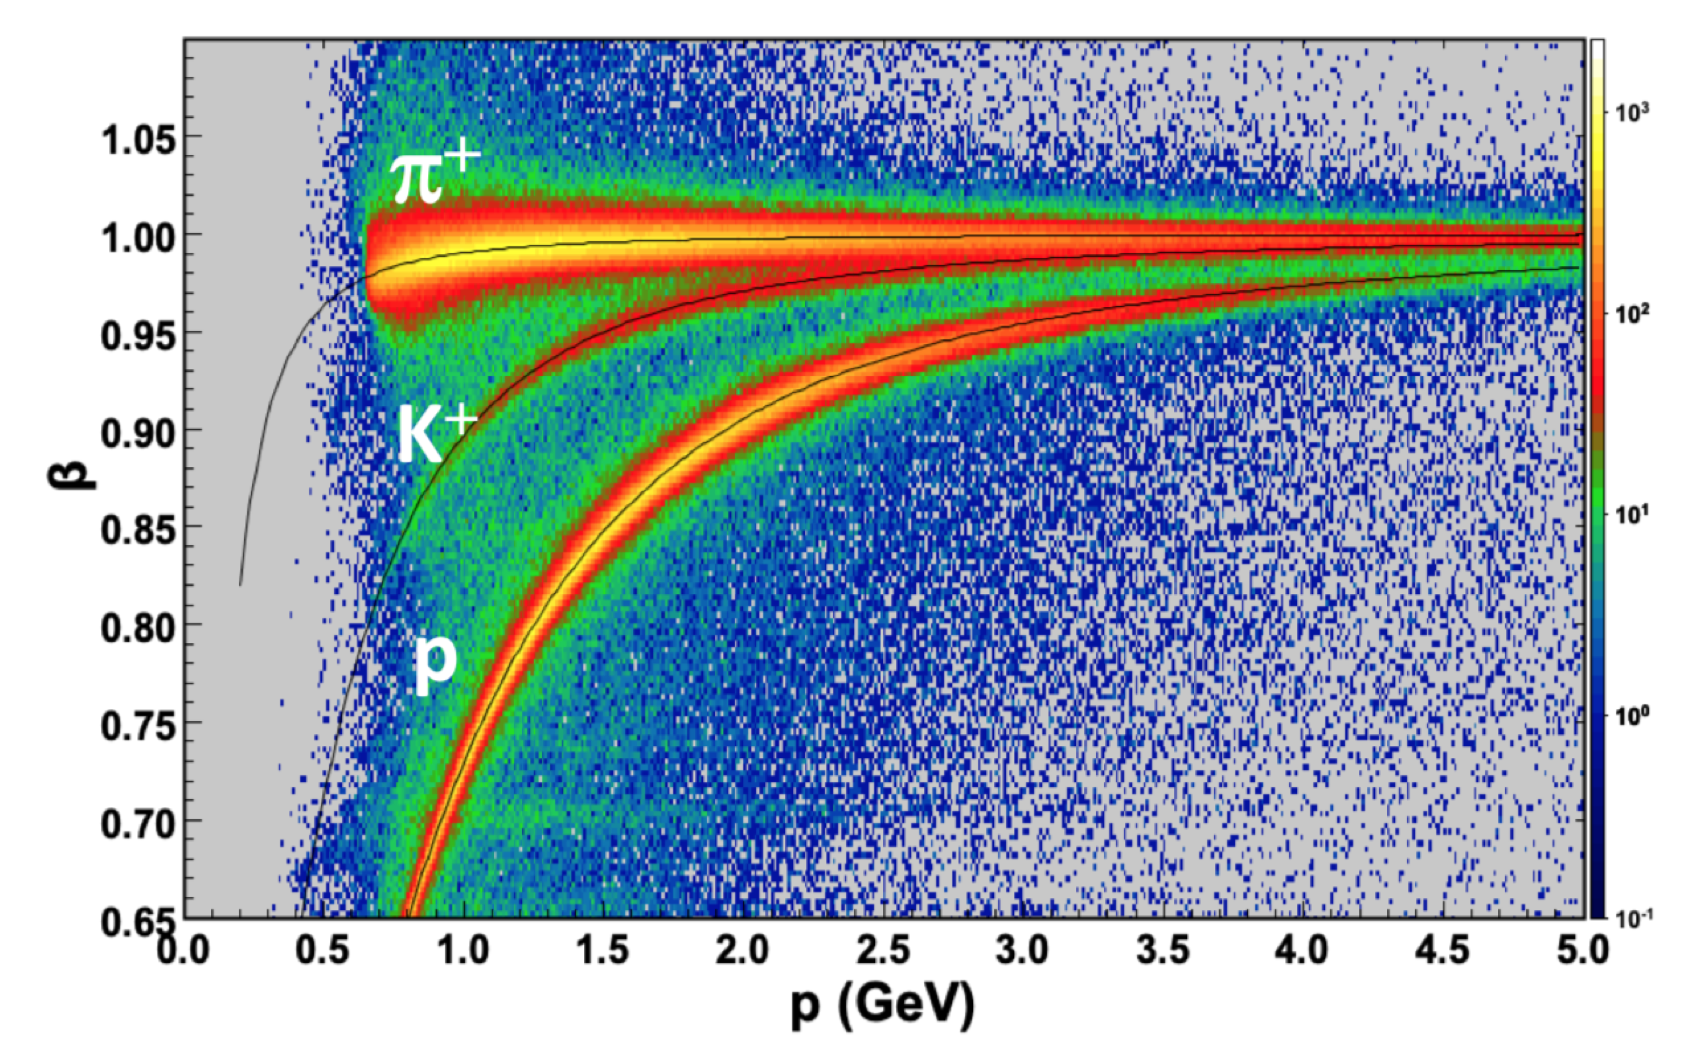
\includegraphics[width=0.25\textwidth,natwidth=610,natheight=642]{FTOF1b_pid.png}}}
\end{picture} 
\caption{Velocity $\beta = v/c $ versus momentum of charged particles detected in the CLAS12 FD. The thin black lines show
  the expected distributions for the respective charged tracks. The particle ID is limited to momenta greater than 0.8~GeV
  when the Torus magnet is energized to maximum current. At reduced current the tracking is extended to lower momenta at
  the expense of momentum resolution. }
\label{pid}
\end{figure} 

Identification of charged particles in CLAS12 is achieved in a number of ways. Identified electrons are used to determine
the start time of hadrons at the production vertex. The start time and the path length of charged tracks from the production
vertex to the FTOF and the arrival time enable determination of the $\beta = v/c$ of the particle, shown in Fig.~\ref{pid}
versus particle momentum for positive charged tracks, and the mass projections are shown in Fig.~\ref{pid-1D}.  An overview
of the particle identification in the various CLAS12 detector systems vs. momentum is given in Fig.~\ref{pid1}. 

\begin{figure}[htbp]
\vspace{6.0cm}
\begin{picture}(50,50)
\put(0,-10)
{\hbox{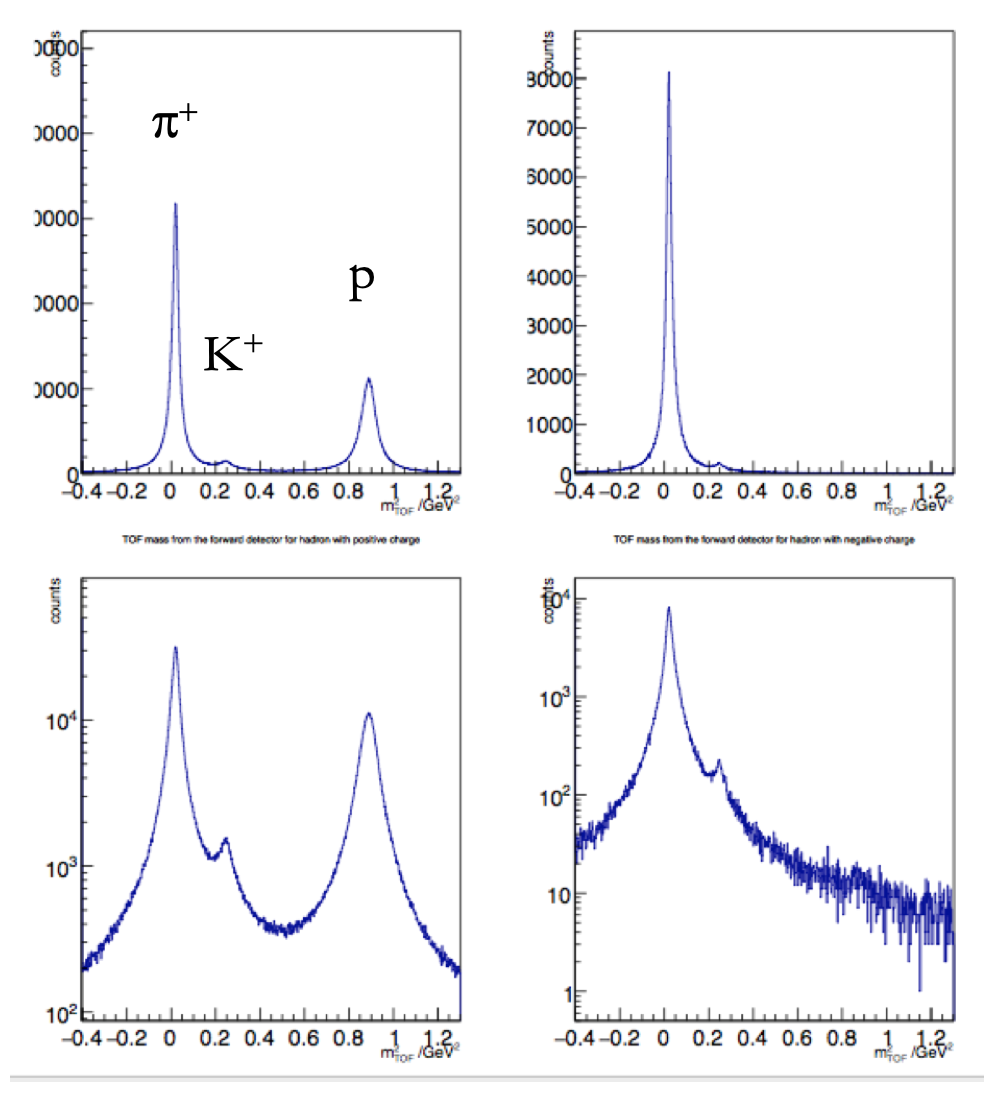
\includegraphics[width=0.40\textwidth,natwidth=610,natheight=642]{pid-1d.png}}}
\end{picture} 
\caption{Mass$^2$ of charged particles evaluated from their momentum and the time-of-flight information in the FTOF.
  Left: Positively charged hadrons: $\pi^+$, $K^+$, $p$. Right: Negatively charged hadrons: $\pi^-$, $K^-$, ${\bar{p}}$.
  {\bf Clean up graphs for publication.}}
\label{pid-1D}
\end{figure} 

\begin{figure}[htbp]
\vspace{4.0cm}
\begin{picture}(50,50)
\put(5,0)
{\hbox{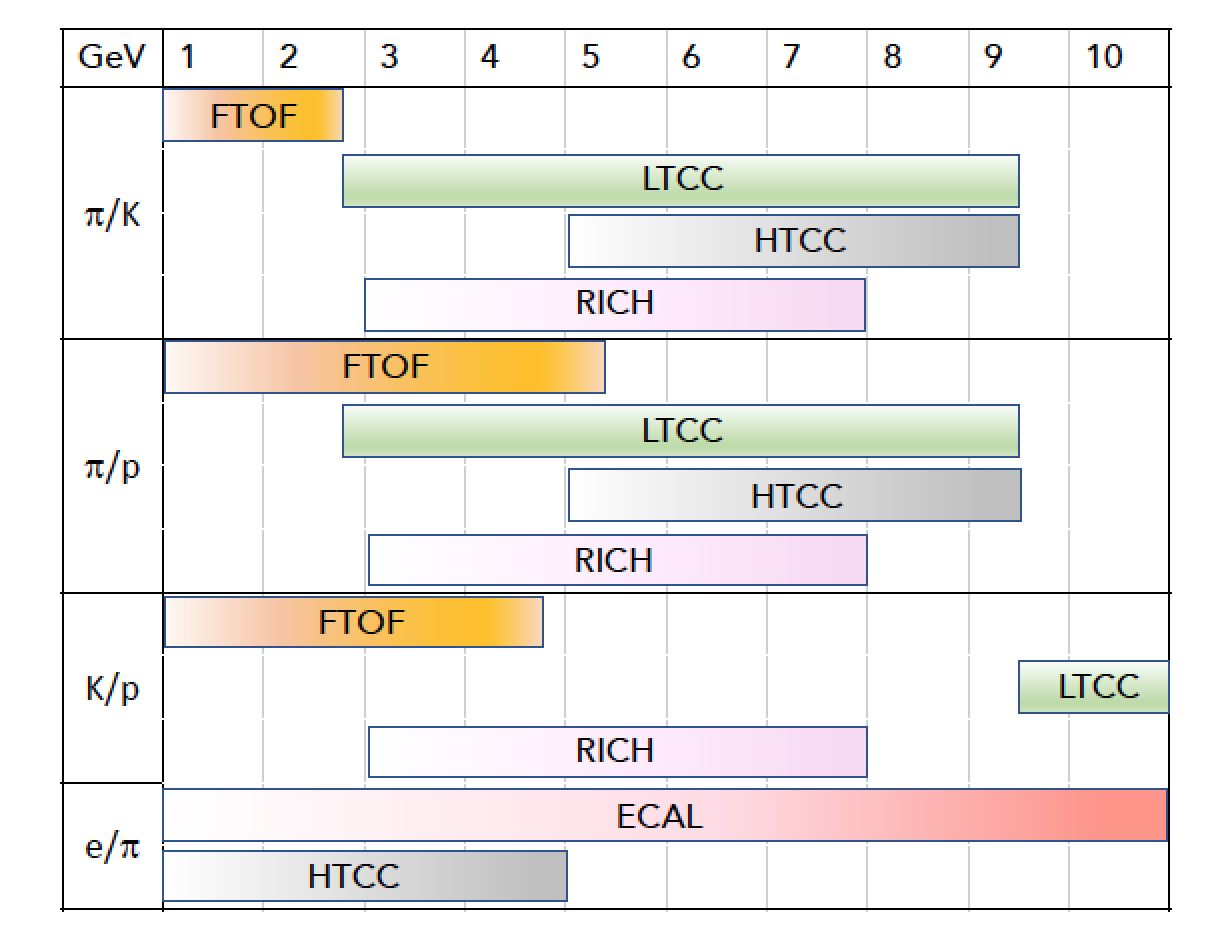
\includegraphics[width=0.32\textwidth,natwidth=610,natheight=642]{CLAS12-pid.png}}}
\end{picture} 
\caption{Overview of particle identification in various detectors of the CLAS12 FD. The higher (lower) intensity of the color
  shading indicates higher (lower) effectiveness for the particle species separation shown.  } 
\label{pid1}
\end{figure} 

The Fig.~\ref{spectrum} shows the inclusive spectrum $ep \to e^\prime X$ and the $ep \to e^\prime \pi^+ X$ with missing
neutron at four different beam energies. Fig.~\ref{elastic-peak} shows fits to the a elastic peak and to the missing neutron
mass distributions in 3 sectors at a beam energy of 10.6~GeV, and Fig.~\ref{pip-pim-p} shows for the reaction
$ep \to e' \pi^+ \pi^- X$ the invariant mass of $\pi^+\pi^-$ and the missing mass $M_X$.  

\begin{figure*}[htbp]
\vspace{5.0cm}
\begin{picture}(50,50)
\put(75,0)
{\hbox{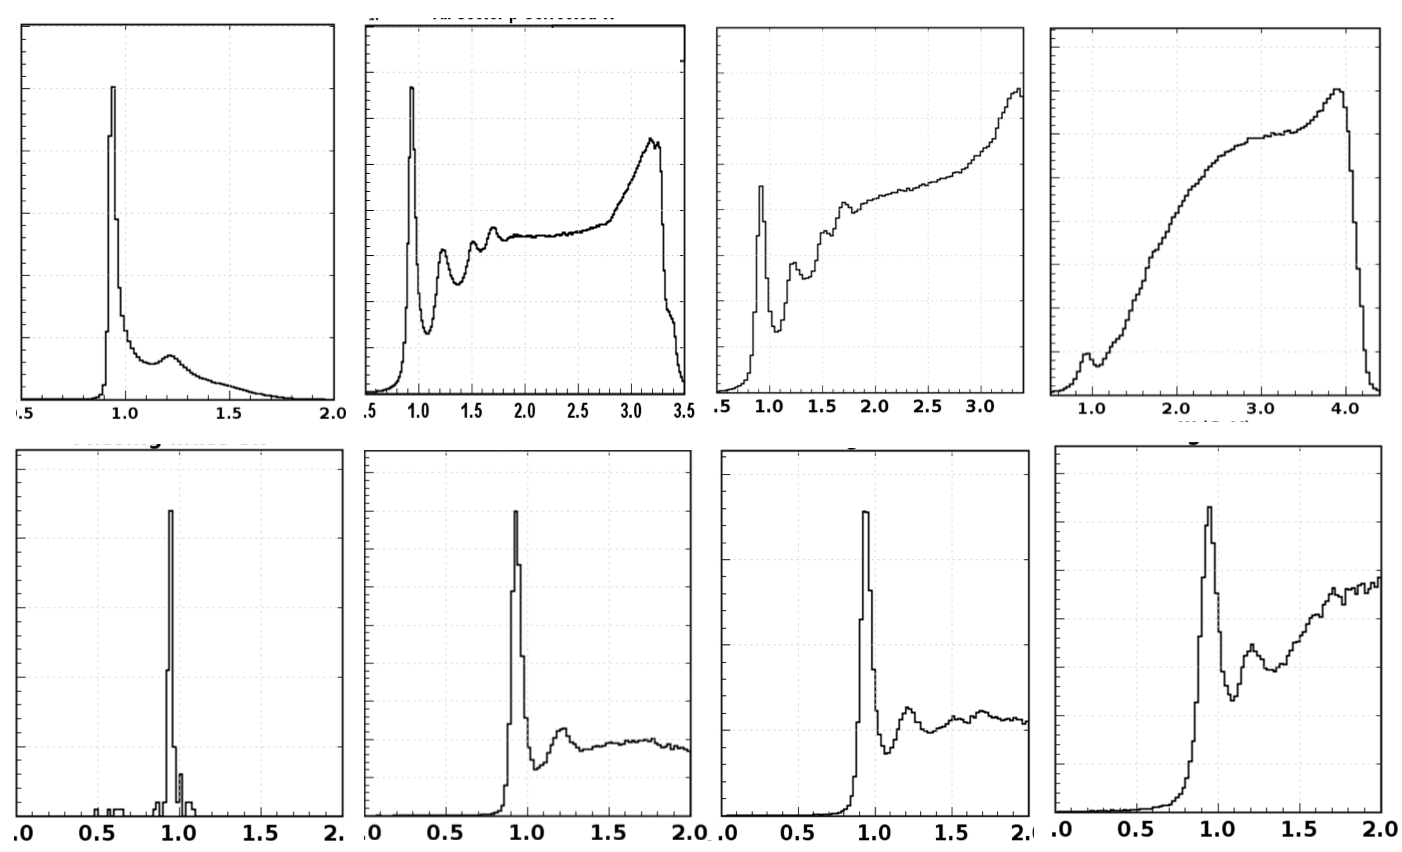
\includegraphics[width=0.40\textwidth,natwidth=610,natheight=642]{W-spectrum.png}}}
\end{picture} 
\caption{Upper row: Inclusive electron scattering spectrum $ep \to e^\prime X$ measured in CLAS12 at beam energies 
  of 2.2~GeV, 6.5~GeV, 7.5~GeV, and at 10.6~GeV (from left to right). The peak to the left is due to elastic $ep \to ep$
  scattering. Enhancements from the first 3 excited nucleon states, $\Delta(1232)$, $N(1520)$, and $N(1680)$, are also
  visible for the lower beam energies. Note that the mass ranges  are different for the different beam energies. Lower row:
  Missing mass distributions of $ep\to e' \pi^+X$ for the same energies. The sharp mass peak to the left is due to  the
  undetected neutron. The second peak for the higher energies is due to the $\Delta^0(1232)$. The horizontal axes are in
  units of~GeV. {\bf Need some arbitrary vertical scale and energy IDs in the figures.}} 
\label{spectrum}
\end{figure*} 

\begin{figure}[htbp]
\vspace{6.0cm}
\begin{picture}(50,50)
\put(8,0)
{\hbox{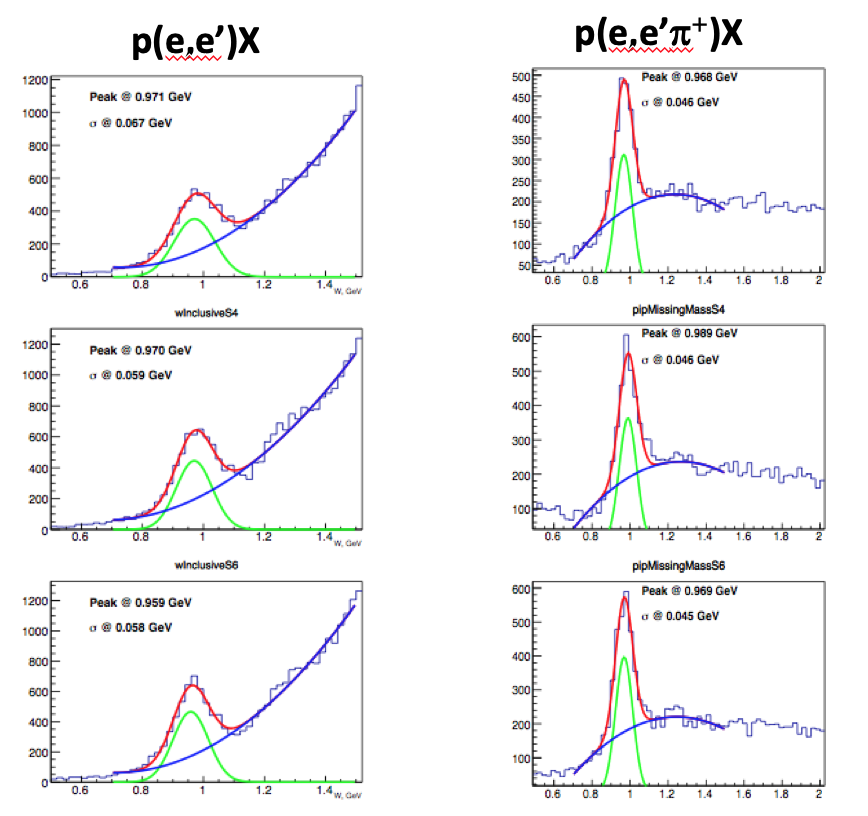
\includegraphics[width=0.45\textwidth,natwidth=610,natheight=642]{elastic_pi+n.png}}}
\end{picture} 
\caption{ The left panels show the elastic peak at 10.6~GeV beam energy as measured in 3 sectors. The peak is close to the
  proton mass in all sectors reflecting the good momentum calibration of all sectors. A fit to the elastic signal shows sector to
  sector variation of less than {\bf XX MeV} ({\bf need to replace after kinematic corrections have been applied}). The
  right panels show the mass distribution of the unmeasured final state X in $ep \to e\pi^+ X$. The peak is due to the unmeasured
  neutron.{\bf replace after kinematic corrections are applied.} The mass resolution $\sigma_X$ is 45~MeV} 
\label{elastic-peak}
\end{figure} 

\begin{figure}[htbp]
\vspace{3.5cm}
\begin{picture}(50,50)
\put(8,-5)
{\hbox{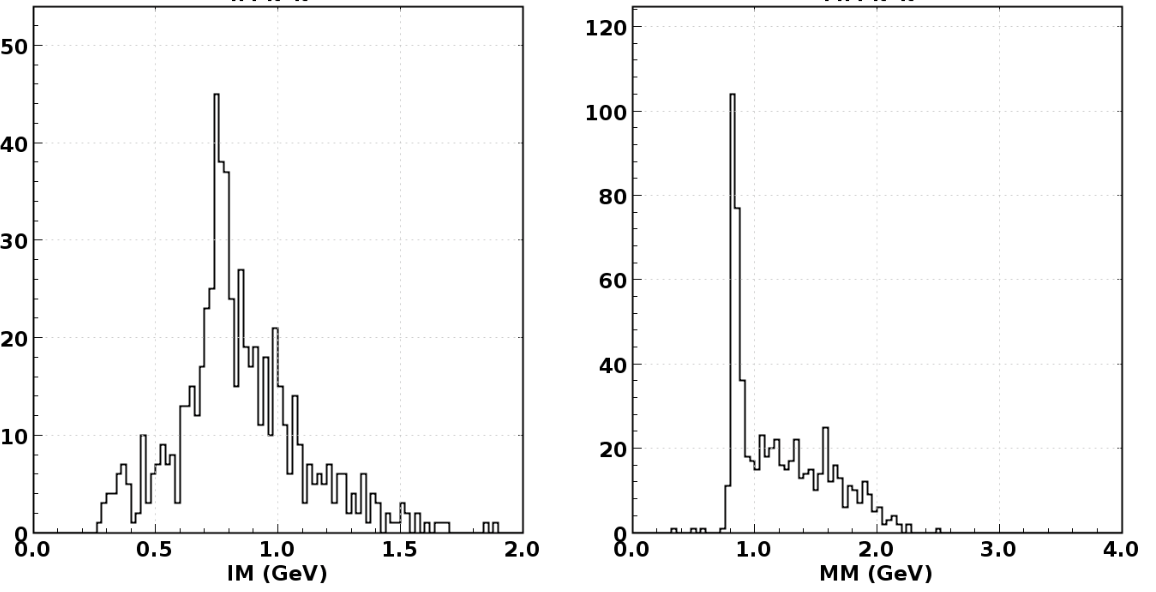
\includegraphics[width=0.33\textwidth,natwidth=610,natheight=642]{pip-pim-p.png}}}
\end{picture} 
\caption{Left: Invariant mass of $\pi^+\pi^-$, showing the peak at the $\rho^\circ$ mass. Right: missing mass
  $M_X$  of $e^-\pi^+\pi^-X$ with the peak at the proton mass that establishes the exclusive process
  $ep\to e' p \pi^+\pi^-$. ({\bf waiting for better statistics after cooking.)}}
\label{pip-pim-p}
\end{figure} 

\subsection{Charged Particle Detection in CD}

{\bf Include a section on tracking and particle identification in the CD} Momentum reconstruction in the CVT combined
with the timing information from the CTOF allows for the separation of charged pions from charged kaons and protons in the
momentum range from 0.25~GeV to 1.5~GeV. The momentum range covers a large part of the phase space allowed by the
maximum beam energy for hadron electroproduction on hydrogen targets. Fig.~\ref{CD-PID} shows the particle velocity
$\beta = v/c$ versus the particle momentum reconstructed in the CVT.

\begin{figure}[htbp]
\vspace{4.0cm}
\begin{picture}(50,50)
\put(10,-10)
{\hbox{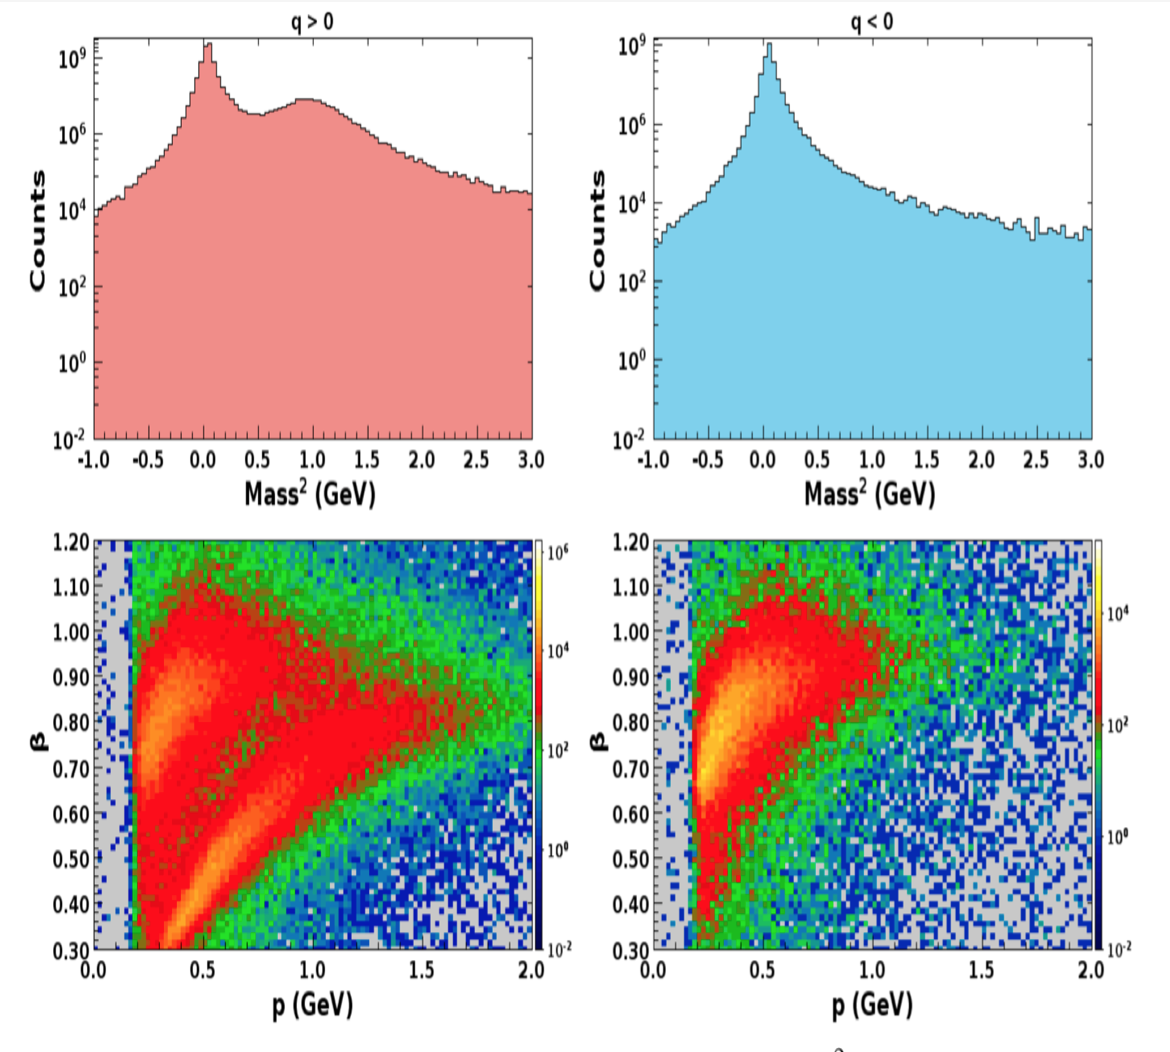
\includegraphics[width=0.32\textwidth,natwidth=610,natheight=642]{CTOF-PID.png}}}
\end{picture} 
\caption{Reconstructed mass$^2$ and beta versus momentum for positively charged particles (left) and for negatively
  charged particles (right) versus momentum for all CTOF counters from data taken at 10.6~GeV beam energy.}
\label{CD-PID}
\end{figure} 

\subsection{Neutral Particle Detection} 

Direct detection of neutral particles is accomplished in the FD using the PCAL and EC calorimeters. The combined 20
radiation length is sufficient to identify high energy photons and reconstruct masses of parent particles, such as
$\pi^0\to \gamma \gamma$  or $\eta \to \gamma \gamma$. At very forward angles the FT provides photon detection
with significantly improved position and energy resolution in the polar angle range from 2.5$^\circ$ to 4.5$^\circ$.
Fig.~\ref{gg} shows the invariant mass of the $\gamma\gamma$ system in the CLAS12 FD and in the FT, respectively. 

\begin{figure}[htbp]
\vspace{6.0cm}
\begin{picture}(50,50)
\put(10,115)
{\hbox{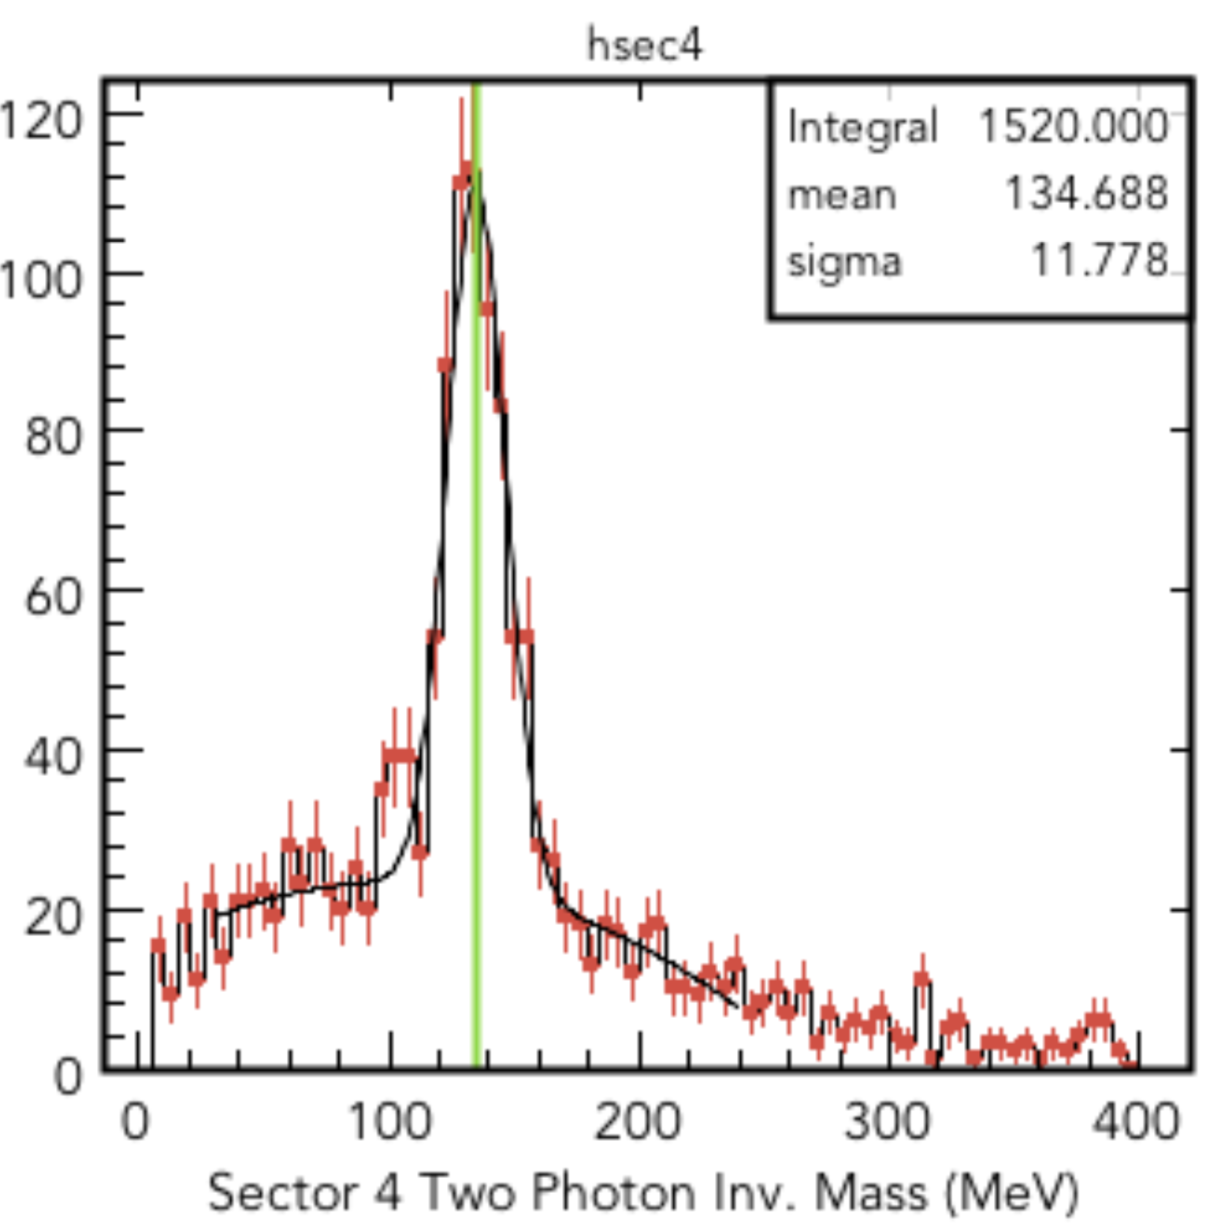
\includegraphics[width=0.30\textwidth,natwidth=610,natheight=642]{pi0.png}}}
\put(10,-5)
{\hbox{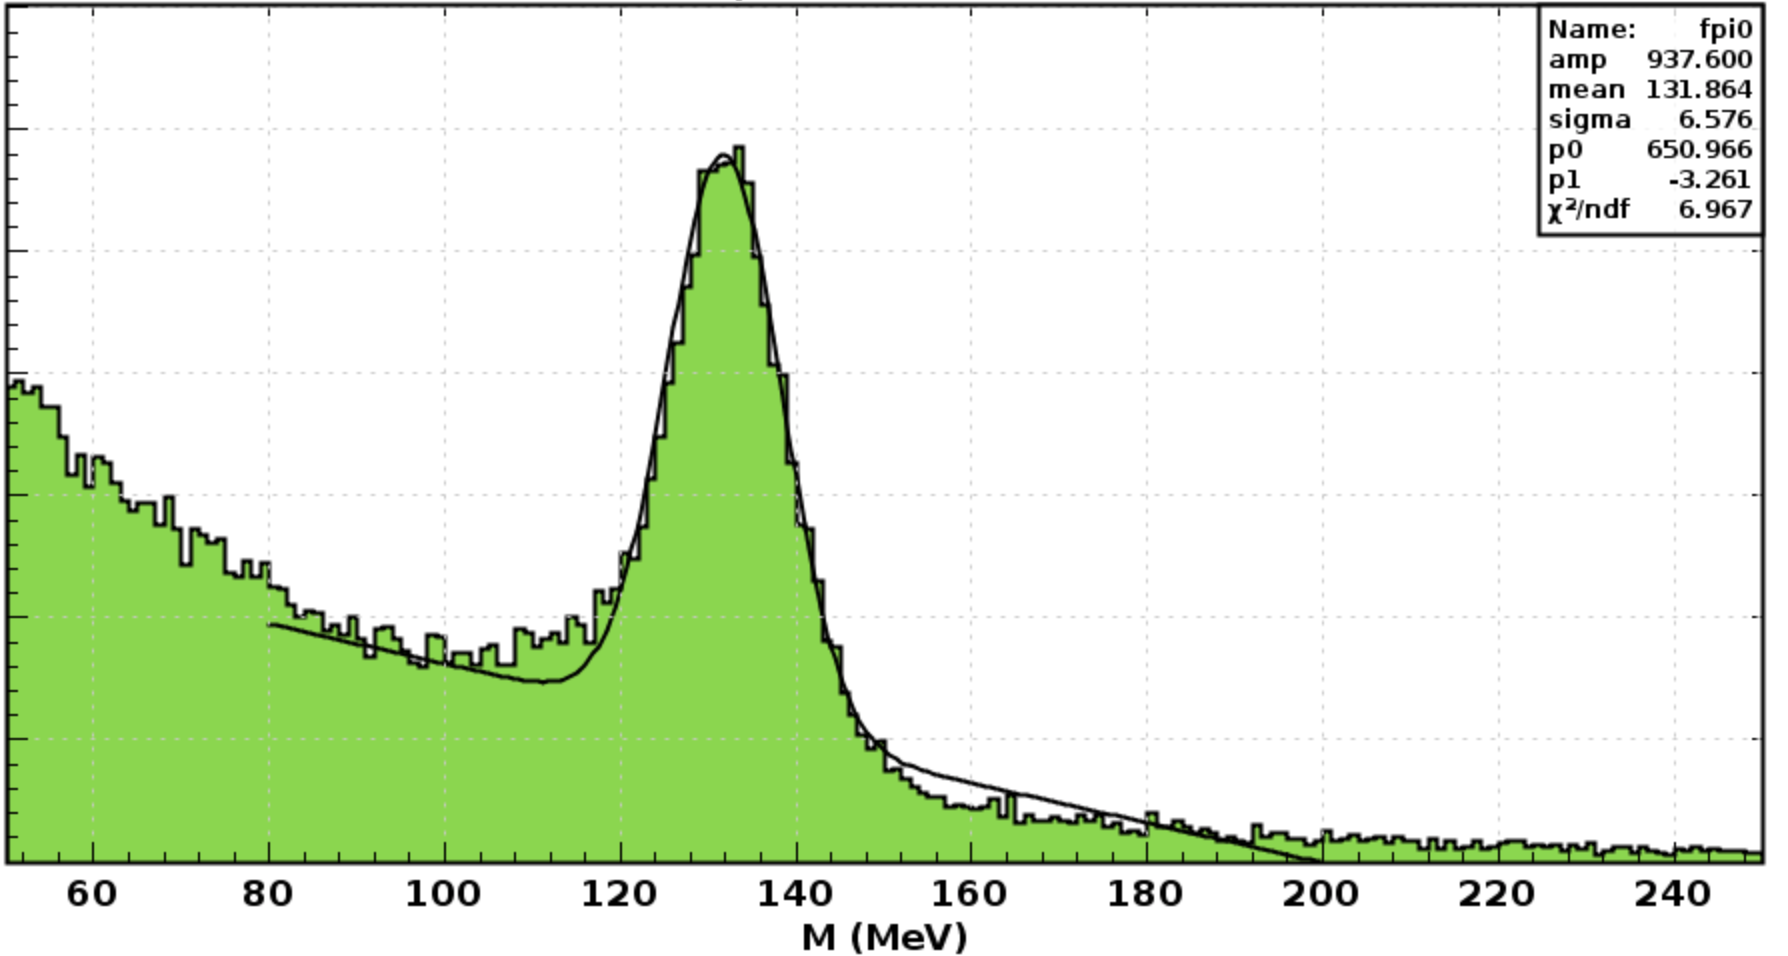
\includegraphics[width=0.21\textwidth,natwidth=610,natheight=642]{ft-pi0.png}}}
\end{picture} 
\caption{Top panel: The invariant mass of two high-energy photons in sector 4. The background underneath the $\pi^0$
  peak is due to multi-photon decays of higher mass mesons where one or more photons are not detected in the angle
  range covered by the calorimeter. The widths of the mass peak is 11.8~MeV. Bottom panel: The $\gamma\gamma$ mass
  for photons detected in the FT lead-tungstate crystal calorimeter, which has a significantly better mass resolution of the
  $\pi^0$ mass peak of 6.6~MeV. The FT covers the full azimuthal range of $360^\circ$, but only a $2.0^\circ$ range in polar
  angle range around the beamline. {\bf NEED BETTER GRAPHS.}} 
\label{gg}
\end{figure}

Neutral particle detection in the CD is provided by the CND combined with the CTOF. The polystyrene plastic scintillator
bars of the two detectors have a combined 15\% nuclear interaction length resulting approximately in a 12\% efficiency for
the detection of high energy neutrons. The plastic scintillators contribute about 29\% of a radiation length at $90^\circ$
polar angles; they are also detecting high energy photons through their conversion in $e^+e^-$ pairs. The discrimination of
photons and neutrons in the CD is  accomplished by the timing resolution of $75$~ps provided by the CTOF and the $150$~ps
of the CND. The separation of neutral particles from charged particle hits in the CND or in the CTOF is efficiently achieved
by using the CVT tracker to veto against false neutral hits in the CTOF and CND.  Fig.~\ref{CND-neutrals} shows the velocity
versus the energy deposition of charged and neutral particles in the CND.  

\begin{figure}[htbp]
\vspace{7.0cm}
\begin{picture}(50,50)
\put(22,125)
{\hbox{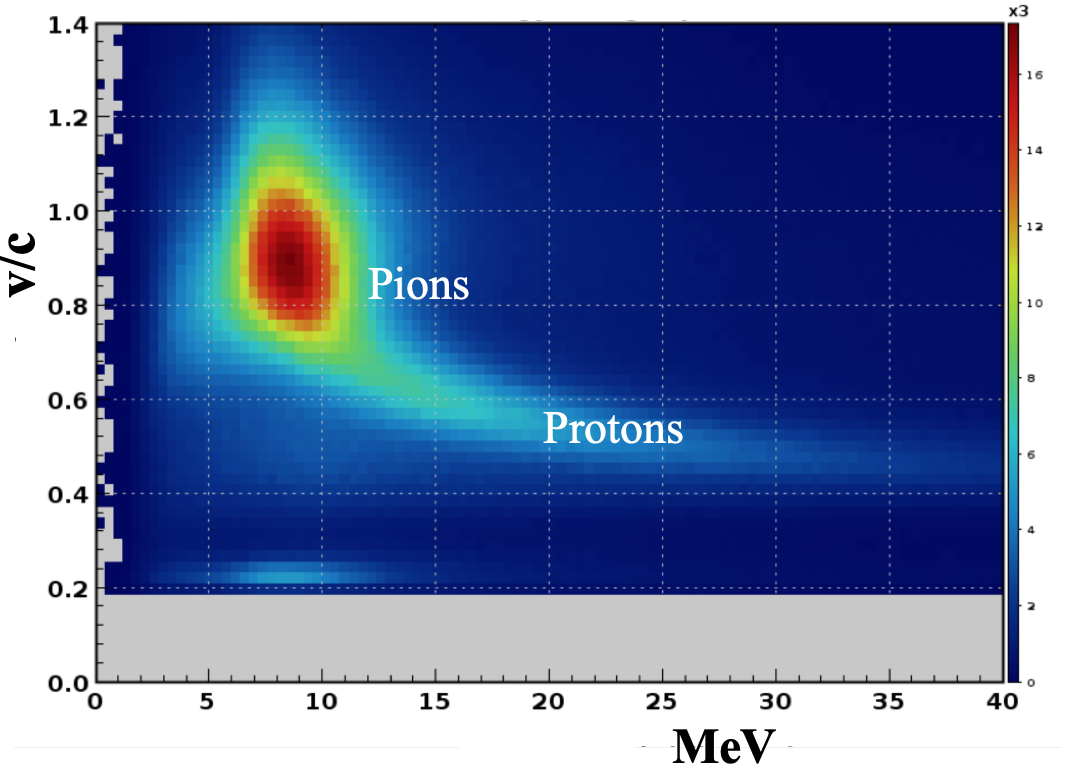
\includegraphics[width=0.30\textwidth,natwidth=610,natheight=642]{CND1.png}}}
\put(22,-5)
{\hbox{\includegraphics[width=0.30\textwidth,natwidth=610,natheight=642]{CND2.png}}}
\end{picture}
\caption{Top panel: Distribution of $v/c$ for charged particles in the CND, the deposited energy is correlated with a track
  in the CVT. Evidence for charged pions and protons is clearly visible.  Bottom panel: The same for neutral particles; no
  charged tracks are correlated to the energy deposited in the CND scintillators. The cut at v/c = 0.2 eliminates background
  events from accidental hits. {\bf NEED BETTER GRAPHS.}} 
\label{CND-neutrals}
\end{figure} 

\begin{figure}[htbp]
\vspace{6.0cm}
\begin{picture}(50,50)
\put(0,0)
 {\hbox{\includegraphics[width=0.27\textwidth,natwidth=610,natheight=642]{clas12-daq.png}}}
\end{picture}
\caption{Schematic diagram of the CLAS12 data acquisition and trigger system.}
\label{daq}
\end{figure}

\section{Data Acquisition and Trigger System} 

\subsection{CLAS12 Data Flow and Monitoring} 

During data taking the quality of the data is continuously monitored by displaying a very small fraction of single events
in the CLAS12 event display (ced) that allows immediate action by the shift personnel in case of obvious issues.
Monitoring histograms are filled on a regular basis that include simple analysis and can be easily compared with
histograms collected earlier during the data taking.  

The CLAS12 data acquisition (DAQ) is a dead-time free system designed for an average of 20~kHz level 1 (L1) 
trigger rate, pipelined and for continuous wave operation. The sector-based  L1 triggers support streaming, subsystem 
hit patterns and energy summing with low threshold suppression.  The scalable trigger distribution scheme uses up to
128 front-end L1 crates. CLAS12 uses different programmable features for each detector that participates in the L1
trigger. The schematic diagram is shown in Fig.~\ref{daq}. In 2018 the DAQ has been run at trigger rates of typically
15~kHz and data rates of 500~MB/s with a live time of $> 95\%$. At somewhat lower live time of ~90\%, trigger rates
of 20~kHz and data rates of up to 1~GB/s have been achieved. Details of the design, functionality, and performance of
the CLAS12 DAQ are provided in  Ref.~\cite{DAQ}. 

\subsection{Fast and Selective Triggers} 

CLAS12 uses a series of fast triggers that are tailored to a specific event pattern selection. Most of the physics
experiments require the electron scattered on the production target to be detected as it defines the mass ($Q^2$)
and kinematics of the virtual photon as $Q^2 = -(e - e^\prime)^2$, where $e$ an $e'$ are the 4-momentum vectors
of the beam electron and of the scattered electron, respectively. The electron kinematics also defines the Bjorken
scaling variable $x_B$  and the missing mass $W$ defined as $W^2 = M^2 + 2M\nu - Q^2$, with $\nu = E_e - E_{e'}$,
and $M$ the mass of the target particle. The scattered electron is uniquely identified with signals in the HTCC, clustered
energy deposition  in the PCAL and EC, and track-related energy deposition in the FTOF detectors. To enhance section of
specific reactions in the accumulated data, additional charged particles in either the FD or the CD are selected in the
trigger in addition to the scattered electron. The CLAS12 fast trigger system makes use of the responses of the detectors
to events. At the design luminosities of CLAS12, the hadronic production rate is approximately $5 \times 10^6$/s. However,
only a small fraction of those events is of interest for the science program with CLAS12. In particular, most physics reaction
require the detection of the scattered electrons at some finite scattering angle, for example $\theta_{e'} > 5^\circ$.  
   
\begin{figure}[htbp]
\vspace{5.7cm}
\begin{picture}(50,50)
\put(0,-3)
{\hbox{\includegraphics[width=0.16\textwidth,natwidth=610,natheight=642]{trigger.png}}}
\end{picture} 
\caption{Predefined trajectories are employed to select hit patterns in the 3 drift chamber regions that correspond with
  hits in the FTOF and with localized energy deposition in the PCAL and EC. For the two-track trigger the two sectors show
  drift chamber hit patterns for tracks with opposite charges, the upper one bending towards the beamline, the lower one
  bending away from the beamline.}
\label{trigger}
\end{figure} 

In some special programs the detection of electrons in the FT is of interest if they are associated with hadronic event
patterns of additional 2 hadrons. Such conditions have been implemented in the fast trigger decision that reduces the
number of triggers to about $2 \times 10^4$ events /s, i.e. by  a factor of 250 from the hadronic rate. The data rate is
typically 500~MB/s under such conditions and can be handled by the CLAS12 data acquisition system and the available
computing resources. Fig.~\ref{trigger} shows one example of a hadron pair trigger. It uses the drift chamber roads,
associated signals in the FTOF, and energy deposition in the PCAL and EC that are consistent with two minimum ionizing
particles. This trigger has a near 100\% efficiency, and a 25\% purity. Another trigger is the inclusive electron trigger,
which in addition to the hadron trigger makes use of a correlated signals in the HTCC.  Details of the design, functionality,
and performance of the CLAS12 trigger are provided in  Ref.~\cite{DAQ}. 

\section{Electron Beam Operation} 

\subsection{Beamline}

The Hall~B beamline has two sections, the 2C line, from the beam switch yard (BSY) to the Hall proper, and the 2H line,
from the upstream end of the experimental Hall to the beam dump (or Faraday cup) in the downstream tunnel, as shown in 
Figs.~\ref{beamline-upstream} and \ref{beamline-downstream}. The beamline instrumentation consists of beam-optics,
beam position and beam current monitors, beam viewers, collimators,  shielding, beam profile scanners, and beam halo
monitors. Devices that control the beam direction, its profile, and  measure critical parameters, are under the accelerator
operations control. Hall~B operators control collimators, halo monitors, profile scanners, and viewers. 

The magnet on the left (in red) is not energized during production data taking. It is used during beam tuning before the beam
is directed on the Hall~B production target. It is also used during specialized runs, such as polarization measurements in the
upstream beamline, to avoid exposure of sensitive CLAS12 detectors to high background loads. For details of the beamline
elements and beam quality, see Ref.~\cite{beamline}.  
 
\begin{figure*}[ht]
\vspace{3.5cm}
\begin{picture}(50,50)
\put(10,-5)
{\hbox{\includegraphics[width=0.40\textwidth,natwidth=610,natheight=642]{beamline-upstream.png}}}
\end{picture} 
\caption{Hall B beamline upstream of the target, showing the photon tagger magnet to the left. The main element on the
  right is the solenoid magnet nearly fully encapsulated by the HTCC PMT housing. Several of the Torus magnet coils are
  visible at the far right.}
\label{beamline-upstream}
\vspace{1.4cm}
\begin{picture}(50,50)
\put(35,0)
{\hbox{\includegraphics[width=0.45\textwidth,natwidth=610,natheight=642]{beamline-downstream.png}}}
\end{picture} 
\caption{Beamline downstream of CLAS12 with the beam blocker and the Faraday cup at the downstream end.  {\bf Replace
  this graph with beamline upstream of the tagger magnet.}}
\label{beamline-downstream}
\end{figure*}

\subsection{Unpolarized Production Targets} 

Hall~B experiments are grouped into running periods according to beam energy and target material. The most often used
target materials have been liquid hydrogen and liquid deuterium. Other materials are solid nuclear targets of various kind
from $^4$He, $^{12}$C, and $^{208}$Pb, dependent on the physics requirements. All targets are positioned inside CLAS12
using support structures that are inserted from the upstream end, and are independent of the detector itself.

\subsection{Polarized Production Targets} 

A large science program with CLAS12 requires the use of spin-polarized protons and neutrons. Spin-polarized protons and
polarized neutrons are used in compound material where the hydrogen or deuterium can be spin polarized using
microwave-induced electron spin transitions in molecules such as in NH$_3$ and ND$_3$. Certain electron spin-flips
can be transferred to the proton or neutron in the hydrogen or deuterium atoms, and lead to high polarization of up to 90\%
for the free protons, and over 50\% in neutrons of the deuterium atoms in this process of dynamical polarization. To achieve 
high levels of polarization, a high magnetic field of 5~T is required. In CLAS12, the required magnetic field is externally 
provided by the 5~T field in the center of the Solenoid magnet, which has been designed to provide a homogeneous magnetic
field of $\Delta B / B_0 \leq 10^{-3}$ within a cylindrical region of diameter $\phi = 2.5$~cm and $\Delta{z} = 4$~cm along
the beamline. The region near the target cell includes additional correction coils to achieve a factor 10 better homogeneity,
that is needed for polarizing the deuterium nuclei in ND$_3$. Other polarized material, such as polarized HD (called HD-Ice)  
will also be used in support of programs that require spin-polarized targets with the polarization axis oriented transverse to
the direction of the electron beam.        

\begin{figure}[htbp]
\vspace{4.2cm}
\begin{picture}(50,50)
\put (0,-10)
{\hbox{\includegraphics[width=0.45\textwidth,natwidth=610,natheight=642]{DC1-occupancy.png}}}
\end{picture} 
\caption{Accidental occupancies in the DC R1 versus the beam current, with the Solenoid magnet at full field. The
  measurement was carried out with the FT in the OFF configuration (red line). The dependence on the beam current
  is linear. At 75~nA beam current the measurement was also done in the FT in the ON configuration (green), and the
  occupancy increased by 50\%.}
\label{occupancies1}
\end{figure}

\begin{figure}[htbp]
\vspace{4.5cm}
\begin{picture}(50,50)
\put (0,-5)
{\hbox{\includegraphics[width=0.34\textwidth,natwidth=610,natheight=642]{occupancy-solenoid.png}}}
\end{picture} 
\caption{Accidental occupancies in the 3 regions of DC versus the current in the solenoid magnet. The measurement
  was carried out with the FT in the ON configuration. The sensitivity on the solenoid current comes from the fact that
  the primary source is charged particles, especially M{\"o}ller  electrons. The sensitivity is strongest for DC R1.}
\label{occupancies2}
\end{figure}

\subsection{Luminosity Constraints on CLAS12 Operations}

CLAS12 is designed for a significantly higher luminosity compared to CLAS. However, the high luminosity operation 
has measurable effects on the hit occupancy in the drift chambers and on the resolution in the momentum reconstruction.
Also, the reconstruction efficiency of charged particles can be affected. Fig.~\ref{occupancies1} and \ref{occupancies2}
show the hit occupancies in the drift chambers for different beam currents and for different current in the Solenoid magnet,
respectively. These effects can be studied in simulations when the beam conditions can be realistically imposed on the data.
For that purpose a procedure was developed that takes randomly triggered events at the operating beam current and
superimposes these events on the simulated events without the background. In this way one can study the reconstruction
efficiencies as a function of luminosity of the actual experiment. With increasing luminosity accidental, out-of-time events can
affect and alter particle tracks that come in-time. The most important effect is that the track quality is negatively affected
leading to track losses if stringent quality requirements are applied. This is demonstrated in Table~\ref{resolution}.    

\begin{table}[htbp!]
\caption{Impact of high current operation on resolutions in single track reconstruction.}     
\vspace{0.2cm}\label{resolution}
\small
\begin{tabular}{|c|c|c|c|c|}
\hline
&&&&\\
Parameter & Current &Shift & Resolution &Specs\\
&&&&\\
\hline
& 0~nA & - 0.083 & 0.52 & \\
$\Delta{p}/p$~(\%) &60~nA & -0.083 & 0.67& $\le 1$\\
& 120~nA & -0.08 & 0.86 &  \\
\hline 
&0~nA & -0.35 & 3.3 &  \\
$\Delta \phi$~(mrad) & 60~nA & -0.31& 3.8 &  $\le 4.5$\\
&120~nA & -0.47 & 4.4 &  \\
\hline
&0~nA & -0.055 & 0.66 &  \\
$\Delta \theta$~(mrad)& 60~nA & -0.070 & 0.85 &  $\le 1$\\
&120~nA & -0.035 & 0.85 &  \\
\hline
& 0~nA & -0.14 & 3.5 &  \\
$\Delta{V_z}$~(mm) & 60~nA & -0.23 & 4.6 & -  \\
& 120~nA & 0.04 & 5.6 & \\
\hline
\end{tabular}
\end{table}

\begin{figure}[htbp]
\vspace{6.0cm}
\begin{picture}(50,50)
\put (10,-5)
{\hbox{\includegraphics[width=0.25\textwidth,natwidth=610,natheight=642]{efficiencies.png}}}
\end{picture} 
\caption{(Color online) Impact of high luminosity operation on single track reconstruction.The curves show the tracking
  efficiency when certain quality constraints are imposed. About 6-7\% of the tracks are lost at 75~nA beam current
  corresponding to a luminosity of $10^{35}$~cm$^{-2}$s$^{-1}$ with no quality cuts. black: hit-based tracking, red: time-based
  tracking). The other curves show increasing tracking efficiency losses when increasingly more stringent quality cuts are
  applied on the missing mass  width. The process used is elastic muon-proton scattering where the proton mass is inferred
  from the elastic muon track, and compared with the known proton mass. At higher beam currents increasingly wider tails
  develop on the inferred proton mass. For the first run period in the spring and fall of 2018, the luminosity was limited to not
  exceed occupancies of 4\% in the R1 drift chambers. This typically resulted in about 45~nA to 60~nA of beam current, or
  about 60\% to 80\% of the design luminosity. }
\label{efficiencies}
\end{figure}
%\vfill\eject

\begin{figure}[htbp]
\vspace{3.8cm}
\begin{picture}(50,50)
\put (0,-10)
{\hbox{\includegraphics[width=0.40\textwidth,natwidth=610,natheight=642]{rich-event.png}}}
\end{picture} 
\caption{Top: Photo and detector response of the RICH MA-PMT array during beam operation. Bottom: One event with
  the ring of Cherenkov photons (left), and overlaid with expected rings from pion, kaon and proton at same momentum. The
  radius of the Cherenkov ring is consistent with a pion.}
\label{rich-event}
\end{figure}

Another way of quantifying the effect is by studying the number of lost tracks when certain quality requirements are
imposed. This is shown in Fig.~\ref{efficiencies}.  

\subsection{Performance of RICH} 

Figure~\ref{rich-event} shows the multi-anode photomultiplier array and a single Cherenkov event for a track with
the Cherenkov light detected in the MA-PMT array.  The performance in event reconstruction is illustrated in
Fig.~\ref{rich_rec} for negatively and positively charged particles. 

\begin{figure}[htbp]
\vspace{4.0cm}
\begin{picture}(50,50)
\put(0,-5)
{\hbox{\includegraphics[width=0.26\textwidth,natwidth=610,natheight=642]{RICH_rec.png}}}
\end{picture} 
\caption{Charged particle identification in the RICH detector. Note that pion/kaon separation sets in where it ranges out
  with the time-of-flight resolution in FTOF shown in Fig.~\ref{pid}.}
\label{rich_rec}
\end{figure}

\begin{figure*}[htbp]
\vspace{2.9cm}
\begin{picture}(50,50)
\put(0,-10)
{\hbox{\includegraphics[width=0.43\textwidth,natwidth=610,natheight=642]{charges.png}}}
\end{picture} 
\caption{Run periods in 2018 through spring 2019. The four periods are 1) commissioning, 2) spring 2018 data taking,
  3) summer/fall 2018 data taking, and 4) spring 2019 data taking.}
\label{charges}
\end{figure*}

\begin{figure}[htbp]
\vspace{6.7cm}
\begin{picture}(50,50)
\put(0,150)
{\hbox{\includegraphics[width=0.19\textwidth,natwidth=610,natheight=642]{cvt-cosmic-w-solenoid.png}}}
\put(0,0)
{\hbox{\includegraphics[width=0.22\textwidth,natwidth=610,natheight=642]{cvt-3-tracks.png}}}
\end{picture} 
\caption{Top: Example of cosmic ray tracks in the CVT with magnetic field B = 5~T. Left panel: Track projected to the
  plane perpendicular to the beamline. Right panel: The same track projected onto a plane along the beamline. Bottom:
  Multiple track event reconstructed in the CLAS12 Central Detector. Clockwise turning tracks in the solenoid magnetic
  field are from positively charged particles.}
\label{cvt-tracks}
\end{figure}

\begin{figure}[htbp]
\vspace{4.0cm}
\begin{picture}(50,50)
\put(0,-5)
{\hbox{\includegraphics[width=0.18\textwidth,natwidth=610,natheight=642]{cnd-performance.png}}}
\end{picture} 
\caption{Performance of the CND. Upper panels show the photomultiplier timing resolution and correlation in position
  projected from the CVT and the measurement of the CND. Bottom panels show particle $\beta$ versus momentum of
  the CND showing the $\pi^-$ band (left) and the proton and $\pi^+$ bands. {\bf Need to add plots for neutrals as
  well. See under neutrals in CD.}}
\label{cnd-performance}
\end{figure}

\begin{figure*}[htbp]
\vspace{3.2cm}
\begin{picture}(50,50)
\put(3,-5)
{\hbox{\includegraphics[width=0.30\textwidth,natwidth=610,natheight=642]{HTCC_1.png}}}
\put(158,-5)
{\hbox{\includegraphics[width=0.30\textwidth,natwidth=610,natheight=642]{HTCC_2.png}}}
\put(313,-5)
{\hbox{\includegraphics[width=0.30\textwidth,natwidth=610,natheight=642]{HTCC_3.png}}}
\end{picture} 
\caption{Acceptance distribution for scattered electrons in azimuthal angle for different bins in polar angle $\Theta$  - 
  left: $\theta = 5^\circ-7^\circ$, middle: $\theta = 13^\circ-15^\circ$, right: $\theta = 23^\circ-25^\circ$.  At these polar
  angle ranges the azimuthal acceptances are respectively 33\%,  66\%, and 80\% of the full sector range of $\pm 30^\circ$.
  Azimuthal angle coverage is symmetric around the sector mid-plane. The reduced acceptance at small polar angles is due to the
  cryostat of the Torus coils that are attached to a force ring at small angles limiting the geometrical acceptance to less than
  50\% in azimuthal angle. {\bf Needs higher statistics graphs} .}
\label{e-accept}
\end{figure*}

\begin{figure}[htbp]
\vspace{5.0cm}
\begin{picture}(50,50)
\put(2,-5)
{\hbox{\includegraphics[width=0.32\textwidth,natwidth=610,natheight=642]{cvt-acceptance.png}}}
\end{picture} 
\caption{CVT acceptance and tracking performance. Left panels show the tracking efficiency and acceptances for
  simulated muon tracks with no beam background (top), and the same for protons but with background corresponding
  to 50~nA beam current. The dips at 3 $\phi$ angles are due to support structure of the BMT tiles..}
\label{cvt-acceptance}
\end{figure}

\subsection{Tracks in the Central Detector}

Figure~\ref{cvt-tracks} shows selected track events in the CVT. The left panels show the projection to the plane
perpendicular to the beamline. In this view, positively charged particles bend clockwise in the 5~T magnetic field. The
innermost 3 double layers mark the SVT, the outer 6 layers indicate the BMT. The panels to the right show the projection
onto a plane along the beamline. The CTOF and CND detectors are located radially further away from the center and show
also deposited energy where the charged tracks hit. Uncorrelated hits are from out-of-time events. Other indicators of the
CND performance for charged particles are shown in Fig.~\ref{cnd-performance}.  

\subsection{Operating and Maintenance Experience}

The CLAS12 detector systems were commissioned in the period from December 2017 through February 2018, using beam
energies of 2.2, 6.4, and 10.6~GeV with both Torus magnet polarities, i.e. electrons bending towards the beamline, as well as
electrons bending away from the beamline, and data with different field strength settings in the Solenoid as well as in the
Torus magnet were carried. Understanding of the reconstructed events focused first on the lowest beam energy of 2.2.~GeV,
for which the elastic peak became quickly visible and could be used to understand the influence of the magnetic field map, 
overall detector geometry and the drift chamber alignments, among other parameters. After this initial commissioning period
data taking commenced for the Run Group A, which required use of a liquid hydrogen target. The allowed for the continuation of
the commissioning period while taken also production data. The ability to study exclusive processes played an essential role in
optimizing the operational performance. 

\subsection{Acceptances of the Forward Detectors} 

The science program with CLAS12 in general requires the detection of electrons that are scattered off the target material. 
For determining the kinematics of the reaction, the electrons must be identified and their 3-momentum determined by tracking
them in the magnetic field of the Torus magnet, and detecting them in the FTOF and in the EC, which covers approximately 
the polar angle range from $5^\circ$ to $35^\circ$. The detailed acceptance ranges depend also on the polarity of the 
magnetic field. Charged tracks that are deflected away from the beamline have acceptance functions that are different from
charged tracks that are deflected towards the beamline. The magnetic field of the Solenoid also affects the acceptance function
of charged particles. For opposite charges but same momentum the azimuthal rotation of scattered charged particles is same in
magnitude but opposite in sign.  Fig.~\ref{e-accept} shows the azimuthal acceptance at different polar angles for electrons
bending away from the beamline.  The electron acceptance of the HTCC is 360$^\circ$ in azimuth, but the acceptance for electron
tracks is reduced due to the cryostat of the Torus coils, which block electron transmission to the DC tracking system. The blockage
is largest at the smallest polar angle of $5^\circ$ and smallest at the largest polar angle of  $35^\circ$. This is shown 
in Fig.~ \ref{e-accept} at 3 polar angles.  

The acceptance is a complex function of the phase space covered by the processes of interest and must be simulated in 
full detail to precisely extract cross sections and other physics observables.  For this purpose a full simulation package was
developed, based on Geant4. 

\begin{table*}[ht!]
\begin{center}
\caption{ Comparison of the current performance of CLAS12 with the specifications originally set for the project. 
  {\bf Need to put the real numbers in from the data analysis} }    
\vspace{0.2cm}\label{clas12-performance}
%\hspace{-0.3cm}
\footnotesize
\begin{tabular}{|c|c|c|}
\hline
&&\\
Capability &  Quantity & Status\\
&&\\
\hline
Coverage & Tracks (FD) & $5^\circ \le \theta \le 35^\circ $ \\
& Tracks (CD)& $40^\circ \le \theta \le 125^\circ$  \\
& Momentum & $p > 0.2$~GeV \\
& Photon angle (FD)& $5^\circ \le \theta_\gamma \le 35^\circ$ \\  
& Photon angle (FT)& $2.5^\circ \le \theta_\gamma \le 4.5^\circ$ \\  
& Neutron det. (FD) & $5^\circ \le \theta \le 35^\circ $ \\
& Neutron det. (CD) &  $ 40^\circ \le \theta \le 125^\circ$ \\
\hline
Resolution & Momentum (FD)& $\sigma_p =  0.5 - 1.5 \%$  \\
& Momentum (CD) & $\sigma_p  < 5\%$  \\
 & Pol. angles (FD) & $\sigma_\theta = \rm  1- 2$~mrad  \\
 & Pol. angles (CD) & $\sigma_\theta =  \rm 10- 20$~mrad \\
& Azim. angles (FD) & $\sigma_\phi  \le 1~{\rm mrad}/\sin\phi $ \\
& Azim. angles (CD) & $\sigma_\phi \le \rm 20$ mrad \\
 & Timing (FD) & $\sigma_T =\rm  30 - 80$~ps  \\
& Timing (CD) & $\sigma_T = \rm 60 - 70$~ps \\
& Energy ($\sigma_E / E$)  (FD) & $0.1 / \sqrt{E~({\rm GeV})}$ \\
& Energy ($\sigma_E / E$)  (FT) & $0.03 / \sqrt{E({\rm GeV})}$\\
\hline
Particle ID& $\pi/\rm K ~(3\sigma)$ & $\rm p \le 3.0$~GeV  \\
& $\rm K/p ~ 3\sigma)$  & $\rm p \le 4.0$~GeV \\
& $\pi / \rm p~ (3\sigma)$  & $\rm p \le 5.0$~GeV \\
\hline
Precision & Luminosity &  $L = 10^{35}$~cm$^{-2}$s$^{-1}$ \\
\hline
DAQ/Trigger &  Data Rate &  10~kHz  200~MB/s \\
\hline 
Magnetic field & Solenoid& $B_0=5$~T, $B_{max}=6.5$~T\\
& Torus & 0.5-2.0~Tm\\
\hline 
\end{tabular}
\end{center}
\end{table*}

\subsection{Acceptance and Performance of the Central Detectors} 

The Central Detector system covers approximate regions in polar angles from $35^\circ$ to $125^\circ$ and the full
$360^\circ$ in azimuth.  Fig.~\ref{cvt-acceptance} shows the acceptance and reconstruction efficiency for charged tracks
from simulations with background incorporated according to beam current. {\bf Need to add more graphs on performance
of CD ??}. The limited space in the CD makes charged particle identification at high momentum challenging. Current performance
in terms of PID and tracking resolution has still some distance to go to be close to the expected performance parameters.   

\section{Summary} 

The design criteria, construction details, and operational performance characteristics of the large-acceptance CLAS12 dual 
magnet spectrometer have been described. The spectrometer is now used to study electron-induced reactions at the
energy-doubled CEBAF electron accelerator. The spectrometer has been commissioned in an initial period early 2018, and is
now routinely operated in support of a diverse scientific program in the exploration of the internal quark structure of nucleons
and nuclei. The major performance criteria, most critically, the operation at  instantaneous luminosities up to 
$10^{35}$~cm$^{-2}$s$^{-1}$, have been met. They are summarized in Table~\ref{clas12-performance}. Further improvements 
in operational performance are part of the experimental programs as more stringent requirements become part of the 
research program.  

\vspace{0.5cm}

\noindent{\bf Acknowledgments}

\vspace{0.3cm}

We would like to acknowledge the outstanding efforts of the staff of the Accelerator and the Nuclear Physics Division at JLab
that have contributed to the design, construction, installation, and operation of the CLAS12 detector.  This work was supported
in part ..........{\bf incomplete}.

\vspace{2.5cm}

\noindent{\bf References} 


\begin{thebibliography}{99}

\bibitem{Mcallister:1956ng} 
  R.~W.~Mcallister and R.~Hofstadter,
  %``Elastic Scattering of 188-{MeV} Electrons From the Proton and the $\alpha$ Particle,''
  Phys.\ Rev.\  {\bf 102}, 851 (1956).
  doi:10.1103/PhysRev.102.851

\bibitem{Breidenbach:1969kd} 
  M.~Breidenbach {\it et al.},
  %``Observed Behavior of Highly Inelastic electron-Proton Scattering,''
  Phys.\ Rev.\ Lett.\  {\bf 23}, 935 (1969).
  doi:10.1103/PhysRevLett.23.935
  
\bibitem{Kuhn:2008sy} 
  S.~E.~Kuhn, J.-P.~Chen and E.~Leader,
  %``Spin Structure of the Nucleon - Status and Recent Results,''
  Prog.\ Part.\ Nucl.\ Phys.\  {\bf 63}, 1 (2009)
  doi:10.1016/j.ppnp.2009.02.001.
 
 \bibitem{Burkert:2018nvj} 
  V.~D.~Burkert,
  %``Jefferson Lab at 12~GeV: The Science Program,''
  Ann.\ Rev.\ Nucl.\ Part.\ Sci.\  {\bf 68}, 405 (2018).
  doi:10.1146/annurev-nucl-101917-021129 
  
\bibitem{Mecking:2003zu}
  B.~A.~Mecking {\it et al.},
  %``The CEBAF Large Acceptance Spectrometer (CLAS),''
  Nucl.\ Instrum.\ Meth.\ A {\bf 503} (2003).
  doi:10.1016/S0168-9002(03)01001-5

\bibitem{Leemann:2001dg} 
  C.~W.~Leemann, D.~R.~Douglas and G.~A.~Krafft,
  %``The Continuous Electron Beam Accelerator Facility: CEBAF at the Jefferson Laboratory,''
  Ann.\ Rev.\ Nucl.\ Part.\ Sci.\  {\bf 51}, 413 (2001).
  doi:10.1146/annurev.nucl.51.101701.132327

\bibitem{Baturin:2012zz}
  V.~Baturin {\it et al.},
  %``Dynamic magnetic shield for the CLAS12 central TOF detector photomultiplier tubes,''
  Nucl.\ Instrum.\ Meth.\ A {\bf 664} (2012)11, doi:10.1016/j.nima.2011.10.003

\bibitem{Amarian:2001zs} 
  M.~Amarian {\it et al.},
  %``The CLAS forward electromagnetic calorimeter,''
  Nucl.\ Instrum.\ Meth.\ A {\bf 460}, 239 (2001).
  doi:10.1016/S0168-9002(00)00996-7

\bibitem{Adams:2001kk} 
  G.~Adams {\it et al.},
  %``The CLAS Cherenkov detector,''
  Nucl.\ Instrum.\ Meth.\ A {\bf 465}, 414 (2001).
  doi:10.1016/S0168-9002(00)01313-9
  
\bibitem{SVT} M.A. Antonioli et al., 'CLAS12 Silicon Vertex Tracker' 
\bibitem{BMT} XX. YYY, 'CLAS12 Barrel Micromegas Tracker' 
\bibitem{CTOF} D. S. Carman et al., 'The Central Time-ofFlight System for CLAS12' 
\bibitem{CND} J. Bettane et al., 'The CLAS12 Central Neutron Detector'
\bibitem{HTCC} Y. Sharabian et al.  ' CLAS12 High Threshold Cherenkov Counter (HTCC)' 
\bibitem{DC} M.D. Mestayer et al., 'The CLAS12 Drift Chamber System'
\bibitem{LTCC} D. Anderson et al.. ' The CLAS12 Low Threshold Cherenkov Counter (LTCC)' 
\bibitem{RICH} M. Contalbrigo et al., 'The CLAS12 RICH Detector'  
\bibitem{FTOF} D.S. Carman et al., 'The CLAS12 Forward Time of Flight system', link to NIM article.(2001) 239-265.
\bibitem{ECAL} G. Asryan et al., 'The CLAS12 Forward Electromagnetic Calorimeter', 
\bibitem{PCAL} G. Asryan et al.,  The CLAS12 Preshower Calorimeter,
\bibitem{FT} M. Battaglieri et al, 'The Forward Tagger for CLAS12' 
\bibitem{beamline} N. Baltzell et al., 'CLAS12 Beamline and ist Performance' 
\bibitem{DAQ} S. Boiarinov et al., 'CLAS12 Data Acquisition System' 
\bibitem{GEMC} D.S. Carman et al., 'CLAS12 Geant4 Simulations' 
\bibitem{Software} V. Ziegler et al., 'CLAS12 Event Reconstruction Software' 
\bibitem{clas12-magnets} R. Fair et al., 'Superconducting magnets for CLAS12'
\end{thebibliography}
\end{document}
 
 \begin{table*}[ht!]
\caption{ Comparison of the current performance of CLAS12 with the specifications originally set for the project. }     
\vspace{0.2cm}\label{clas12-performance}
\small
\begin{tabular}{|c|c|c|c|}
\hline
&&&\\
Capability &  Quantity &Specification& Achievement\\
&&&\\
\hline
Coverage&Charged particle FD & $5^\circ < \theta < 35^\circ $  & $5^\circ < \theta < 35^\circ $ \\
&Charged particle CD& $40^\circ < \theta < 125^\circ$ & $40^\circ < \theta < 125^\circ$  \\
&Momentum& $ p > 0.2~GeV$ & $p > 0.3~GeV$  \\
&Photon angle (FD)& $5^\circ < \theta_\gamma < 35^\circ$ & $5^\circ < \theta_\gamma < 35^\circ$\\  
&Photon angle (FT)& $2.5^\circ < \theta_\gamma < 4.5^\circ$ & $5^\circ < \theta_\gamma < 35^\circ$\\  
&Neutron detection (FD) & $5^\circ < \theta < 35^\circ $ & $ 5^\circ < \theta < 35^\circ$  \\
& Neutron detection (CD) &  $ 40^\circ < \theta < 125^\circ$ & $40^\circ < \theta < 125^\circ $\\
\hline
Resolution & Momentum (FD)& $\sigma_p =  0.5 - 1.5 \%$ & $\sigma_p < 1\%$  \\
& Momentum (CD) & $\sigma_p  < 5\%$ & $\sigma_p < 3\%$  \\
 & Polar angles (FD) & $\sigma_\theta = \rm  1- 2 mrad$ & $\sigma_\theta < \rm 2 mrad$  \\
 & Polar angles (CD) & $\sigma_\theta =  \rm 10- 20 mrad$ & $\sigma_\theta < \rm 20 mrad$  \\
& Azimuthal angles (FD) & $\sigma_\phi  < \rm 1 mrad/\sin\phi $ & $\sigma_\phi < \rm 3 mrad$  \\
& Azimuthal angles (CD) & $\sigma_\phi  < \rm 20 \rm mrad $ & $\sigma_\phi < \rm \rm 35 mrad$  \\
 & Timing (FD) & $\sigma_T =\rm  30 - 80~ps$  & $\sigma_T = 50 - 100~ps$  \\
& Timing (CD) & $\sigma_T = \rm 60 - 70~ps$  & $\rm \sigma_T < 100~ps$  \\
& Energy ($\sigma_E / E$)  (FD) & $\rm 0.1 / \sqrt{E(GeV)}$ & $\rm  0.1 / \sqrt{E(GeV)}$  \\
& Energy ($\sigma_E / E$)  (FT) & $\rm 0.03 / \sqrt{E(GeV)}$ & $ \rm 0.05 / \sqrt{E(GeV)}$  \\
\hline
Particle ID& $\pi/\rm K ~(3\sigma)$ & $\rm p \le3~GeV$ & $\rm p \le 2.5~GeV$  \\
& $\rm K/p ~ 3\sigma)$  & $\rm p \le 4.0~GeV$ & $\rm p \le 3.5~GeV $\\
& $\pi / \rm p~ (3\sigma)$  & $\rm p \le 5.0~GeV$ & $\rm p \le 4.5~GeV$\\
\hline
Luminosity &  &  $\rm L = 10^{35} \rm cm^{-2} s^{-1} $ & $\rm L = 10^{35} \rm cm^{-2} s^{-1} $ \\
\hline
Data acquisition &  Data Rate &  10~kHz,  200~MB/s  &  20~kHz,  800~MB/s \\
\hline 
Magnetic field & Solenoid & $\rm B_0 = 5T, B_{max} = 6.5T$& $\rm B_0 = 5T, B_{max} = 6.5T$ \\
& Torus & 0.5 - 2.0 ~Tesla-meter& 0.5 - 2.0 ~Tesla-meter \\
\hline 

\end{tabular}

\end{table*}
 

%\endinput
%%
%% End of file `elsarticle-template-harv.tex'.
\end{document}
